% Autor: Leonhard Segger, Jannik Tim Zarnitz
% Datum: 2017-10-30
\documentclass[
% Papierformat
a4paper,
% Schriftgröße (beliebige Größen mit „fontsize=Xpt“)
12pt,
% Schreibt die Papiergröße korrekt ins Ausgabedokument
pagesize,
% Sprache für z.B. Babel
ngerman
]{scrartcl}

% Achtung: Die Reihenfolge der Pakete kann (leider) wichtig sein!
% Insbesondere sollten (so wie hier) babel, fontenc und inputenc (in dieser
% Reihenfolge) als Erstes und hyperref und cleveref (Reihenfolge auch hier
% beachten) als Letztes geladen werden!

\usepackage{tikz}
\usetikzlibrary{calc,patterns,angles,quotes} % loads some tikz extensions\usepackage{tikz}
\usetikzlibrary{babel}

% Silbentrennung etc.; Sprache wird durch Option bei \documentclass festgelegt
\usepackage{babel}
% Verwendung der Zeichentabelle T1 (Sonderzeichen etc.)
\usepackage[T1]{fontenc}
% Legt die Zeichenkodierung der Eingabedatei fest, z.B. UTF-8
\usepackage[utf8]{inputenc}
% Schriftart
\usepackage{lmodern}
% Zusätzliche Sonderzeichen
\usepackage{textcomp}

% Mathepaket (intlimits: Grenzen über/unter Integralzeichen)
\usepackage[intlimits]{amsmath}
% Ermöglicht die Nutzung von \SI{Zahl}{Einheit} u.a.
\usepackage{siunitx}
% Zum flexiblen Einbinden von Grafiken (\includegraphics)
\usepackage{graphicx}
% Abbildungen im Fließtext
\usepackage{wrapfig}
% Abbildungen nebeneinander (subfigure, subtable)
\usepackage{subcaption}
% Funktionen für Anführungszeichen
\usepackage{csquotes}
\MakeOuterQuote{"}
% Zitieren, Bibliografie
\usepackage{biblatex}


% Zur Darstellung von Webadressen
\usepackage{url}
%chemische Formeln
\usepackage[version=4]{mhchem}
% siunitx: Deutsche Ausgabe, Messfehler getrennt mit ± ausgeben
\usepackage{floatrow}
\floatsetup[table]{capposition=top}
\usepackage{float}
% Verlinkt Textstellen im PDF-Dokument
\usepackage[unicode]{hyperref}
% "Schlaue" Referenzen (nach hyperref laden!)
\usepackage{cleveref}
\sisetup{
	locale=DE,
	separate-uncertainty
}
\bibliography{EIRE2018_References}

\begin{document}
	
	\begin{titlepage}
		\centering
		{\scshape\LARGE Protokoll zu \par}
		\vspace{1cm}
		{\scshape\huge Einführung in rechnergestütztes Experimentieren \par}
		\vspace{3cm}
		
		{\large Jannik Tim Zarnitz (E-Mail: j\_zarn02@wwu.de) \par}
		{\large Leonhard Segger (E-Mail: l\_segg03@wwu.de) \par}
		\vfill
		
		in der Woche 03.09.2018 bis 06.09.2018\par
		betreut von\par
		{\large Dr. Jürgen Berkemeier}
		
		\vfill
		
		{\large \today\par}
	\end{titlepage}
	\tableofcontents
	\newpage

%TODO Deckblatt prüfen
%TODO am Ende: Begriffe vereinheitlichen und Größe von Grafiken anpassen

	\section{Aufbau einer Sinus- bzw. Bessel-Funktion} \label{sinusfkt}
	
	Zunächst soll unter Verwendung des graphischen Programmiersystems \glqq LabVIEW\grqq\ eine Sinus-Funktion realisiert werden. Mithilfe der von LabVIEW zur Verfügung gestellten numerischen Operationen, Konstanten und Schleifen lässt sich ein Programm schreiben, welches eine Sinusschwingung $u$ der Form
	
	\begin{equation} \label{u}
	u(A,f,t,\varphi) = A \cdot \sin(2\pi f t + \varphi) \ ,
	\end{equation}
	
	\noindent umsetzt. Wobei $A$ die Schwingungsamplitude, $f$ die Frequenz und $\varphi$ die Phasenverschiebung bilden. Außerdem ist jedes $t$ durch 
	
	\begin{equation} \label{t}
	t = \frac{i}{N}
	\end{equation}
	
	\noindent gegeben. $N$ ist dabei die Zahl der Stützstellen und zugleich die Anzahl der zu berechnenden Wertepaare. Der Index $i$ kann Werte im Bereich zwischen $0$ und $N$ annehmen. Der besagte Programmcode befindet sich im Blockdiagramm von LabVIEW und ist in \cref{sinusbesselprogrammcode} zu sehen. 
	
	\begin{figure}[H]
		\centering
		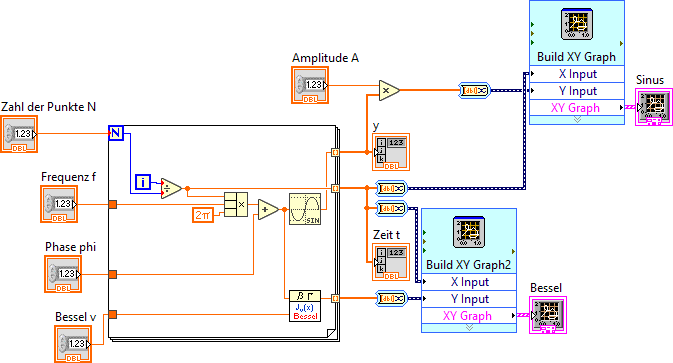
\includegraphics[width=1.0\textwidth]{EIRE2018Dateien/Tag1/sinusbessel-bilder/SinusBesseld}
		\caption{Die Abbildung zeigt ein LabVIEW-Blockdiagramm sowie den Aufbau des Programms zur Umsetzung einer Sinus- bzw. Bessel-Funktion. Die eigentliche Werte-Berechnung findet innerhalb der For-Schleife statt. Dazu werden feste, aber beliebige Fließkommazahlen für die Amplitude $A$, die Zahl der Punkte $N$, die Frequenz $f$, die Phase $\varphi$ und die Ordnung $\nu$ der Bessel-Funktion herangezogen. Die Ausgabe der Wertepaare erfolgt in Form zweier $X$-$Y$-Graphen sowie Arrays.}
		\label{sinusbesselprogrammcode}
	\end{figure}

	\noindent Das dazugehörige ausgegebene Frontpanel ist in \cref{sinusbesselausgabe} erkennbar. Die Gleitkommazahlen-Werte für $A$, $f$, $N$ und $\varphi$ sollen frei wählbar sein, zumal $u$ insbesondere von diesen abhängt. Das Programm ist daher so eingerichtet, dass auf der linken Seite des Frontpanels die entsprechenden Bedien- bzw. Eingabeelemente erscheinen. Unter gleichem Namen sind die jeweiligen Blockdiagrammobjekte im Programmcode zu finden. Im Zentrum des Programmcodes in \cref{sinusbesselprogrammcode} lässt sich eine For-Schleife erkennen. Gemäß \cref{u} sowie \cref{t} findet in dieser unter Verwendung des Laufindexes $i$ die tatsächliche Berechnung der $t$- und $u$-Werte statt. Die Blockdiagrammobjekte auf der rechten Seite des Programmcodes in \cref{sinusbesselprogrammcode} bilden die Anzeige- bzw. Ausgabeelemente des Frontpanels in \cref{sinusbesselausgabe}. Zum einen werden dabei zwei $N+1$ Einträge umfassende, eindimensionale Arrays angelegt, die jeweils alle $t$- sowie sämtliche $u$-Werte beinhalten und zum anderen wird ein $X$-$Y$-Diagramm erzeugt, in dem alle $u$-Werte gegen die entsprechenden $t$-Werte aufgetragen sind. Demnach befindet sich $t$ auf der $x$-Achse und $u$ auf der $y$-Achse. Um nun die Informationsübertragung zu bewerkstelligen, ist es notwendig im Programmcode vor den Anschlüssen der \glqq Build XY Graph\grqq -Kästen weitere Blockdiagrammobjekte hinzuzufügen, welche das Leitungssignal in ein für das Anzeigeelement ($X$-$Y$-Diagramm) passendes Eingangssignal umwandeln. Zumeist geschieht dies in LabVIEW automatisch und wird dann an der entsprechenden Stelle auf der Leitung mit einem kleinen, roten Punkt markiert.
			
	\begin{figure}[H]
		\centering
		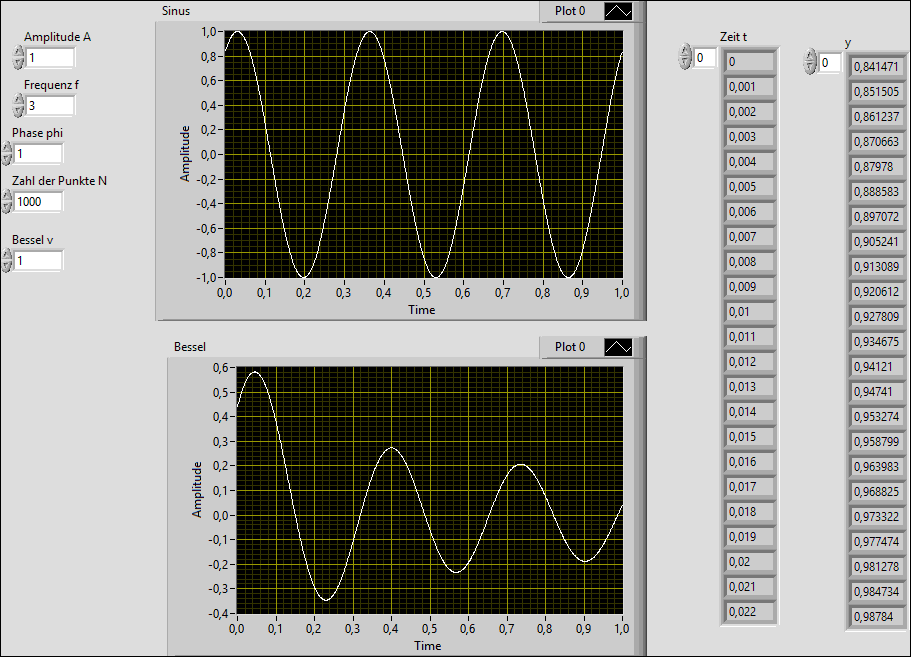
\includegraphics[width=1.0\textwidth]{EIRE2018Dateien/Tag1/sinusbessel-bilder/SinusBesselp}
		\caption{In dieser Abbildung ist das Frontpanel als Ausgabe und Benutzeroberfläche dargestellt.}
		\label{sinusbesselausgabe}
	\end{figure}

	\noindent Zusätzlich zur Sinus-Funktion wird eine Bessel-Funktion erster Gattung $J_{\nu}$ mit LabVIEW realisiert und ebenfalls in das Programm in \cref{sinusbesselprogrammcode} mit aufgenommen. Das entsprechende Blockdiagrammobjekt ist mit \glqq $J_{\nu}(x)$ Bessel\grqq\ gekennzeichnet. Die Bessel-Funktion besitzt die allgemeine Form
	
	\begin{equation}
	J_{\nu}(x) = \sum_{j=0}^{\infty}\frac{(-1)^j \cdot \left( \frac{x}{2}\right) ^{2j+\nu}}{j! \cdot \Gamma(\nu + j + 1)} \ .
	\end{equation}
	
	\noindent Wobei $\nu$ die Ordnung der Bessel-Funktion bildet, $\Gamma(\cdot)$ die Gamma-Funktion darstellt und $x$ auf Basis des Programmcodes in \cref{sinusbesselprogrammcode} als 
	
	\begin{equation}
	x := 2\pi f t + \varphi = \frac{2\pi f \cdot i}{N} + \varphi
	\end{equation}
	
	\noindent definiert ist. Der Fließkommazahlen-Wert für $\nu$ ist, ähnlich wie beim Sinus-Programm, über das entsprechende Bedienelement auf der linken Seite des Frontpanels einstellbar, was in \cref{sinusbesselausgabe} zu erkennen ist. Genauso wie beim Sinus-Programm findet die Berechnung der $x$- und $J_{\nu}(x)$-Werte innerhalb der For-Schleife statt. Die Werteausgabe erfolgt in Form eines $X$-$Y$-Diagramms, dessen Anzeigeelement im unteren Bereich der \cref{sinusbesselausgabe} ersichtlich ist und in dem $J_{\nu}(x)$ als Funktion von $x$ dargestellt ist. Zudem muss das Eingangssignal für das dazugehörige Blockdiagrammobjekt in \cref{sinusbesselprogrammcode} passend umgewandelt werden, so wie zuvor beim Sinus-Programm. 

	\begin{figure}[H]
		\centering
		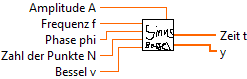
\includegraphics[width=0.5\textwidth]{EIRE2018Dateien/Tag1/sinusbessel-bilder/SinusBesselc}
		\caption{Die Abbildung zeigt das gestaltete Programm-Icon sowie die gesetzten Anschlussmöglichkeiten.}
		\label{sinusbesselicon}
	\end{figure}
	
	\noindent LabVIEW bietet die Möglichkeit ein bereits vorhandenes, selbst geschriebenes, funktionsfähiges Programm so zu bearbeiten, dass es für andere LabVIEW-Programme bzw. -Projekte als Blockdiagrammobjekt nutzbar wird. Dazu müssen zunächst die Anschlüsse festgelegt werden, sowohl die Eingänge als auch die Ausgänge. Allgemein kann es sich dabei um verschiedenste Arten von Ein-und Ausgangssignalen handeln. Bei der programmierten Sinus-Funktion verhält es sich demnach so, dass fünf Eingangs- und zwei Ausgangsanschlüsse generiert werden müssen, welche jeweils nur Gleitkommazahlen annehmen bzw. übergeben. Die Amplitude $A$, die Frequenz $f$, die Phasenverschiebung $\varphi$, die Anzahl der Punkte $N$ und die Ordnung $\nu$ der Bessel-Funktion bilden hierbei die Eingänge, die $t$-Werte sowie die $u$- bzw. $y$-Werte erscheinen über die beiden Ausgänge. Des Weiteren ist es in LabVIEW möglich das entsprechende Blockdiagrammobjekt-Icon des Programms zu gestalten. Das komplette Resultat ist in \cref{sinusbesselicon} dargestellt.
	
	\emph{Hinweis:} Aus der Betrachtung des Programmcodes in \cref{sinusbesselprogrammcode} geht hervor, dass das Blockdiagrammobjekt, welches das Array-Ausgabeelement des Frontpanels bildet und alle $u$-Werte abgreifen soll, inkorrekt eingefügt ist. Denn anstelle einer Implementierung nach der Multiplikation mit der Amplitude $A$, befindet sich das besagte Blockdiagrammobjekt davor. Sodass das Array lediglich die Werte des Ausdrucks
	
	\begin{equation}
	\sin(2\pi f t + \varphi)
	\end{equation}
	
	\noindent angibt, welche zwischen $-1$ und $1$ liegen. Da die Ausgabefunktion als Array einen erheblichen Einfluss auf das folgende Vorgehen hat, kann mit dem Sinus-Programm in dieser Form nicht weitergearbeitet werden. Im weiteren Verlauf der Projektbearbeitung ist der beschriebene Fehler allerdings behoben worden. Eine berichtigte, aktualisierte Version des Programms liegt an dieser Stelle jedoch nicht vor.
	\label{sinus_amp_fehler}
	
	\section{Lissajous-Figuren}
	
	Im Folgenden sollen je nach Werteeinstellungen auf dem Anzeigeelement der Benutzeroberfläche verschiedene Lissajous-Figuren entstehen. Dies ist in \cref{lissajous} zu sehen. Die Basis für eine solche Lissajous-Figur bilden zwei verschiedene Sinusschwingungen, welche beide dieselbe Gestalt wie die \cref{u} besitzen:
	
	\begin{equation} \label{u1u2}
	u_1(A_1,f_1,t,\varphi_1) = A_1 \cdot \sin(2\pi f_1 t + \varphi_1) \ \ \ \textnormal{und} \ \ \ u_2(A_2,f_2,t,\varphi_2) = A_2 \cdot \sin(2\pi f_2 t + \varphi_2) \ ,
	\end{equation}
	
	\noindent mit den unterschiedlichen Amplituden $A_1$ und $A_2$, den Frequenzen $f_1$ und $f_2$ sowie den Phasenverschiebungen $\varphi_1$ und $\varphi_2$. Zudem bedarf es eines zweidimensionalen kartesischen Koordinatensystems mit Rechts- und Hochachse. Eine Lissajous-Figur entsteht nun dadurch, dass man der $x$-Achse die Funktion $u_1$ und der $y$-Achse die Funktion $u_2$ zuweist. Je nachdem wie man die Werte für $A_1$, $A_2$, $f_1$, $f_2$, $\varphi_1$, $\varphi_2$ und $N$ wählt, ergeben sich dann unterschiedliche Lissajous-Figuren.
	
	\begin{figure}[H]
		\centering
		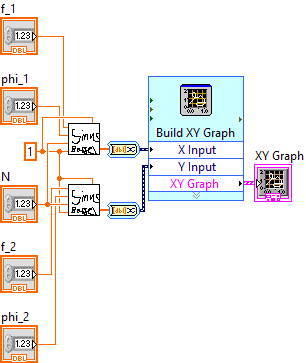
\includegraphics[width=0.6\textwidth]{EIRE2018Dateien/Tag1/lissajous-bilder/Lissajousd}
		\caption{Dargestellt ist das Blockdiagramm und der LabVIEW-Programmcode, mit dem sich Lissajous-Figuren realisieren lassen.}
		\label{lissajousprogrammcode}
	\end{figure}

	\noindent Das dazugehörige LabVIEW-Programm sowie dessen Blockdiagramm und Programmcode sind in \cref{lissajousprogrammcode} zu erkennen. Die in \cref{sinusfkt} erstellte Sinus-Funktion bildet die Grundlage, denn mit dieser lassen sich die beiden separaten Schwingungen $u_1$ und $u_2$ aus \cref{u1u2} realisieren. Dabei ist es möglich das Sinus-Programm als Blockdiagrammobjekt in den Programmcode einfügen, jeweils einmal für $u_1$ und $u_2$, was in \cref{lissajousprogrammcode} deutlich wird. An die offenen Eingangsanschlüsse müssen entsprechende, sogenannte \glqq Controler\grqq\ für die Frequenzen $f_1$ und $f_2$, für die Phasenverschiebungen $\varphi_1$ und $\varphi_2$ sowie für die Zahl der Stützstellen $N$ angeschlossen werden. Die dazugehörigen Bedien- bzw. Eingabeelemente befinden sich links auf dem Frontpanel des Programms, so wie es in \cref{lissajous} dargestellt ist. Für die Amplituden soll einfachheitshalber $A_1 = A_2 = 1$ gelten.

	\begin{figure}[H]
		\centering
		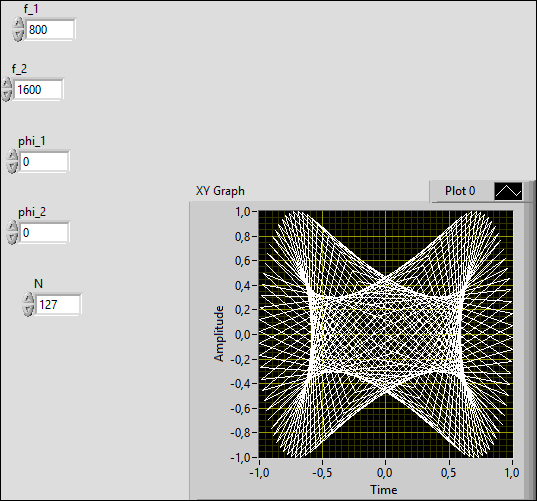
\includegraphics[width=1.0\textwidth]{EIRE2018Dateien/Tag1/lissajous-bilder/Lissajousp}
		\caption{Die Abbildung zeigt das Frontpanel bzw. die Benutzeroberfläche, in dem sich im Anzeigeelement eine Lissajous-Figur befindet. Auf der linken Seite können die entsprechenden $f_1$-, $f_2$-, $\varphi_1$-, $\varphi_2$- und $N$-Werte abgelesen werden.}
		\label{lissajous}
	\end{figure}

	\noindent An den Ausgangsanschlüssen wird ein $X$-$Y$-Diagramm angebracht, wobei die $u_1$-Werte auf der $x$-Achse und die $u_2$-Werte auf der $y$-Achse liegen. Wie beim Programm in \cref{sinusfkt}, ist dem Ausgabeelement an der entsprechenden Stelle auf der Leitung ein passendes Blockdiagrammobjekt zur Signalumwandlung vorgeschaltet. Je nach Wahl der $f_1$-, $f_2$-, $\varphi_1$-, $\varphi_2$- und $N$-Werte können sich somit die unterschiedlichsten Lissajous-Figuren formen.
	
	
	\section{Digitales Oszilloskop mit ExpressVI}
	Es wird ein Funktionsgenerator verwendet.
	Dessen Signal wird über einen Analog-Digital-Wandler durch den Computer erfasst.
	Zunächst wird das Signal in LabView mit dem entsprechenden ExpressVI verarbeitet.
	Das zugehörige Programm ist in \cref{fig_tag2_oszi_express_block} und die Frontplatte in \cref{fig_tag2_oszi_express_front} dargestellt.
	
	\begin{figure}[H]  
		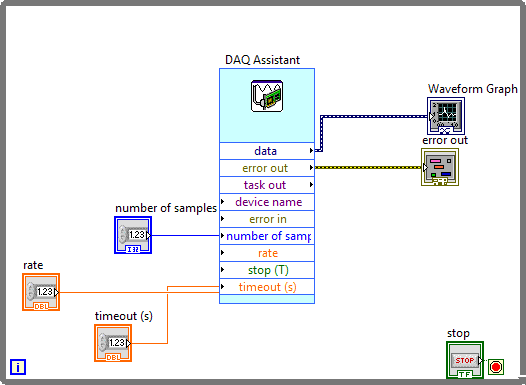
\includegraphics[width=1\textwidth]{EIRE2018Dateien/Tag2/expressVI_1d}
		\centering
		\caption{
			Einfaches Oszilloskop mithilfe des ExpressVIs zur Verarbeitung von Daten von Messgeräten.
		}
		\label{fig_tag2_oszi_express_block}
		\centering
	\end{figure}
	\begin{figure}[H]  
		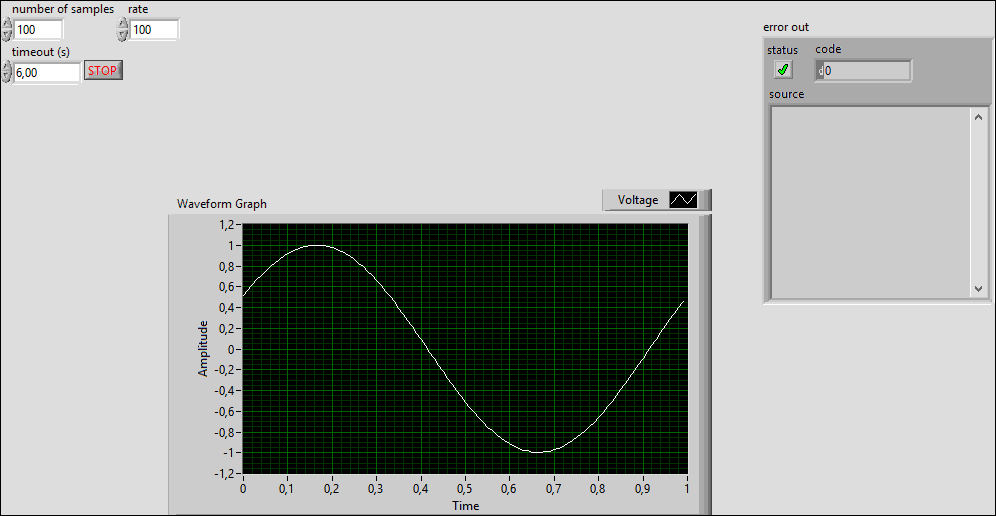
\includegraphics[width=1\textwidth]{EIRE2018Dateien/Tag2/expressVI_1p}
		\centering
		\caption{
			Frontplatte des einfachen Oszilloskop mithilfe des ExpressVIs zur Verarbeitung von Daten von Messgeräten. Dabei wurde durch den Funktionsgenerator ein sinusförmiges Signal ausgegeben.
		}
		\label{fig_tag2_oszi_express_front}
	\centering
	\end{figure}
	
	
	\section{Abtasten von Signalen}
	
	\subsection{Fouriertheorem} %kp, ob man so Theorie wiedergeben soll und ob man das mit Bindestrich schreibt.
	Gemäß des Fouriertheorems kann jede periodische Funktion als Fourierreihe bzw. Fourierintegral ausgedrückt werden.
	Dies ist nützlich bei der Zerlegung eines möglicherweise verrauschten Signals in seine Bestandteile.
	Das grundsätzliche Problem hierbei ist, dass Messprozesse immer zeitlich begrenzt ist, weshalb das Signal nicht bis in die positive und negative Unendlichkeit periodisch sein kann.
	Dies verursacht den sogenannten \enquote{Leakage-Effekt}, auf den in \cref{leakage} näher eingegangen wird.
	
	\subsection{Abtasttheorem}
	Um ein Signal abzutasten, werden im Analog-Digital-Wandler mithilfe einer Sample-and-Hold-Schaltung zeitlich diskrete Messungen durchgeführt.
	Dies lässt sich als Multiplikation des Signals mit einem Delta-Kamm ausdrücken.
	Dabei treten Summen- und Differenzfrequenzen von Abtastfrequenz und deren Oberfrequenzen mit den Frequenzen im Signal auf.
	Im Frequenzraum ergibt sich hierdurch eine periodische Fortsetzung des Spektrums des ursprünglichen Signals, wobei die Periode der Abtastfrequenz entspricht.
	Dies ist in \cref{fig_Aliasing_veranschaulichung} veranschaulicht.
	Wenn die Abtastfrequenz hinreichend groß ist, kann man nun mithilfe eines Tiefpasses das Signal herausfiltern.
	Dazu muss sie allerdings größer als das Doppelte der höchsten im Signal auftretenden Frequenz sein, da sich ansonsten das Spektrum des Signals mit den Differenzfrequenzen der nächsten Periode überlagern.
	Dies bezeichnet man als Aliasing.
	
	\begin{figure}[H]  
		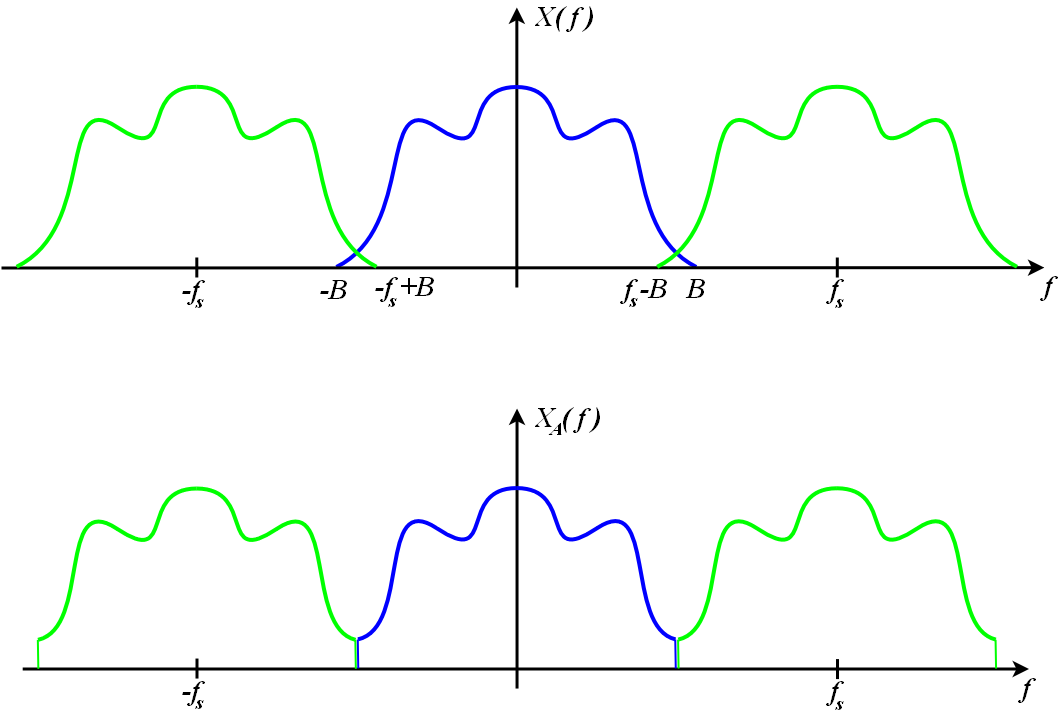
\includegraphics[width=1\textwidth]{EIRE2018Dateien/sonstige_Dateien/AliasedSpectrum}
		\centering
		\caption{
			Veranschaulichung des Effekts des Aliasing. Dargestellt ist ein Beispielsignal, das mit der Abtastfrequenz $f_S$ abgetastet wurde.
			Da diese geringer ist als das Doppelte der höchsten Frequenz im Signal $B$, überlappen sich die Perioden im Frequenzraum.
			Das ursprüngliche Signal kann durch einen Tiefpass nur unter Verlust der höheren Frequenzen rekonstruiert werden. \cite{Aliasing}
		}
		\label{fig_Aliasing_veranschaulichung}
		\centering
	\end{figure}
	
	
	%eig. zunächst Fertigstellung von Tag2 Teil 1
	\subsection{Leakage-Effekt und Fensterfunktion}
	\label{leakage}
	Wenn die Signalfrequenz kein Vielfaches des Produkts aus Abtastfrequenz und Zahl an Messpunkten pro Messung ist, tritt aufgrund der Endlichkeit des Messprozesses der sogenannte \enquote{Leakage-Effekt} auf.
	%https://de.wikipedia.org/wiki/Datei:Spectral_leakage_Sine.svg
	Dieser verursacht eine Verbreiterung des Peaks der Signalfrequenz im Frequenzbild.
	Dies ist in \cref{fig_leakage_veranschaulichung} dargestellt.
	
	\begin{figure}[H]  
		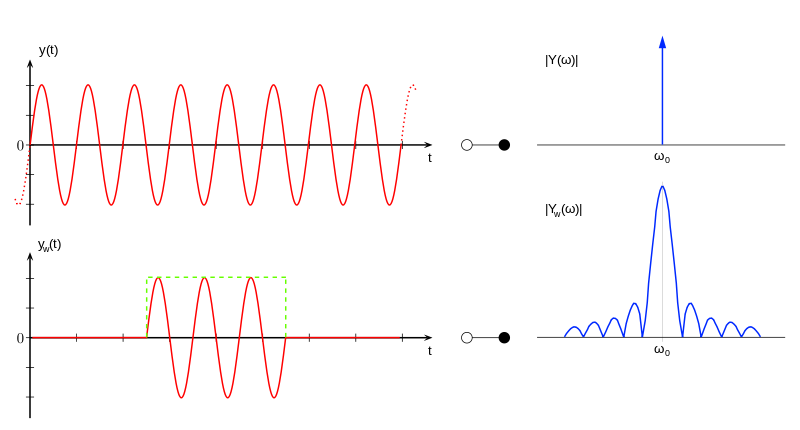
\includegraphics[width=1\textwidth]{EIRE2018Dateien/sonstige_Dateien/leakage}
		\centering
		\caption{
			Zeitlich unlimitierte (\enquote{ungefensterte}) Sinusschwingung oben und zeitlich limitierte Sinusschwingung unten (limitiert mit Rechteck-Fensterfunktion). Daneben deren Fourier-Transformierten. \cite{Leakage} %ist wörtlich übernommen, aber sollte mit dem cite ja fine sein
		}
		\label{fig_leakage_veranschaulichung}
		\centering
	\end{figure}

	Um diesen Effekt zu minimieren können Fensterfunktionen angewendet werden. %mit denen das Signal mutlipliziert wird? Wäre das immer wahr?
	Im Folgenden wird das \enquote{Von-Hann-Fenster} (auch \enquote{Hanning-Fenster}) verwendet. %mehr erklären? Hat er halt auch nicht so schöne gemacht, nur halt 1-cos
	Der Unterschied zwischen Spektralanalyse mit und ohne Von-Hann-Fenster ist in \cref{fig_tag23_oszi_manuell_front} zu erkennen, da dort ohne Fenster-Funktion zusätzliche Frequenzen in der Nähe des Peaks auftreten.
	

	\subsection{Digitales Oszilloskop ohne ExpressVI} % hier ist halt die Tagreihenfolge bissl gebrochen. Ich glaube, wir haben das an Tag 2 angefangen und Tag 3 beendet
	Das Oszilloskopprogramm von zuvor wird ersetzt durch eines, dass anstelle des ExpressVIs Konfiguration, Messung und Cleanup getrennt enthält.
	Dieses ist in \cref{fig_tag23_oszi_manuell_block} dargestellt, während in \cref{fig_tag23_oszi_manuell_front} die Frontplatte bei einem Eingangssignal von \SI{600}{\hertz}.
	
	\begin{figure}[H]  
		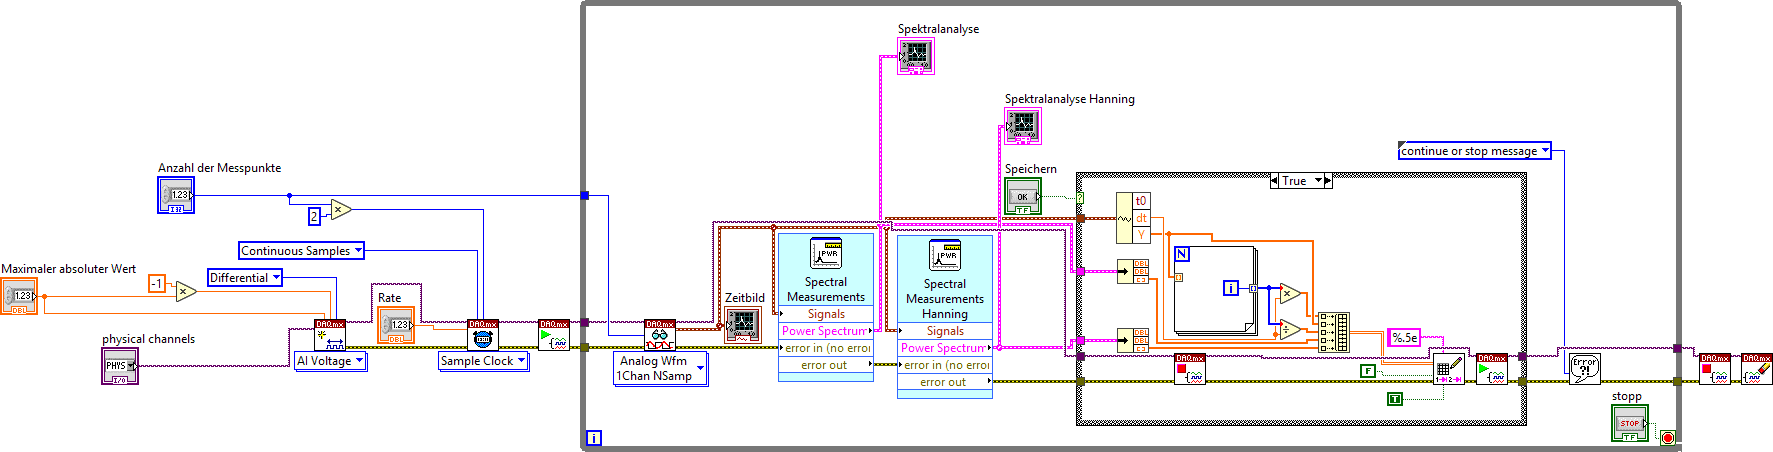
\includegraphics[width=1\textwidth]{EIRE2018Dateien/Tag3/ManuellVId}
		\centering
		\caption{
			Oszilloskopprogramm, das eine Abtastung vornimmt und das Ergebnis im Zeitbild sowie im Frequenzbild mit und ohne Hann-Fenster darstellt.
			Außerdem ist die Speicherung der Daten in einem Textdokument ermöglicht.
		}
		\label{fig_tag23_oszi_manuell_block}
		\centering
	\end{figure}

	\begin{figure}[H]  
		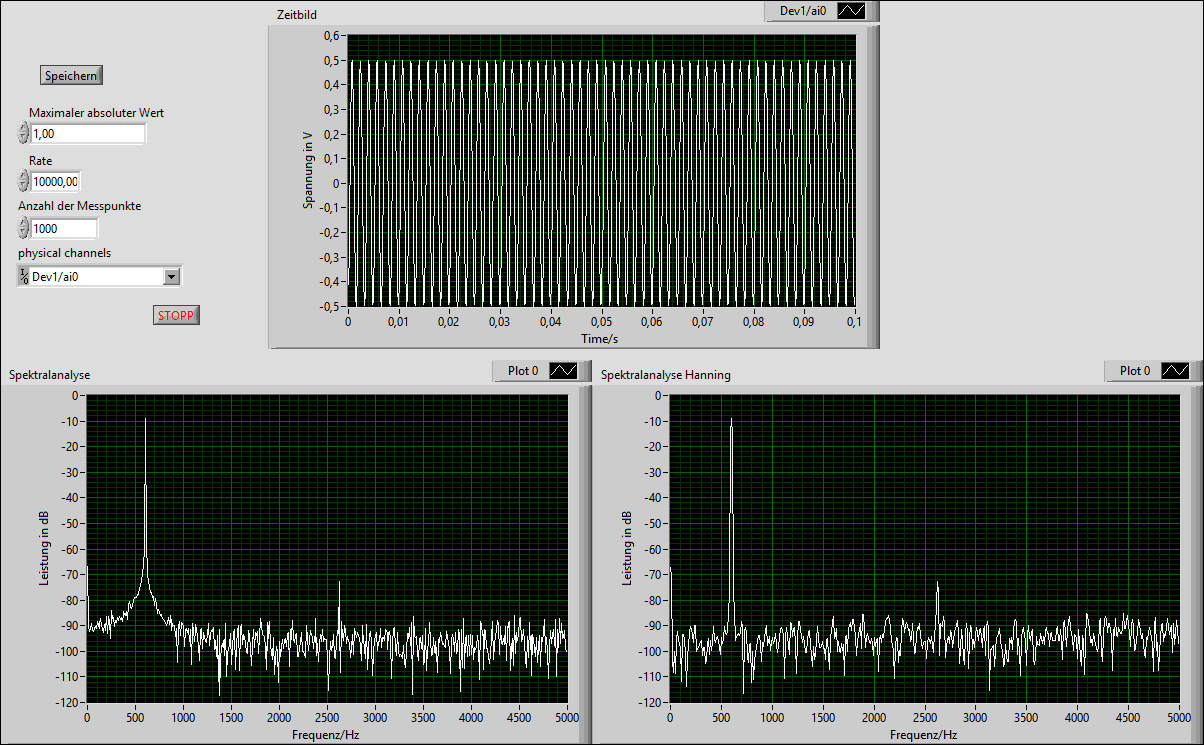
\includegraphics[width=1\textwidth]{EIRE2018Dateien/Tag3/ManuellVIp}
		\centering
		\caption{
			Oszilloskopfrontplatte. Dargestellt wird das gemessene Signal im Zeitbild sowie im Frequenzbild mit und ohne Von-Hann-Fenster. Einstellbar ist die Abtastfrequenz, die Anzahl der Messpunkte, der Eingangskanal des Messgerätes und der maximale messbare Wert, wobei der minimale auf das Negative des maximalen gesetzt wird.
			Mithilfe des Stopp-Knopfes kann das Programm gestoppt werden und mit dem Speichern-Knopf werden die aktuellen Messwerte aus allen drei Diagrammen in eine Textdatei exportiert.
		}
		\label{fig_tag23_oszi_manuell_front}
		\centering
	\end{figure}

	Hierbei wurde ebenfalls die Möglichkeit die aktuellen Messwerte zu speichern eingeführt.
	Dazu wurden die Strukturen, die in den Diagrammen dargestellt werden in ihre Bestandteile zerlegt und die Arrays der Y-Werte mit zwei Arrays für fortlaufende Zeit- und Frequenzwerte kombiniert und der Speicherfunktion zugeführt.
	Der Speichervorgang befindet sich innerhalb eines case-Konstrukts, das ignoriert wird, solange der Speichern-Knopf nicht gedrückt wurde.
	Außerdem werden Fehlermeldungen einer Fehlerdialogfunktion zugeführt, die dem Nutzer erlaubt bei Fehlern wahlweise das Programm anzuhalten oder weiterlaufen zu lassen.
	Um ein Volllaufen des Mess-Buffers zu vermeiden, wird dieser doppelt so groß wie die Anzahl der Messpunkte pro Zyklus gewählt.
	
	\subsection{Aliasing}
	Um den Effekt des Aliasings absichtlich herbeizuführen, werden bei einer Abtastfrequenz von \SI{1000}{\hertz} zwei verschiedene Signale abgetastet.
	Da bei dieser Abtastfrequenz die höchste Frequenz im Signal kleiner als \SI{500}{\hertz} sein muss, ist hierbei zu erwarten, dass ein Signal von \SI{400}{\hertz} korrekt abgetastet wird, während eines mit \SI{600}{\hertz} falsch abgetastet wird.
	Das Spektrum des abgetasteten Signals bei diesen beiden Signalfrequenzen ist in \cref{fig_ali} dargestellt.
	
	\begin{figure}[H]
		\centering
		\begin{subfigure}[t]{0.5\textwidth}
			\centering
			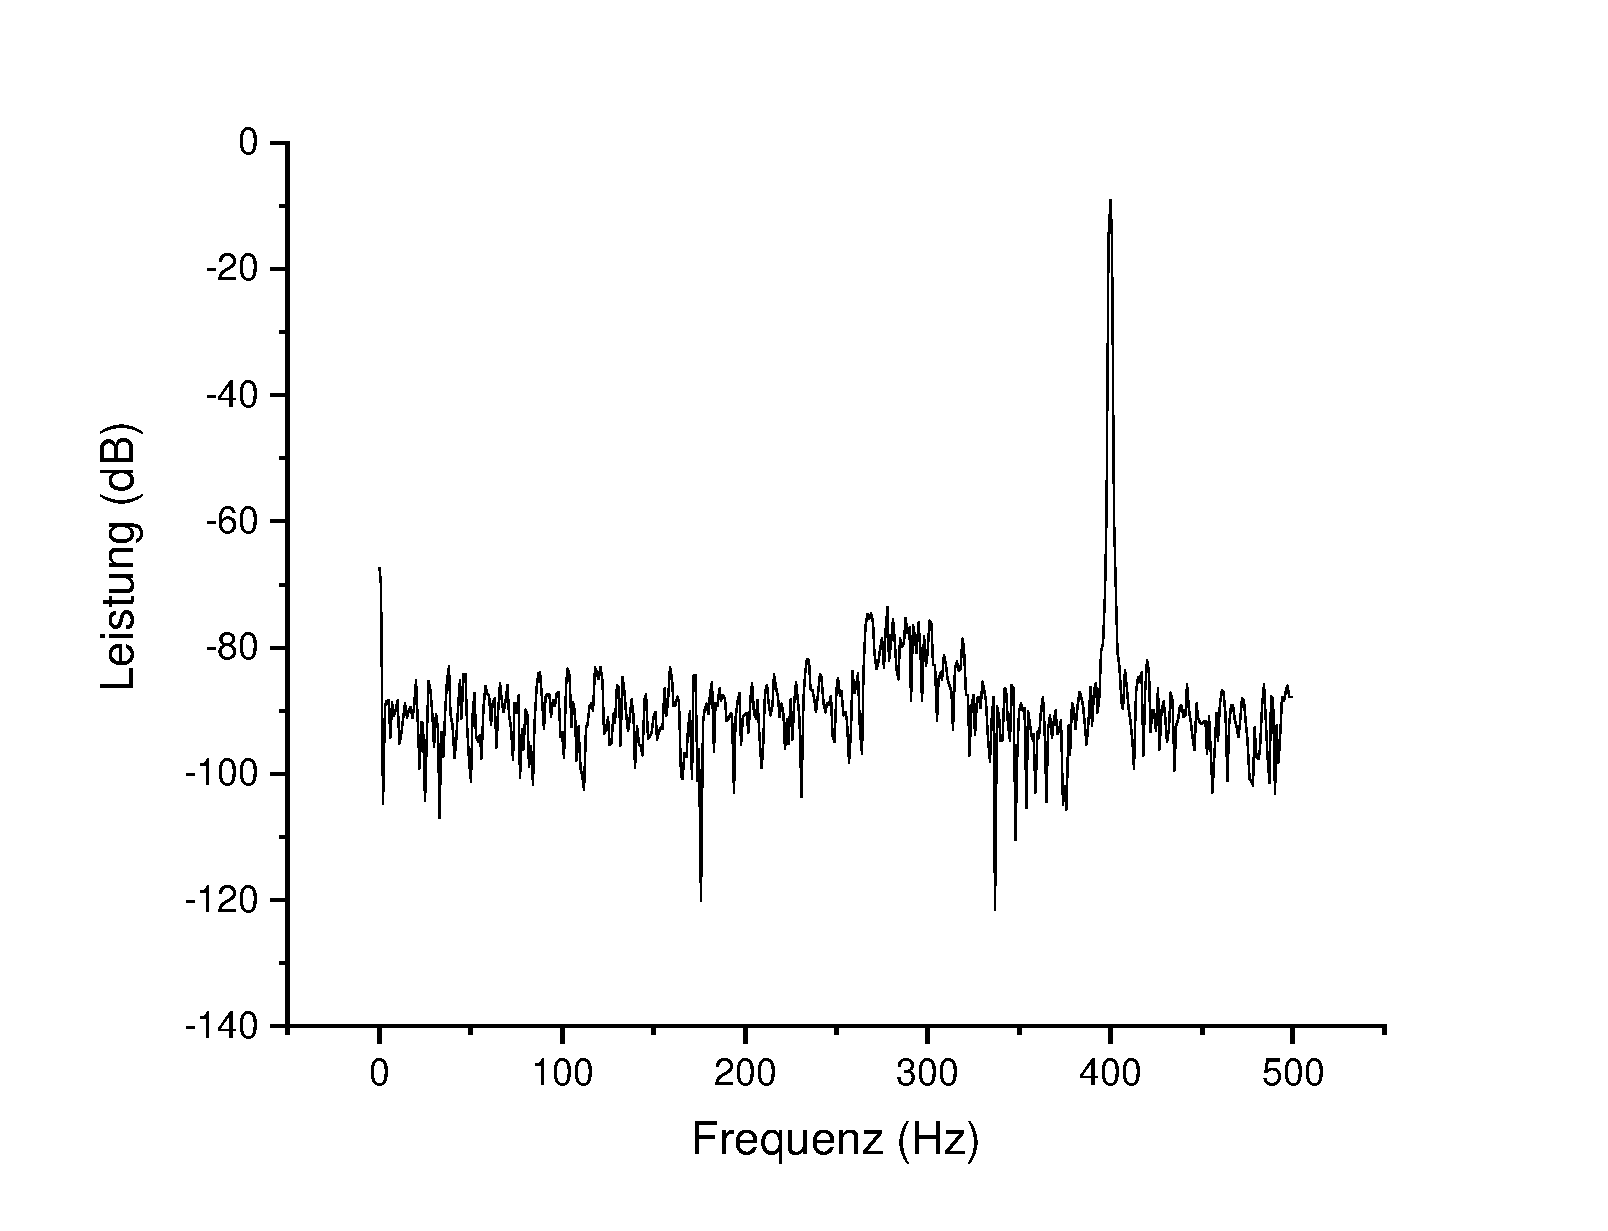
\includegraphics[width=1\textwidth]{Origin-Files/aliasing_abtast1000bei400sig}
			\caption{\SI{400}{\hertz}}
		\end{subfigure}%
		\begin{subfigure}[t]{0.5\textwidth}
			\centering
			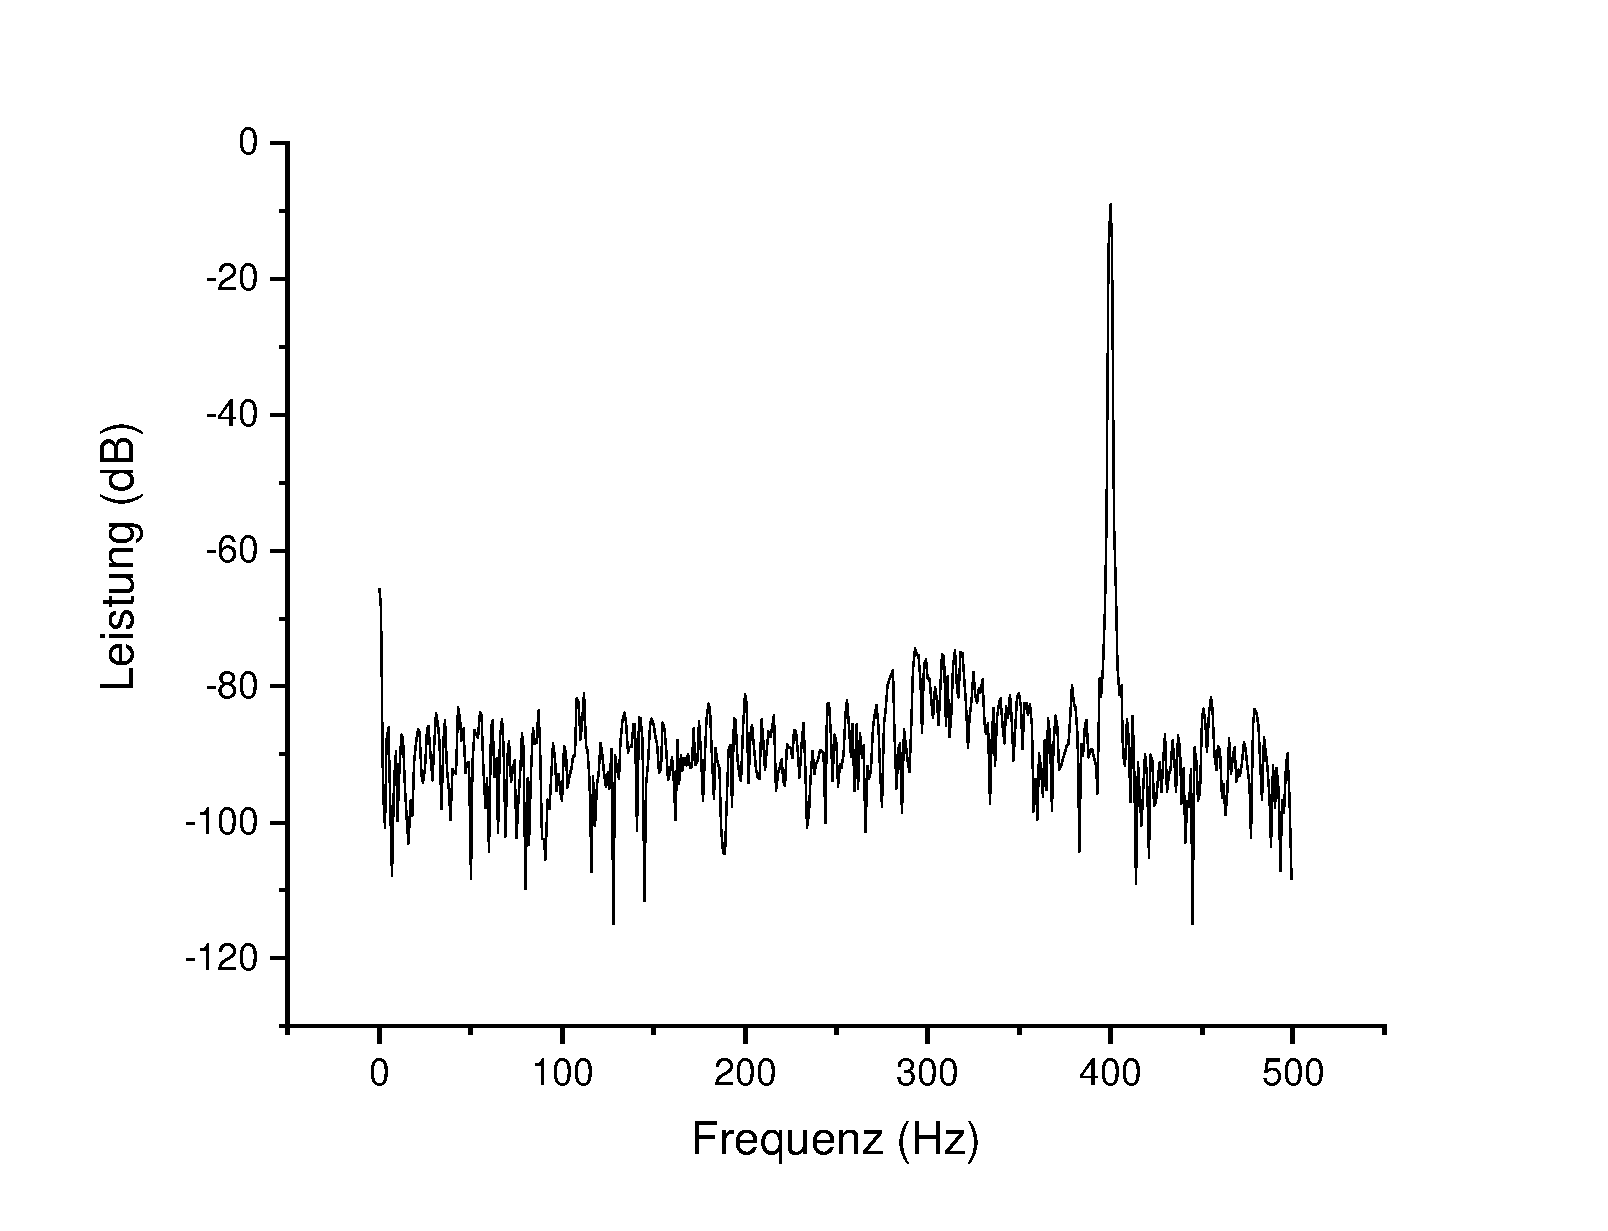
\includegraphics[width=1\textwidth]{Origin-Files/aliasing_abtast1000bei600sig}
			\caption{\SI{600}{\hertz}}
		\end{subfigure}
		\label{fig_ali}
		\caption{Mit einer Abtastfrequenz von \SI{1000}{\hertz} abgetastete Signale, deren Frequenz einmal \SI{400}{\hertz} und einmal \SI{600}{\hertz} beträgt, sodass einmal korrekt und einmal falsch abgetastet wird. Um die Sichtbarkeit zu verbessern und die übliche Oszilloskop-Optik zu erreichen, wurden die Messpunkte hier und in den folgenden Darstellungen mit einer Linie verbunden.} %TODO letzten Satz approven und sicherstellen, dass du den nicht außerhalb einer caption haben willst.
		\centering
	\end{figure}
	
	Es fällt auf, dass sich zwischen diesen beiden Signalen kein Unterschied erkennen lässt.
	Dies liegt daran, dass bei einer Signalfrequenz von \SI{600}{\hertz} die eigentliche Signalfrequenz nicht mehr vom idealen Tiefpass übertragen wird, während die Differenzfrequenz von Abtastfrequenz und Signalfrequenz \SI{400}{\hertz} beträgt.
	Es ist an den beiden Signalen zu erkennen, dass sich ein falsch abgetastetes Signal nicht mehr von einem korrekt abgetasteten Signal bei der entsprechenden Differenzfrequenz unterscheiden lässt.
	Man stellt fest, dass man vor der Abtastung bereits wissen muss, welche Frequenzen im Signal vorkommen. 
	
	\subsection{Unpassende Abtastrate}
	Zusätzlich zu den zuvor genannten Effekten kann bei der Abtastung von Signalen noch ein weiterer Effekt auftreten, der im Folgenden kurz beleuchtet werden soll.
	Dabei wird das Produkt aus Abtastfrequenz und Anzahl der Messpunkte pro Messdurchgang als \enquote{Abtastrate} bezeichnet. %Anführungsstriche gut?
	Wenn die Signalfrequenz kein Vielfaches der Abtastrate ist, führt dies dazu, dass eine eigentlich scharfe Frequenz im Spektrum unscharf wird und Frequenzen geringerer Intensität in der Nähe dieser überdeckt werden.
	%Er hat das leider sehr schlecht erklärt und keinerlei Fachbegriffe verwendet, die man hier aufgreifen könnte. Und im Internet hab ich auch nichts zu dem Effekt gefunden, weshalb ich dann halt meine Worte genutzt habe.
	Auch dies wird absichtlich herbeigeführt und in \crefrange{fig_tag3_unpassend_230hz}{fig_tag3_unpassend_235hz} dargestellt.
	Hierbei beträgt die Abtastfrequenz \SI{1000}{\hertz} und die Anzahl der Messpunkte pro Messdurchgang \num{100}, woraus sich eine Abtastrate von \SI{10}{\hertz} ergibt.
	
	\begin{figure}[H]  
		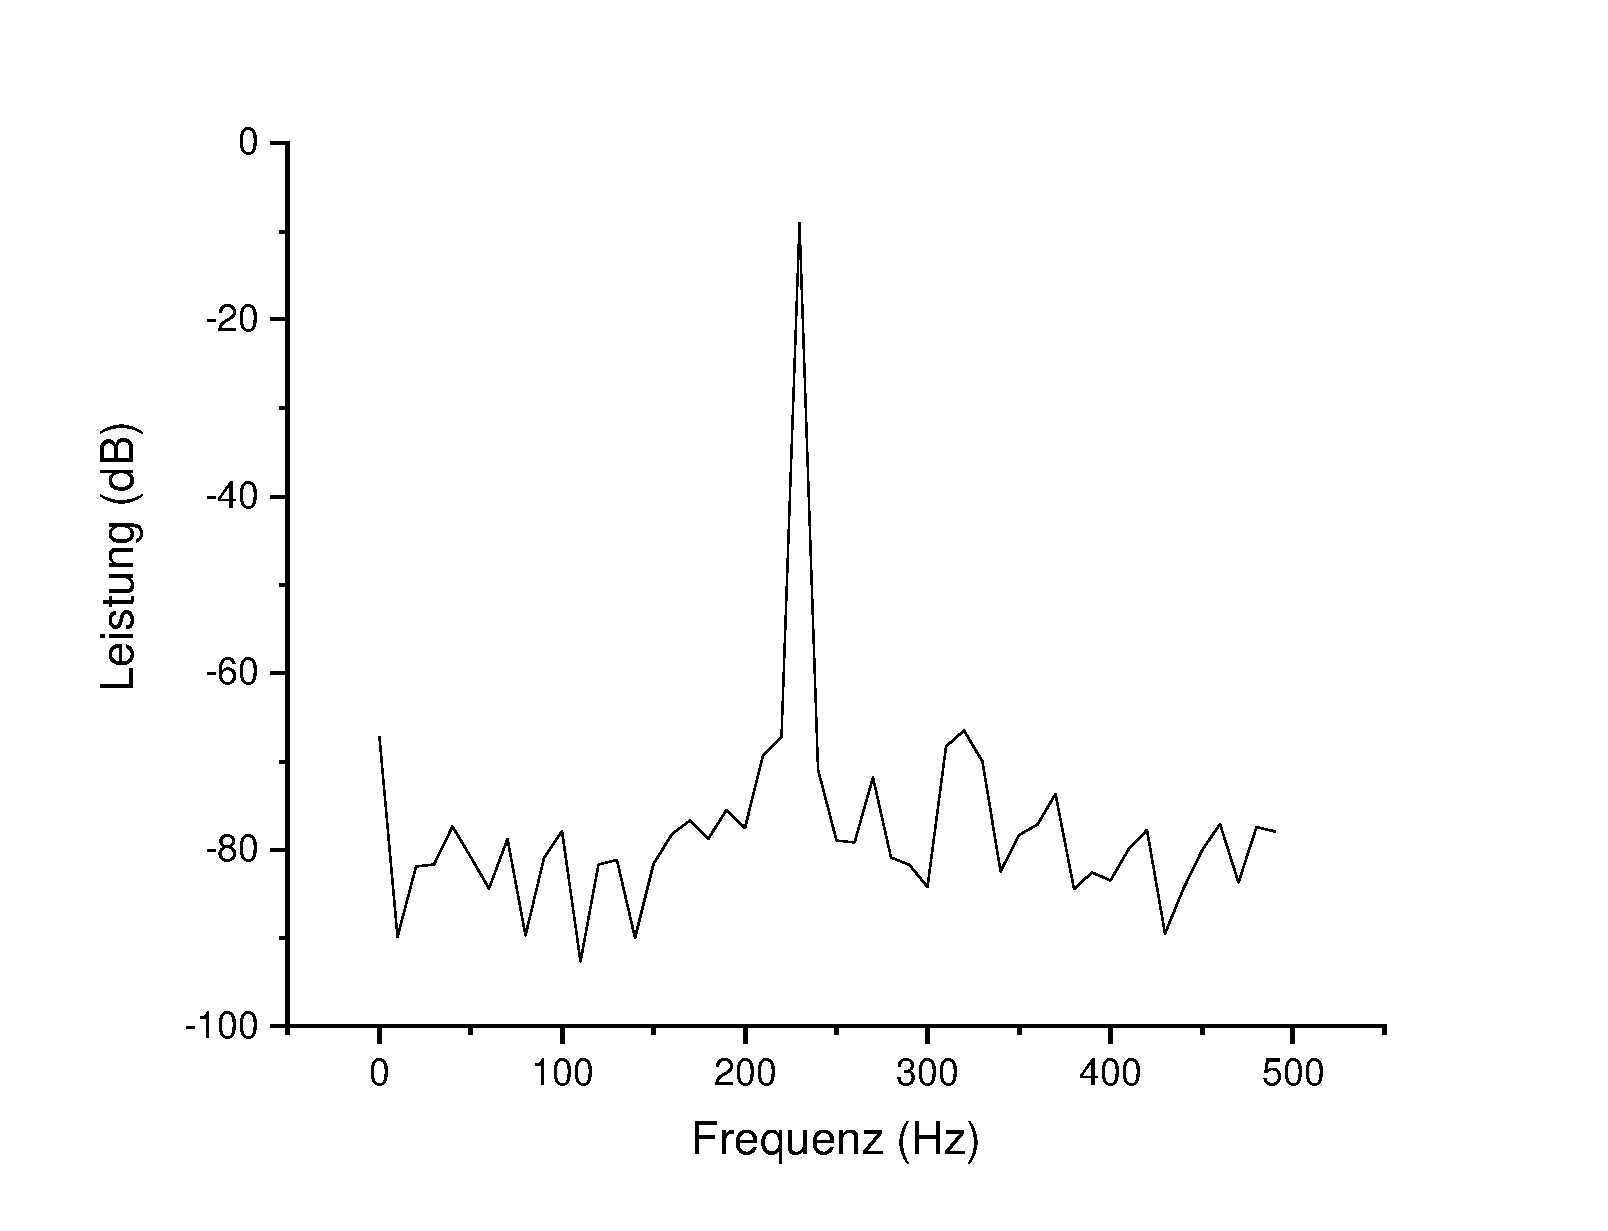
\includegraphics[width=0.5\textwidth]{Origin-Files/unpassend_230nonhann}
		\centering
		\caption{
			Spektrum eines Signals mit einer Frequenz von \SI{230}{\hertz}, was ein Vielfaches der Abtastrate ist, weshalb hier die Signalfrequenz scharf zu erkennen ist.
		}
		\label{fig_tag3_unpassend_230hz}
		\centering
	\end{figure}
	
	\begin{figure}[H]  
		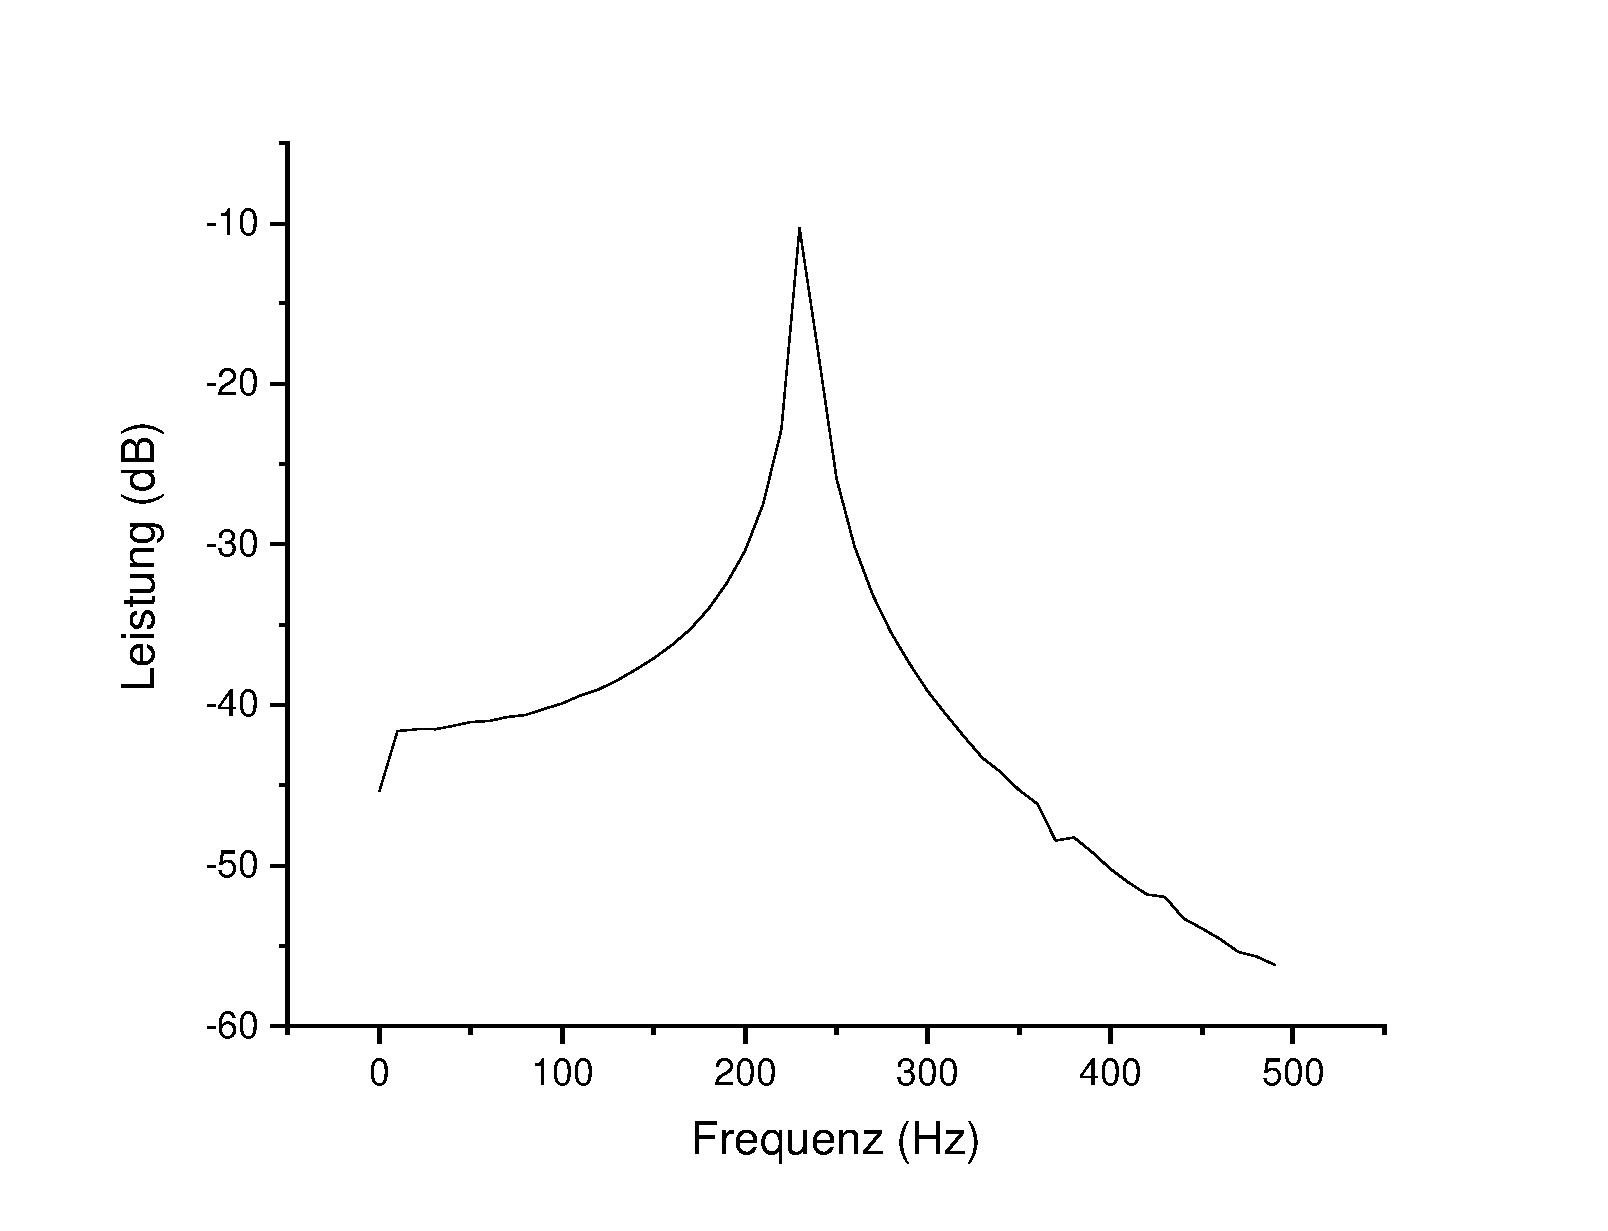
\includegraphics[width=0.5\textwidth]{Origin-Files/unpassend_233nonhann}
		\centering
		\caption{
			Spektrum eines Signals mit einer Frequenz von \SI{233}{\hertz}, was kein Vielfaches der Abtastrate ist, weshalb hier zu erkennen ist, dass die Signalfrequenz unscharf wird.
		}
		\label{fig_tag3_unpassend_233hz}
		\centering
	\end{figure}
	
	\begin{figure}[H]  
		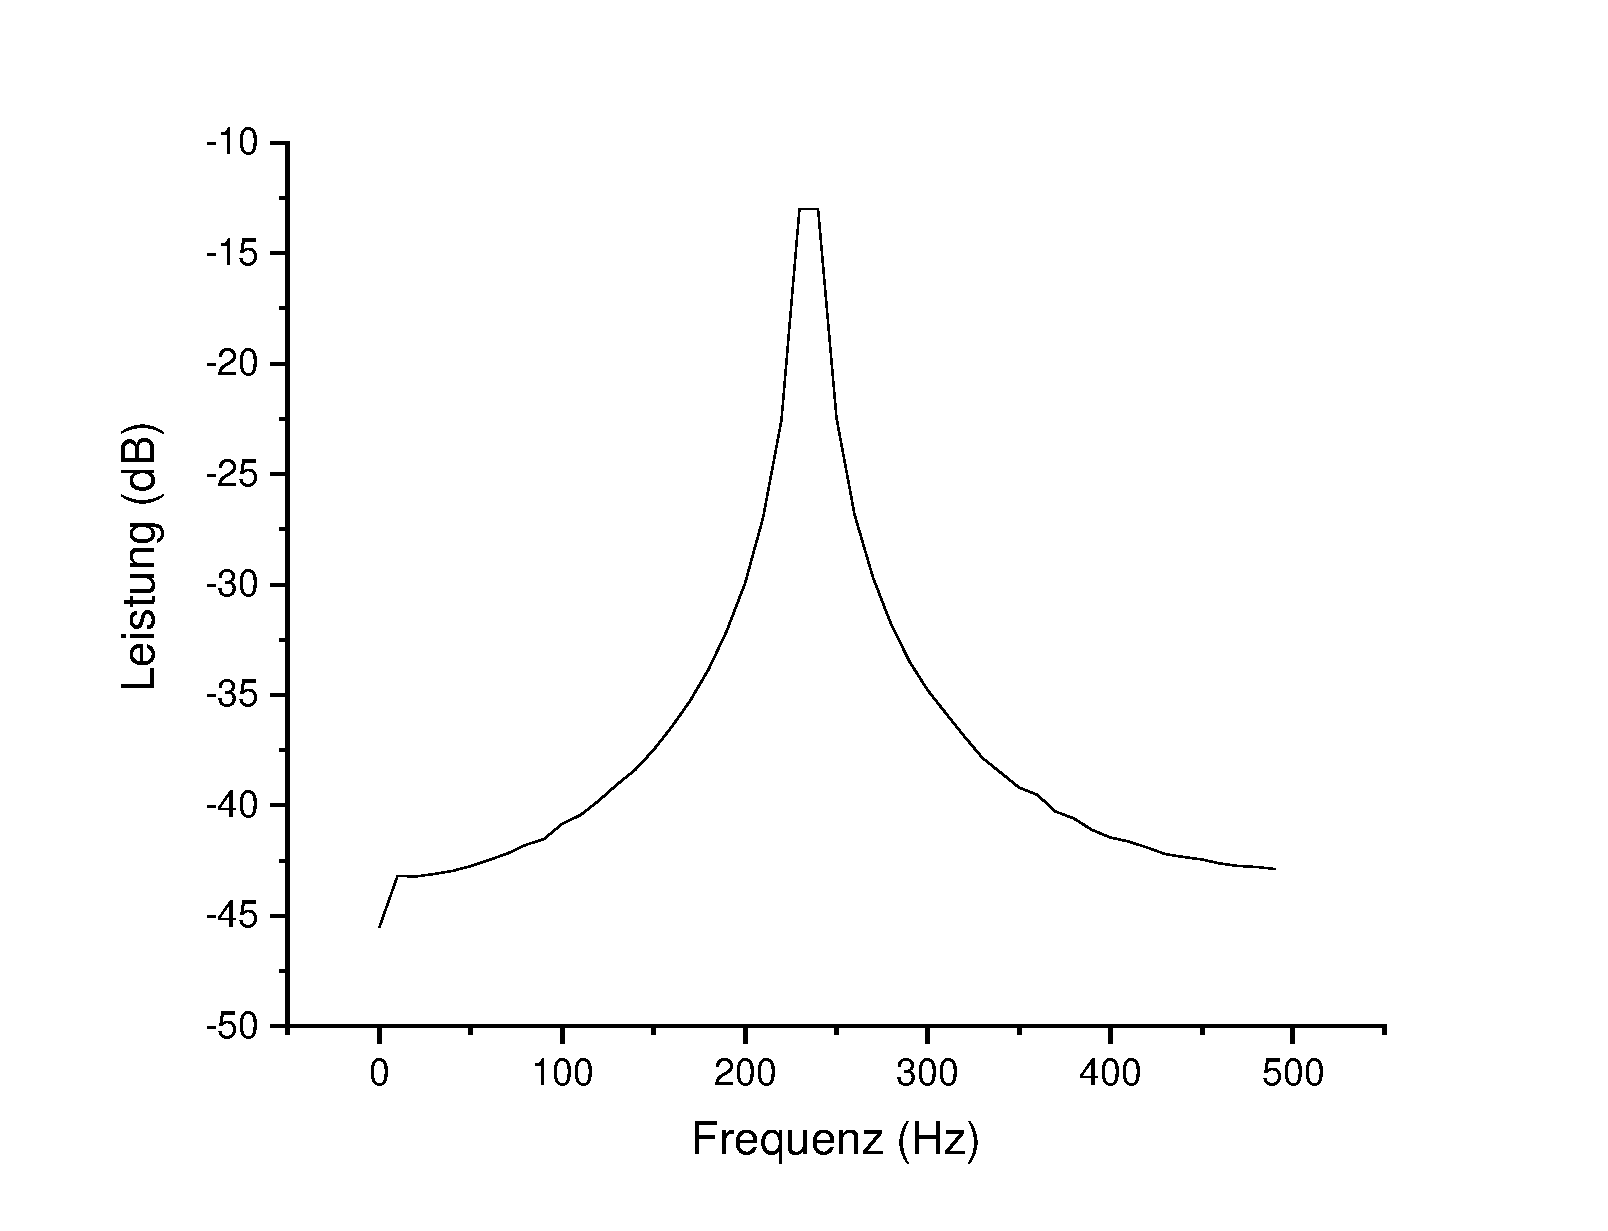
\includegraphics[width=0.5\textwidth]{Origin-Files/unpassend_235nonhann}
		\centering
		\caption{
			Spektrum eines Signals mit einer Frequenz von \SI{235}{\hertz}, was kein Vielfaches der Abtastrate ist, weshalb hier zu erkennen ist, dass die Signalfrequenz unscharf wird.
		}
		\label{fig_tag3_unpassend_235hz}
		\centering
	\end{figure}

	
	\section{Amplitudenmodulierte Signale}

	\subsection{Erzeugung eines amplitudenmodulierten Signals} \label{AMSignalErzeugung}
	
	Es soll nun ein amplitudenmoduliertes Signal (auch als AM-Signal bezeichnet) erzeugt werden und über die Soundkarte des verwendeten PCs ausgegeben werden.
	Dabei wird das Signal der Soundkarte wieder auf den Analog-Digital-Wandler gegeben und mit dem zuvor erstellten Oszilloskopprogramm verarbeitet.
	In \cref{fig_tag3_am_soundkarte_block} ist das dazu verwendete LabView-Programm dargestellt.
	Moduliert werden soll die Überlagerung zweier Signale mit einstellbarer Frequenz und Amplitude.
	Auch Trägerfrequenz und Modulationsgrad soll einstellbar sein.
	Die Amplitudenmodulation lässt sich durch die Gleichung
	\begin{equation} \label{AMFormel}
		S_{AM}(t)=S_T (1+m \cdot s(t)) \cdot \cos(2\pi f_T t)
	\end{equation}
	beschreiben.
	Da die Überlagerung von zwei sinusförmigen Signalen beliebiger aber fester Frequenz moduliert werden soll gilt:
	\begin{equation} \label{Ursprungssignal}
		s(t) = A_1 \cos (2\pi f_1 t) + A_2 \cos (2\pi f_2 t) \ . 
	\end{equation}
	
	Diese beiden Gleichungen sollen im Folgenden durch Operationen auf Arrays realisiert und als Audiosignal ausgegeben werden.	
	Dazu wird das in \cref{sinusfkt} erstellte Programm verwendet, um Arrays von Sinusfunktionen zu erstellen.
	Diesem wird in jedem Fall die Phase $0$ zugeführt und $44100$ Stützstellen gewählt, weil dies der Abtastrate bei CDs entspricht.
	Dem Programm wird zunächst eine Amplitude von $1$ gegeben und dann werden alle Array-Elemente mit der gewählten Amplitude multipliziert.
	Dies hängt lediglich damit zusammen, dass zuvor im Sinus-erstellenden Programm ein Fehler vorhanden war, der dies nötig machte (vgl. \cref{sinus_amp_fehler}).
	In \cref{fig_tag3_am_soundkarte_block} ist zu erkennen, dass zunächst zwei Sinus-Arrays erstellt werden, für die jeweils eine Signalfrequenz und -amplitude gewählt werden.
	Die beiden resultierenden Arrays werden addiert, mit dem Modulationsgrad multipliziert und dann mit dem Array der Trägerfrequenz multipliziert.
	Dieses wurde zuvor in gleicher Art und Weise mit dem Sinus-Programm bei der einstellbaren Trägerfrequenz erstellt.
	Für die Amplitude des Trägersignals wird der Kehrwert der maximalen Signalamplitude gewählt, damit die resultierende Amplitude immer auf $1$ liegt, da die Soundkarte höhere Werte nicht verarbeitet.
	Das resultierende Array wird im Zeit- und Frequenzbild dargestellt und dann mithilfe der entsprechenden VIs über die Soundkarte ausgegeben. %TODO sicherstellen, dass vorher irgendwo steht dass VI für visual instrument oder so steht.
	Hierfür wird die Abtastrate von \SI{44100}{\hertz}, die Anzahl der Kanäle von $1$ eingestellt und der Modus \enquote{Continuos Samples} gewählt, da das Signal fortlaufend erzeugt werden soll.
	Außerdem wird das Element zur Ausgabe von Fehlern verwendet, dass es erlaubt, das Programm beim Auftreten von Fehlern wahlweise zu beenden oder weiterlaufen zu lassen und das Signal in jedem Schleifendurchlauf 
	
	\begin{figure}[H]  
		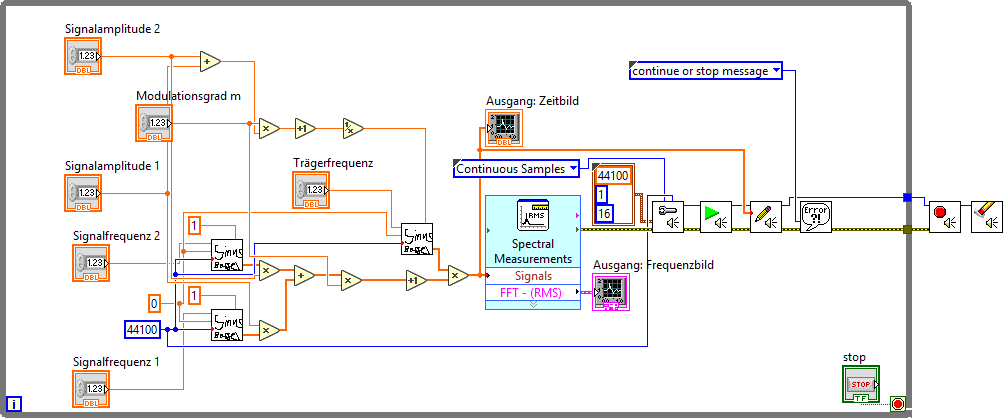
\includegraphics[width=1\textwidth]{EIRE2018Dateien/Tag3/Soundkarteoutoszi/AMd}
		\centering
		\caption{
			Blockdiagramm des Programms zur Erzeugung eines amplitudenmodulierten Signals und Ausgabe dessen über die Soundkarte.
		}
		\label{fig_tag3_am_soundkarte_block}
		\centering
	\end{figure}
	
	\begin{figure}[H]  
		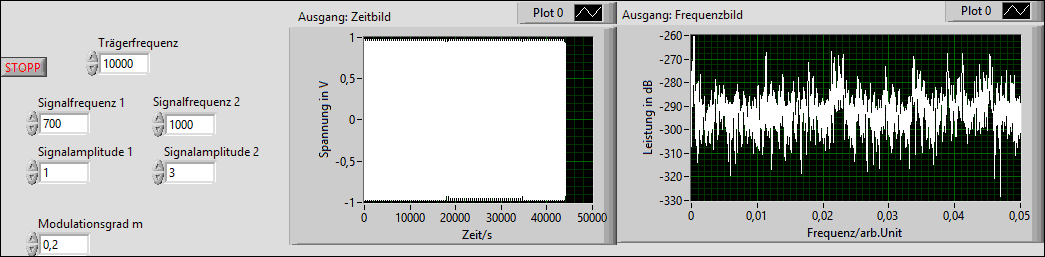
\includegraphics[width=1\textwidth]{EIRE2018Dateien/Tag3/Soundkarteoutoszi/AMp}
		\centering
		\caption{
			Frontplatte des Programms zur Erzeugung eines amplitudenmodulierten Signals und Ausgabe dessen über die Soundkarte.
		}
		\label{fig_tag3_am_soundkarte_front}
		\centering
	\end{figure}

	
\iffalse %auskommentiert weil ergibt keinen Sinn und ist eh später zu sehen.
	\begin{figure}[H]
		\centering
		\begin{subfigure}[t]{0.5\textwidth}
			\centering
			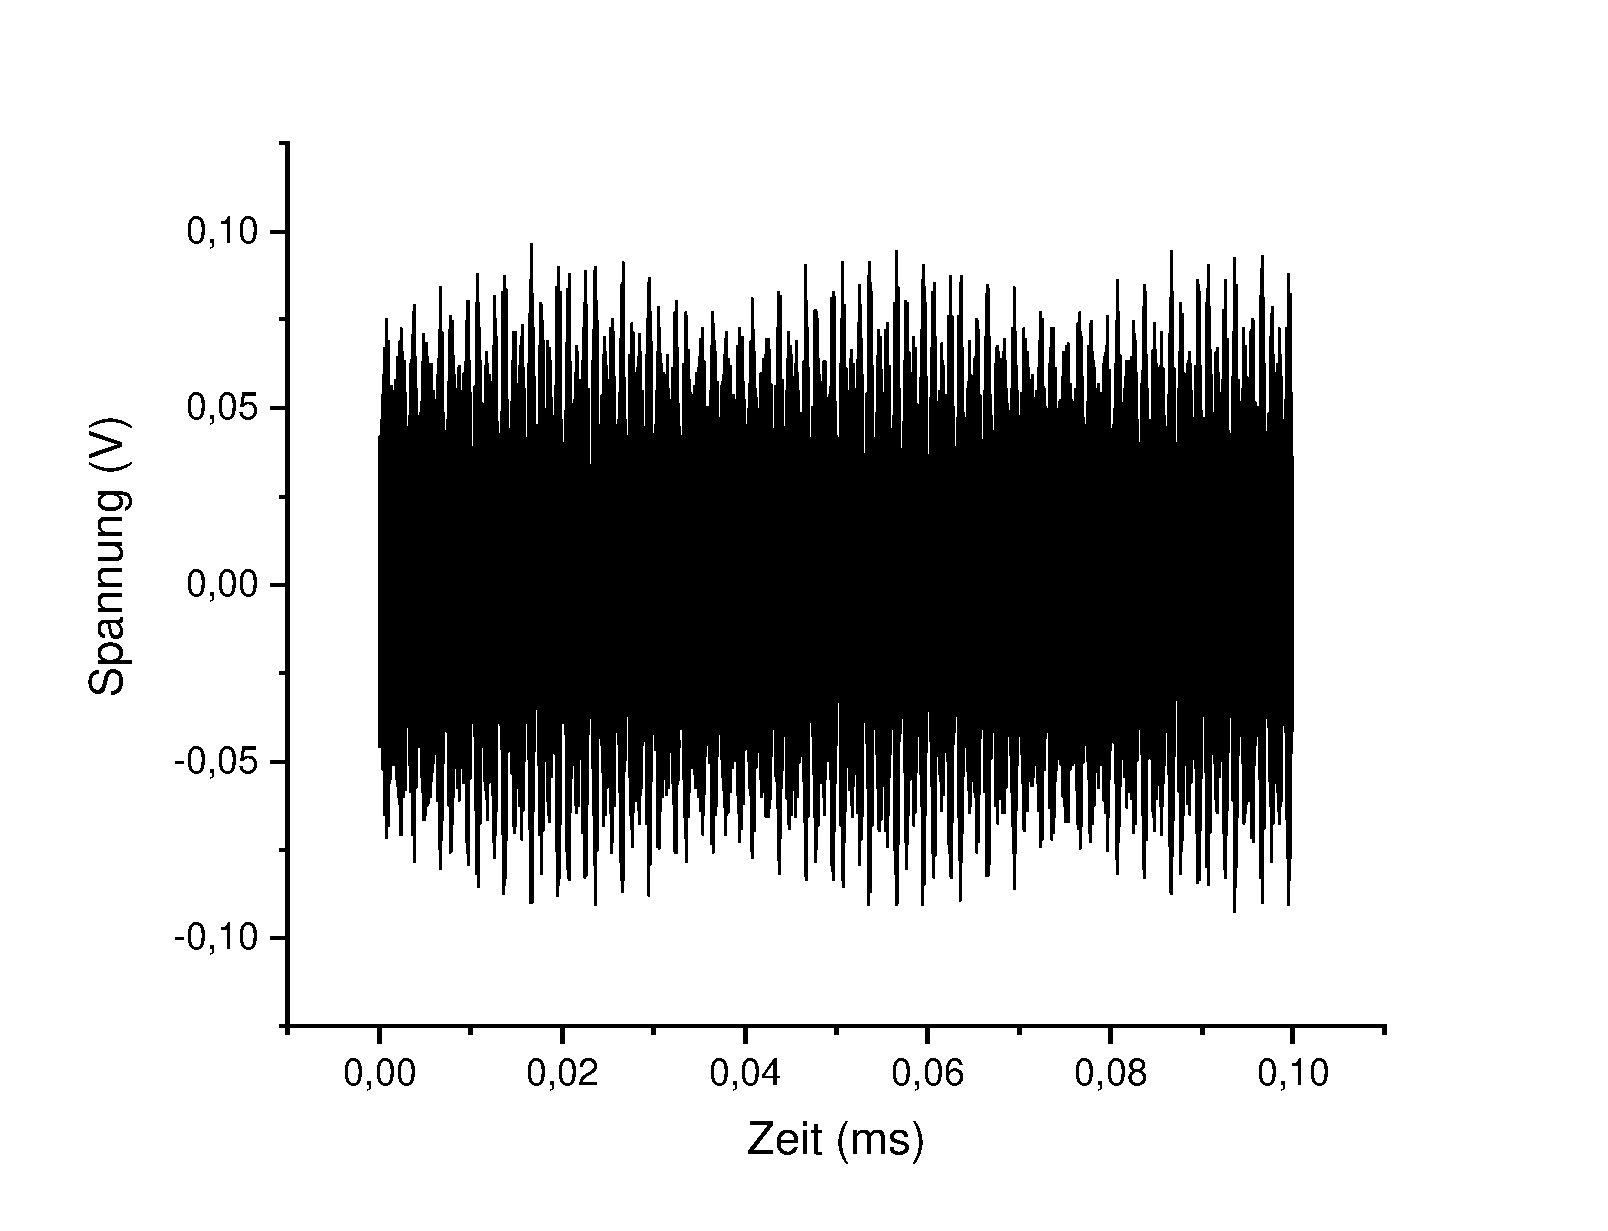
\includegraphics[width=1\textwidth]{Origin-Files/AM-Zeit}
			\caption{Zeitdomäne}
		\end{subfigure}%
		\begin{subfigure}[t]{0.5\textwidth}
			\centering
			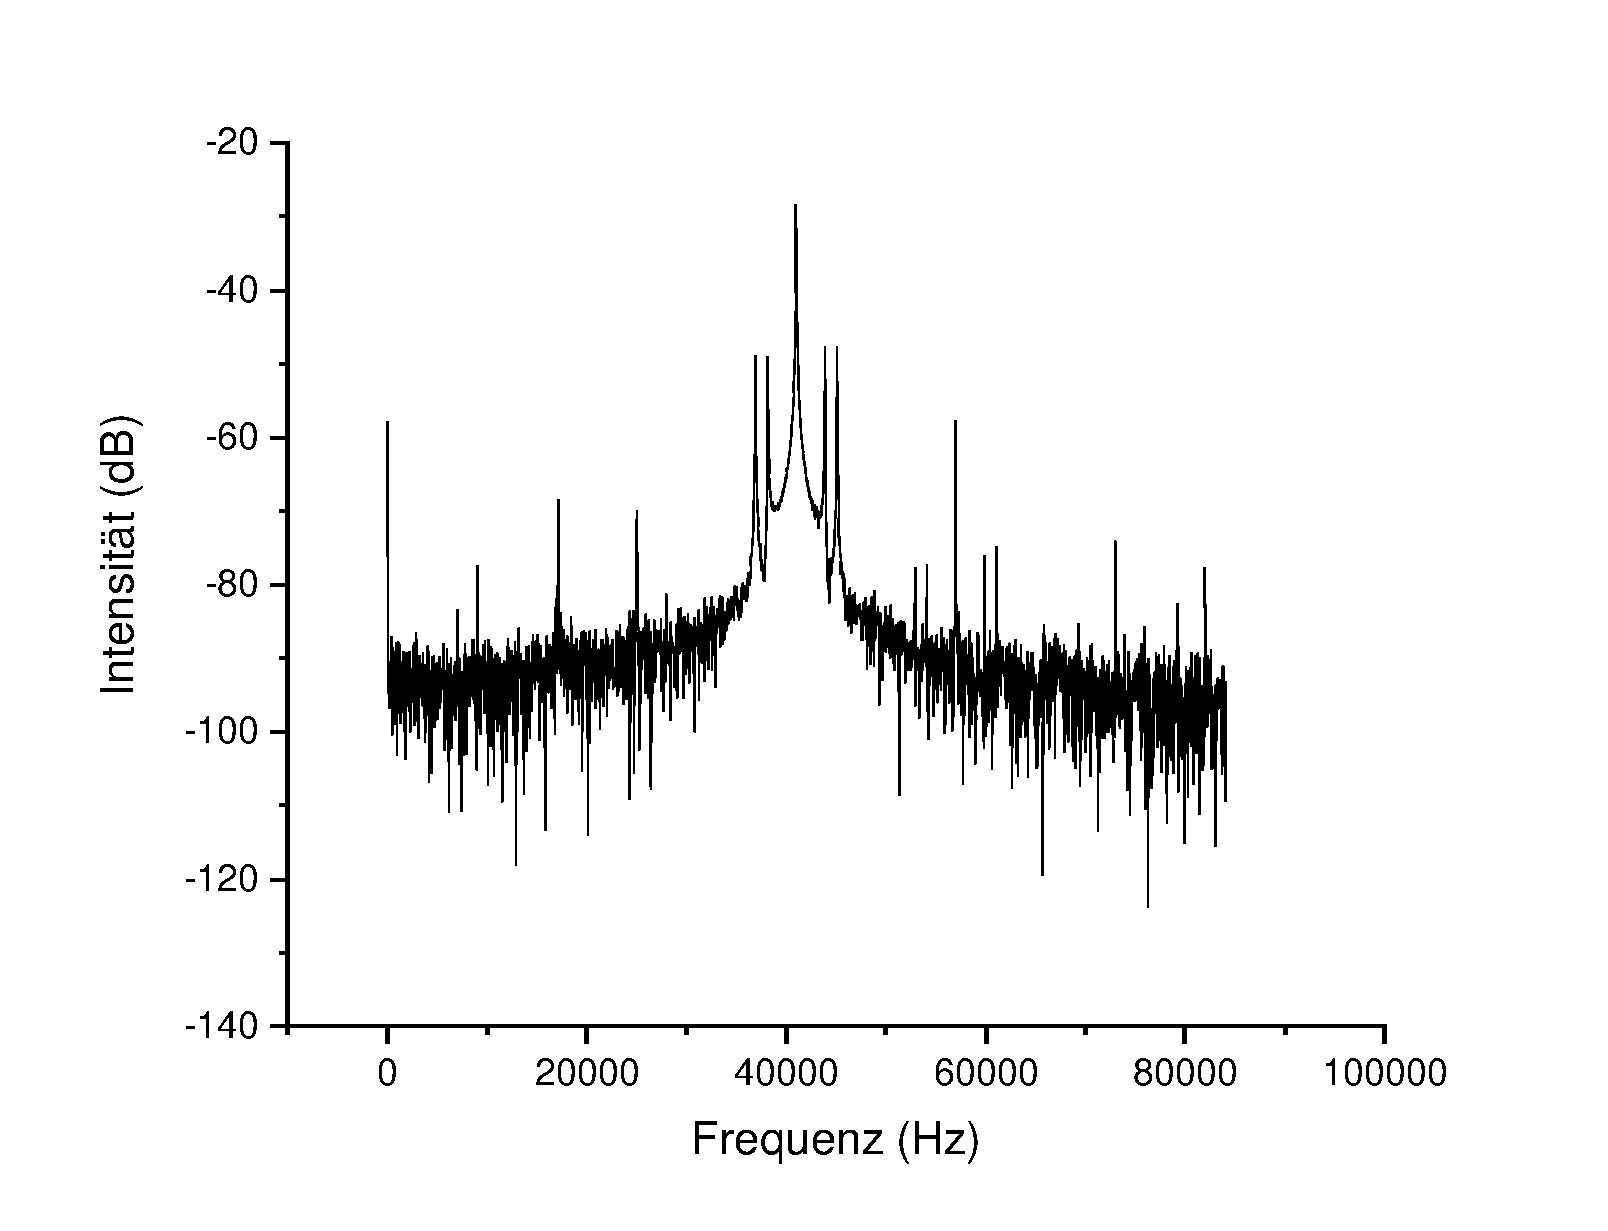
\includegraphics[width=1\textwidth]{Origin-Files/AM-Freq-Hann}
			\caption{Frequenzdomäne}
		\end{subfigure}
		\label{fig_tag3_am_soundkarte}
		\caption{Ausgabe des Oszilloskopprogramms in der Zeit- und Frequenzdomäne bei Erfassung des amplitudenmodulierten Signals, das mittels der Soundkarte ausgegeben wird.}
		\centering
	\end{figure}
\fi

	Auf das Ergebnis der Modulation wird im folgenden Abschnitt eingegangen.
	
	%Rausgenommen, weil komisch und nicht wichtig:
	%In der Frequenzdomäne lässt sich hier erkennen, dass die eingestellte Trägerfrequenz von %TODO hart komisch
	%Darüber hinaus ist zu sehen, dass einige zusätzliche Frequenzen erheblicher Leistung auftreten.
	%Diese lassen sich nur durch Störeffekte bei der Erzeugung des Signals durch die Soundkarte erklären. %und theoretisch durch Erfassung, halte ich halt für unwahrscheinlicher
	

	\subsection{Demodulation eines AM-Signals durch Quadrieren und Betragsbildung} \label{DemodulationAM}
	%Betrag, Quadrat
	Um nun das amplitudenmodulierte Signal im Oszilloskopprogramm wieder demodulieren zu können, wird ein Case-Konstrukt eingeführt, welches nach Auswahl des Benutzers wahlweise das Signal nicht demoduliert, mit sich selbst multipliziert oder den Betrag des Signals bildet, da in den letzten beiden Fällen unter anderem wieder die Ursprungsfrequenzen vorliegen.
	Nach diesem Schritt wird das Signal im Zeit- und Frequenzbild dargestellt und danach zusätzlich durch einen Tiefpass geführt, der auftretende höhere Frequenzen herausfiltert, und dann erneut im Zeit- und Frequenzbild dargestellt.
	Außerdem wird die Speicherung von zuvor erweitert, sodass das Signal vor der Demodulation, vor dem Tiefpass und nach diesem gespeichert werden kann.
	Das fertige Programm ist in \cref{fig_tag3_am_demod_block} und die zugehörige Frontplatte in \cref{fig_tag3_am_demod_front} dargestellt.
	Dass man in letzterem anhand der Zeitdomäne wenig erkennen kann, liegt an der Vielzahl und der Größe der auftretenden Frequenzen.
	Diese Tatsache gilt für alle der kommenden Untersuchungen, weshalb im Folgenden nur noch die Frequenzdomäne dargestellt werden wird.
	

	\begin{figure}[H]  
		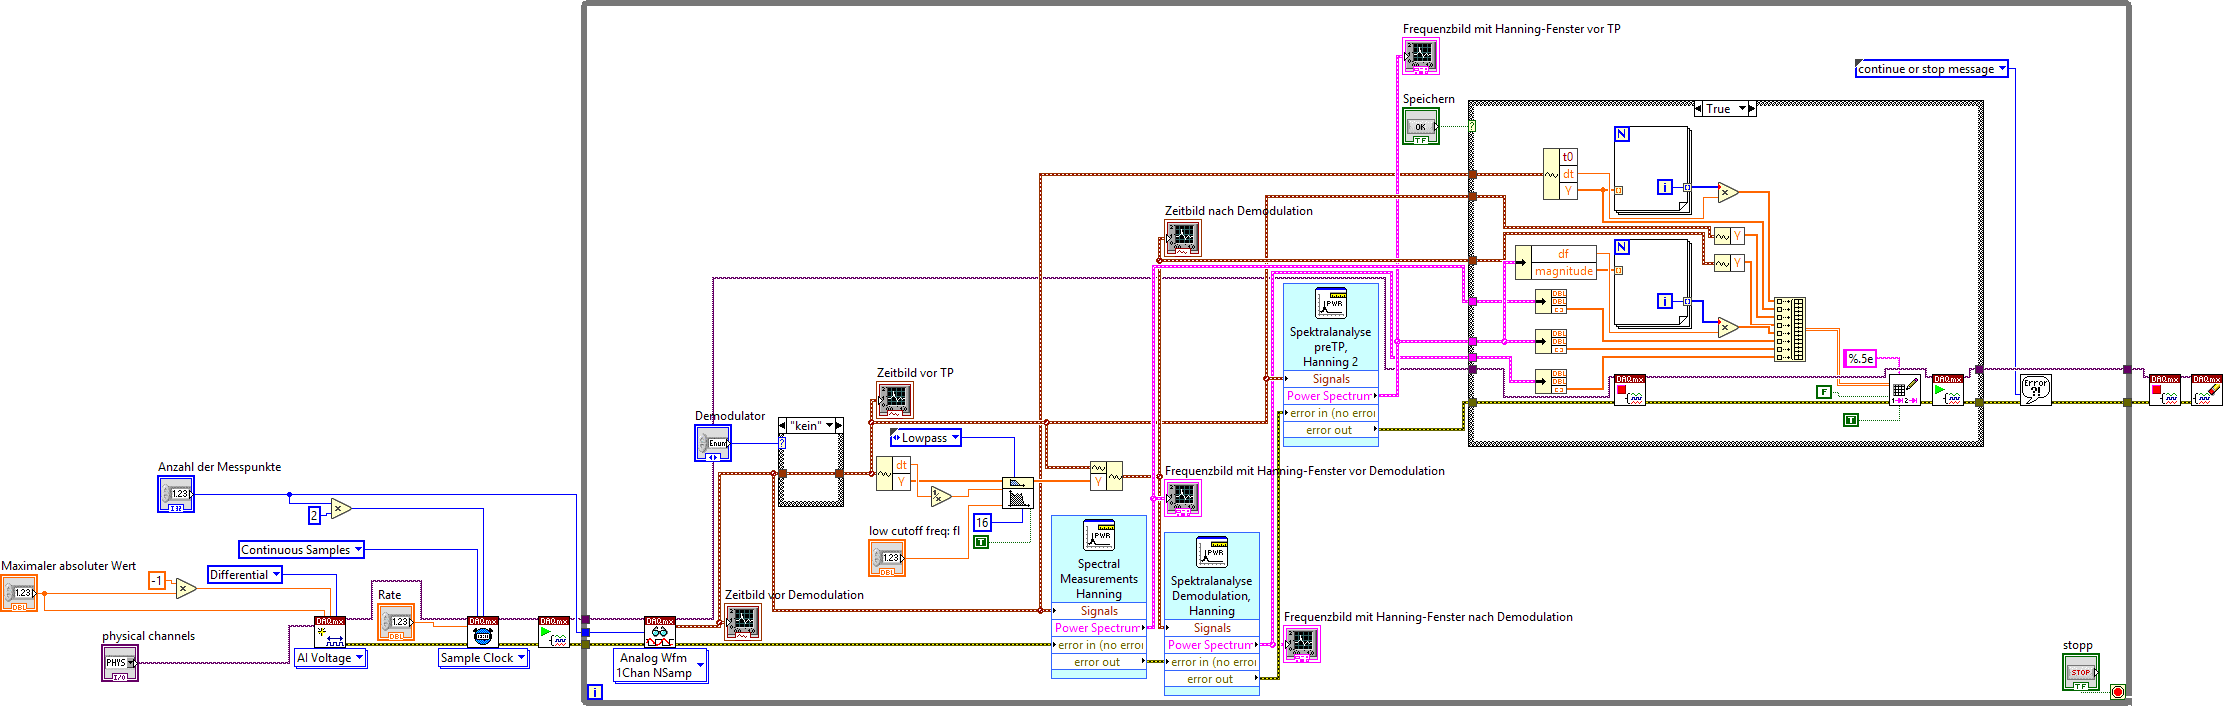
\includegraphics[width=1\textwidth]{EIRE2018Dateien/Tag3/modifizierterOszi/Oszilloskop__modifiziertd}
		\centering
		\caption{
			Blockdiagramm des Programms zur Demodulation und Darstellung eines amplitudenmodulierten Signals.
		}
		\label{fig_tag3_am_demod_block}
		\centering
	\end{figure}

	\begin{figure}[H]  
		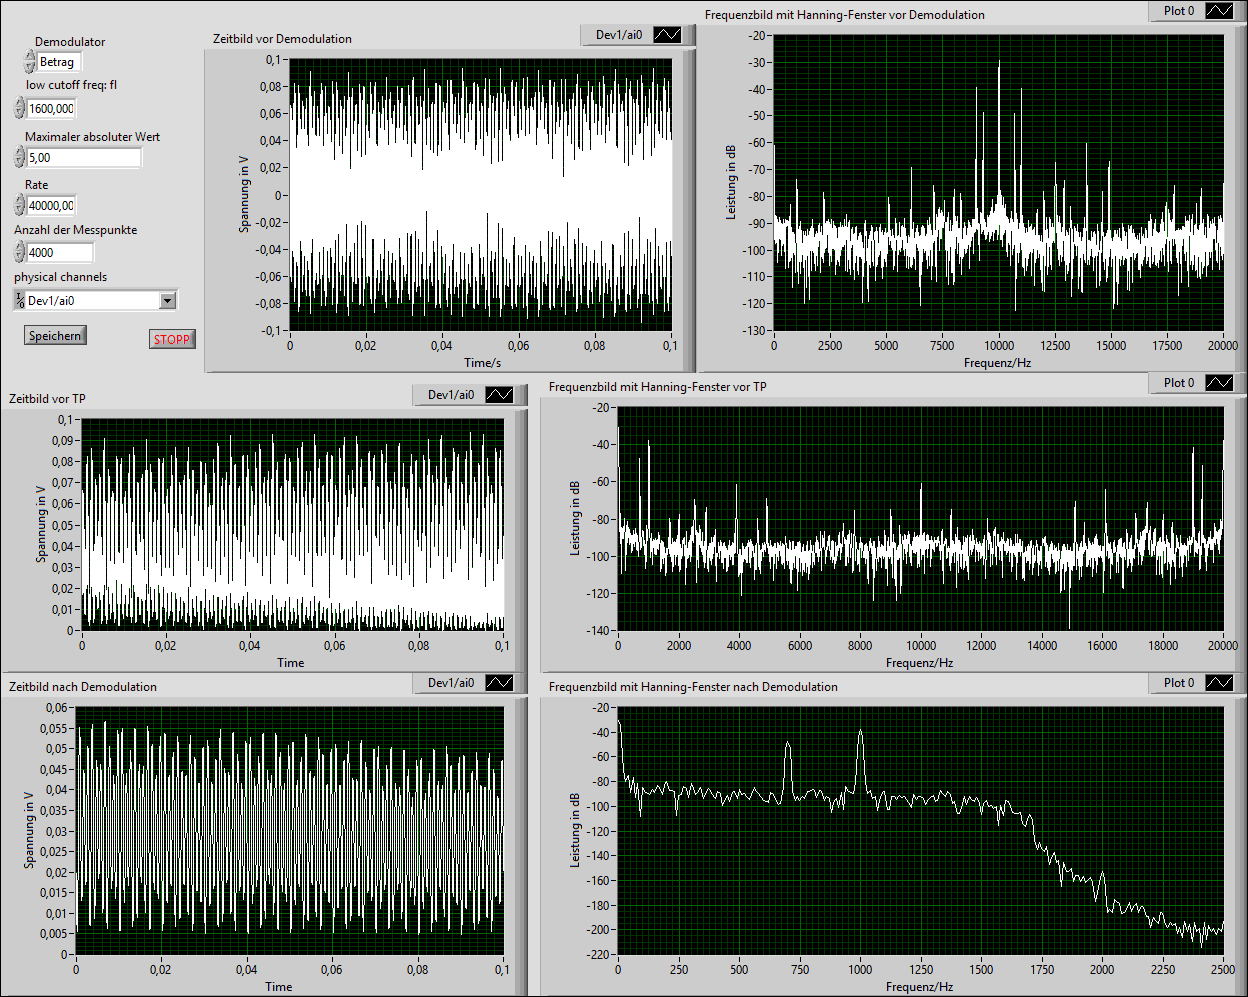
\includegraphics[width=0.7\textwidth]{EIRE2018Dateien/Tag3/modifizierterOszi/Oszilloskop__modifiziertp}
		\centering
		\caption{
			Frontplatte des Programms zur Demodulation und Darstellung eines amplitudenmodulierten Signals.
			Einstellbar ist die Art der Demodulation (keine, Quadrieren, Betragsbildung), die Grenzfrequenz des Tiefpasses nach der Demodulation, maximal messbarer Wert, Messfrequenz, Anzahl der Messpunkte pro Messdurchgang und Eingangskanal, an dem der Analog-Digital-Wandler angeschlossen ist.
			Die Grafiken zeigen jeweils im Zeit- und Frequenzbild (mit Hanning-Fensterfunktion) das Signal vor, nach und während der Demodulation.
			Die aktuellen Punkte in allen sechs Grafiken können in einer Textdatei gespeichert werden.
		}
		\label{fig_tag3_am_demod_front}
		\centering
	\end{figure}

	In \crefrange{fig_tag3_am_demod_eingang}{fig_tag3_am_demod_quadrat_vollst} sind die Graphen, die sich aus der durch den \enquote{Speichern}-Knopf erstellten Textdatei ergeben, dargestellt.
	All diesen ist gemein, dass neben den rechnerisch durch die Modulation entstehenden Frequenzen noch einige andere von signifikanter Stärke vorhanden sind.
	Diese müssen auf Störeffekte durch Netzfrequenz, deren Oberfrequenzen und andere Effekte bei der Erzeugung durch die Soundkarte zurückgeführt werden. %hab ich das nicht schon irgendwo geschrieben?
	Im Folgenden wird immer ein amplitudenmoduliertes Signal mit einer Trägerfrequenz von \SI{10000}{\hertz} verwendet.
	Vor der Modulation beinhaltet das Signal die Frequenz \SI{700}{\hertz} mit einer relativen Amplitude von \num{1} und die Frequenz \SI{1000}{\hertz} mit einer relativen Amplitude von \num{3}.
	Als Modulationsgrad wird \num{0,2} gewählt.

	\begin{figure}[H]  
		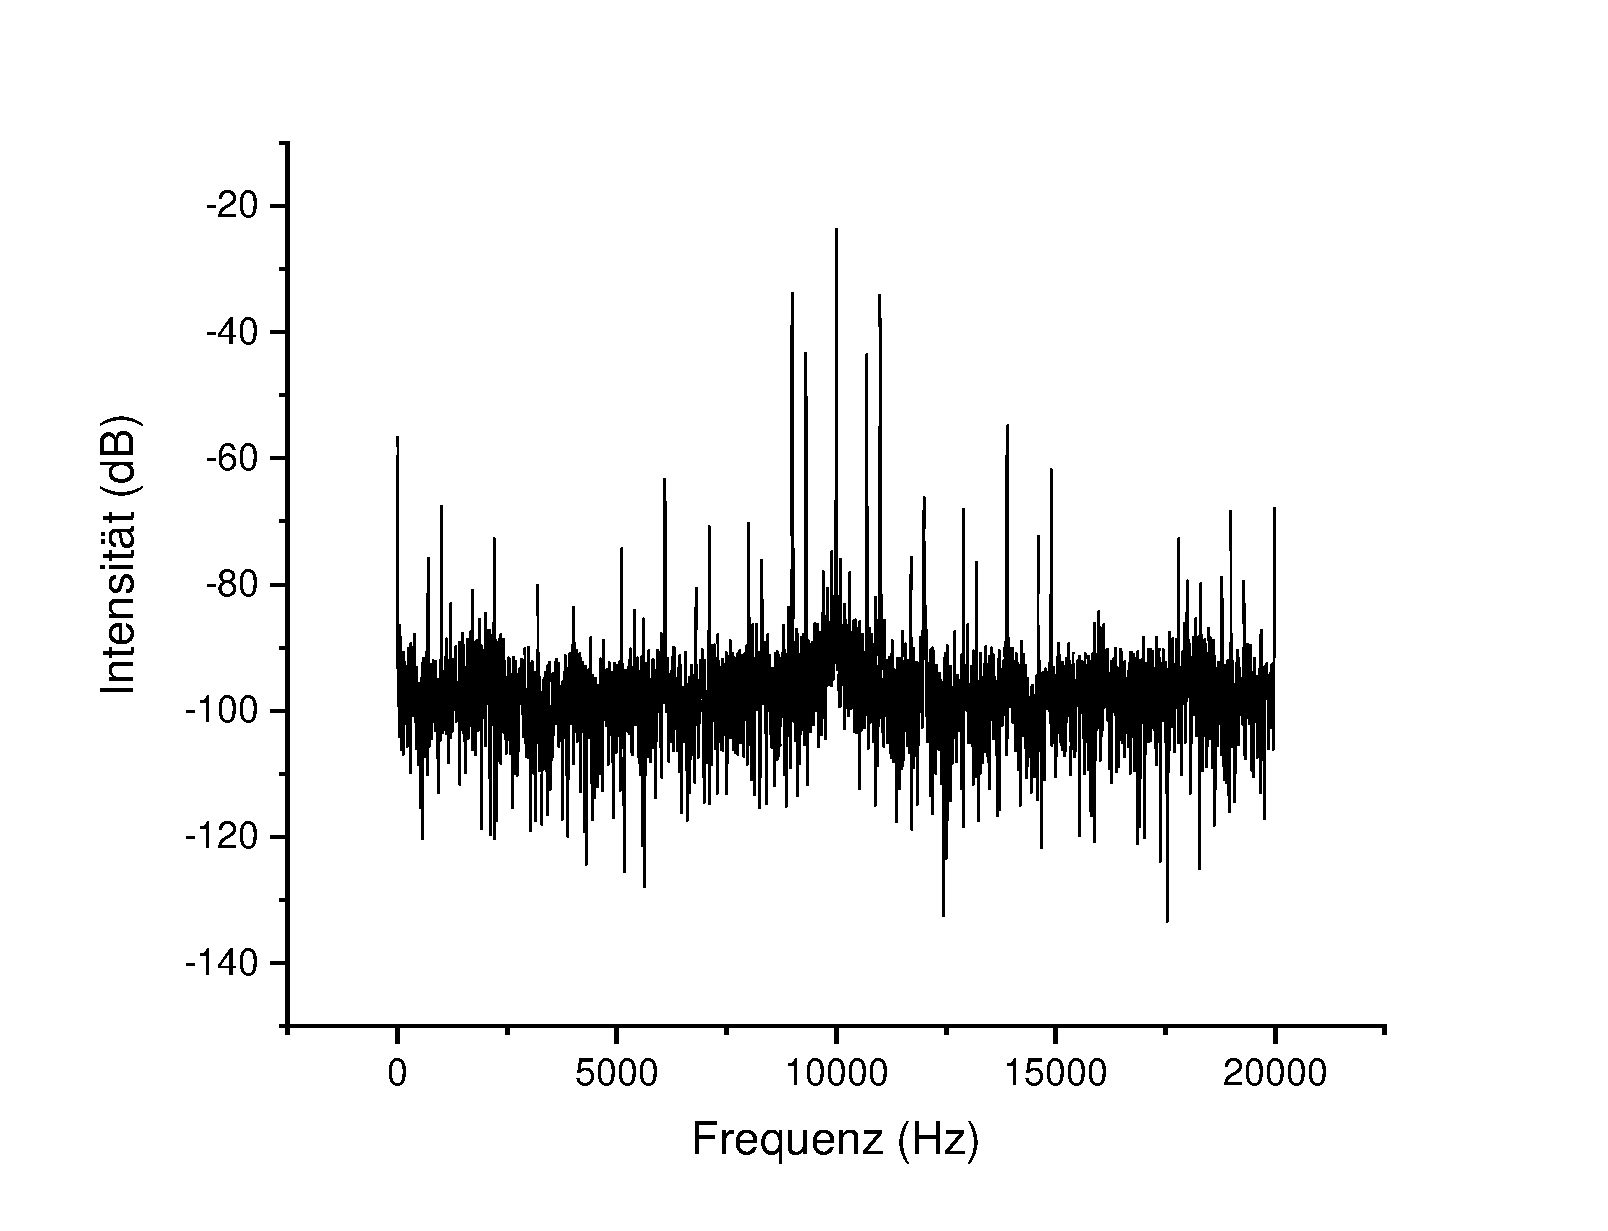
\includegraphics[width=0.7\textwidth]{Origin-Files/AM-Demod-Betrag-Eingang}
		\centering
		\caption{Ausgabe des Oszilloskopprogramms für das Eingangssignal in der Frequenzdomäne bei Eingabe eines amplitudenmodulierten Signals.
		Hierbei fällt auf, dass die Leistung des Trägersignals bei \SI{10000}{\hertz} am stärksten ist. Außerdem sind Summen- und Differenzenfrequenzen des Trägersignals mit den beiden Signalfrequenzen unmittelbar daneben bei \SI{9000}{\hertz}, \SI{9300}{\hertz}, \SI{10700}{\hertz} und \SI{11000}{\hertz} zu sehen.
		}
		\label{fig_tag3_am_demod_eingang}
		\centering
	\end{figure}

	\begin{figure}[H]  
		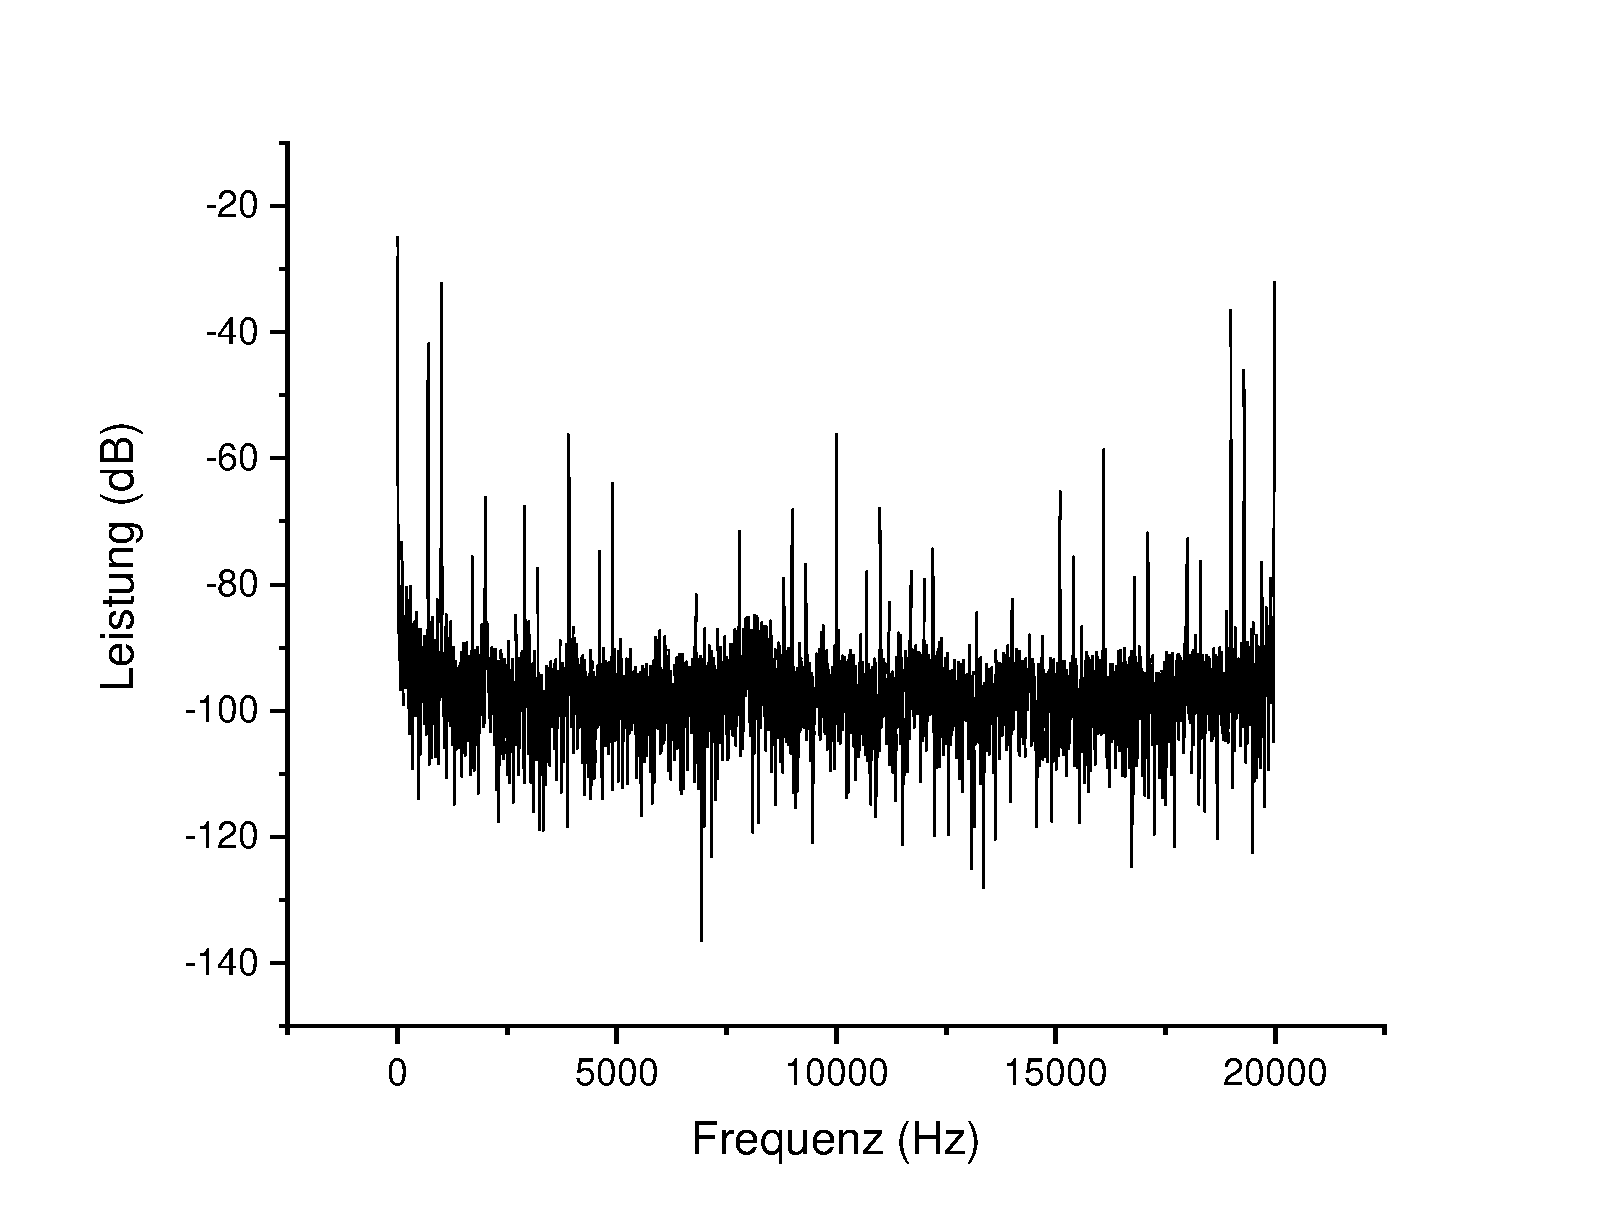
\includegraphics[width=0.7\textwidth]{Origin-Files/AM-Demod-Betrag-preTP}
		\centering
		\caption{Ausgabe des Oszilloskopprogramms in der Frequenzdomäne nach Bilden des Betrags eines amplitudenmodulierten Signals. Die Tiefpassfilterung wurde noch nicht durchgeführt.
		Dass hierin bei \SI{700}{\hertz} und \SI{1000}{\hertz} bereits die Signalfrequenzen vorhanden sind, kann nur festgestellt werden, wenn bereits bekannt ist, wo diese liegen.
		}
		\label{fig_tag3_am_demod_betrag_preTP}
		\centering
	\end{figure}

	\begin{figure}[H]
		\centering
		\begin{subfigure}[t]{0.5\textwidth}
			\centering
			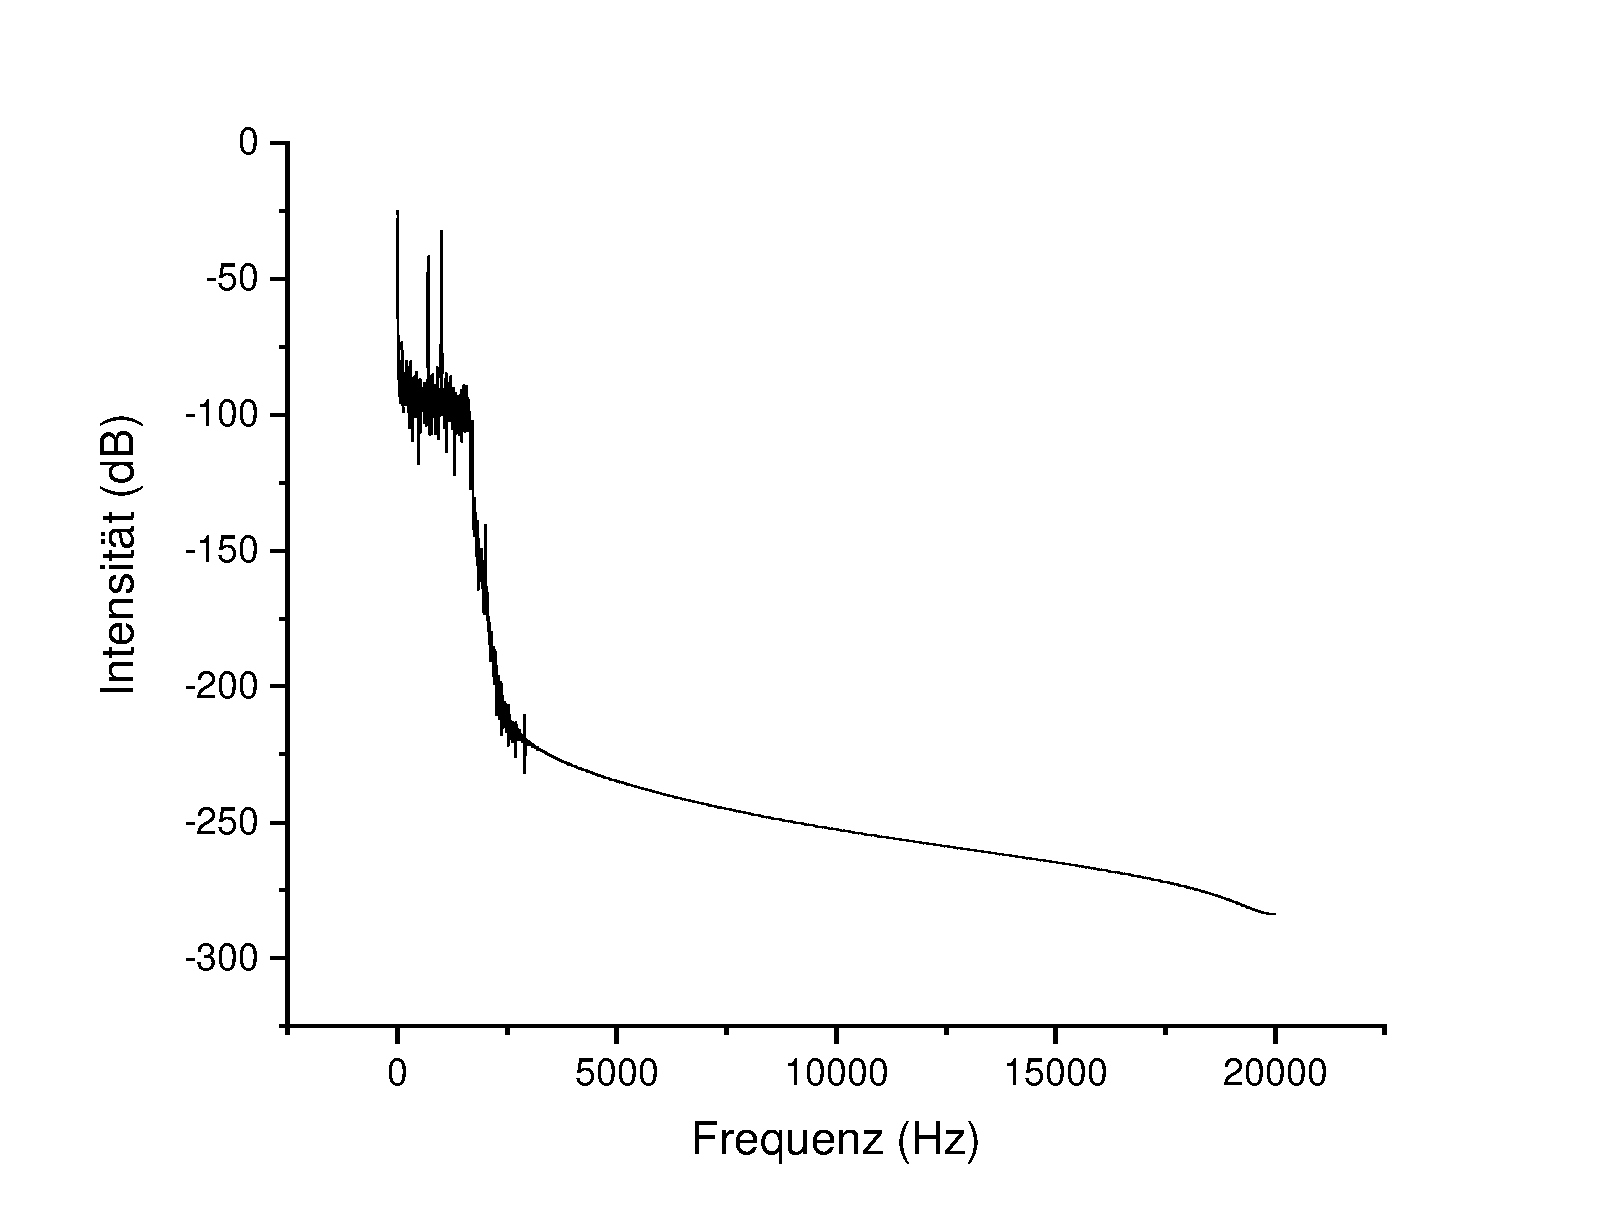
\includegraphics[width=1\textwidth]{Origin-Files/AM-Demod-Betrag-demod}
			\caption{gesamter Frequenzbereich}
		\end{subfigure}%
		\begin{subfigure}[t]{0.5\textwidth}
			\centering
			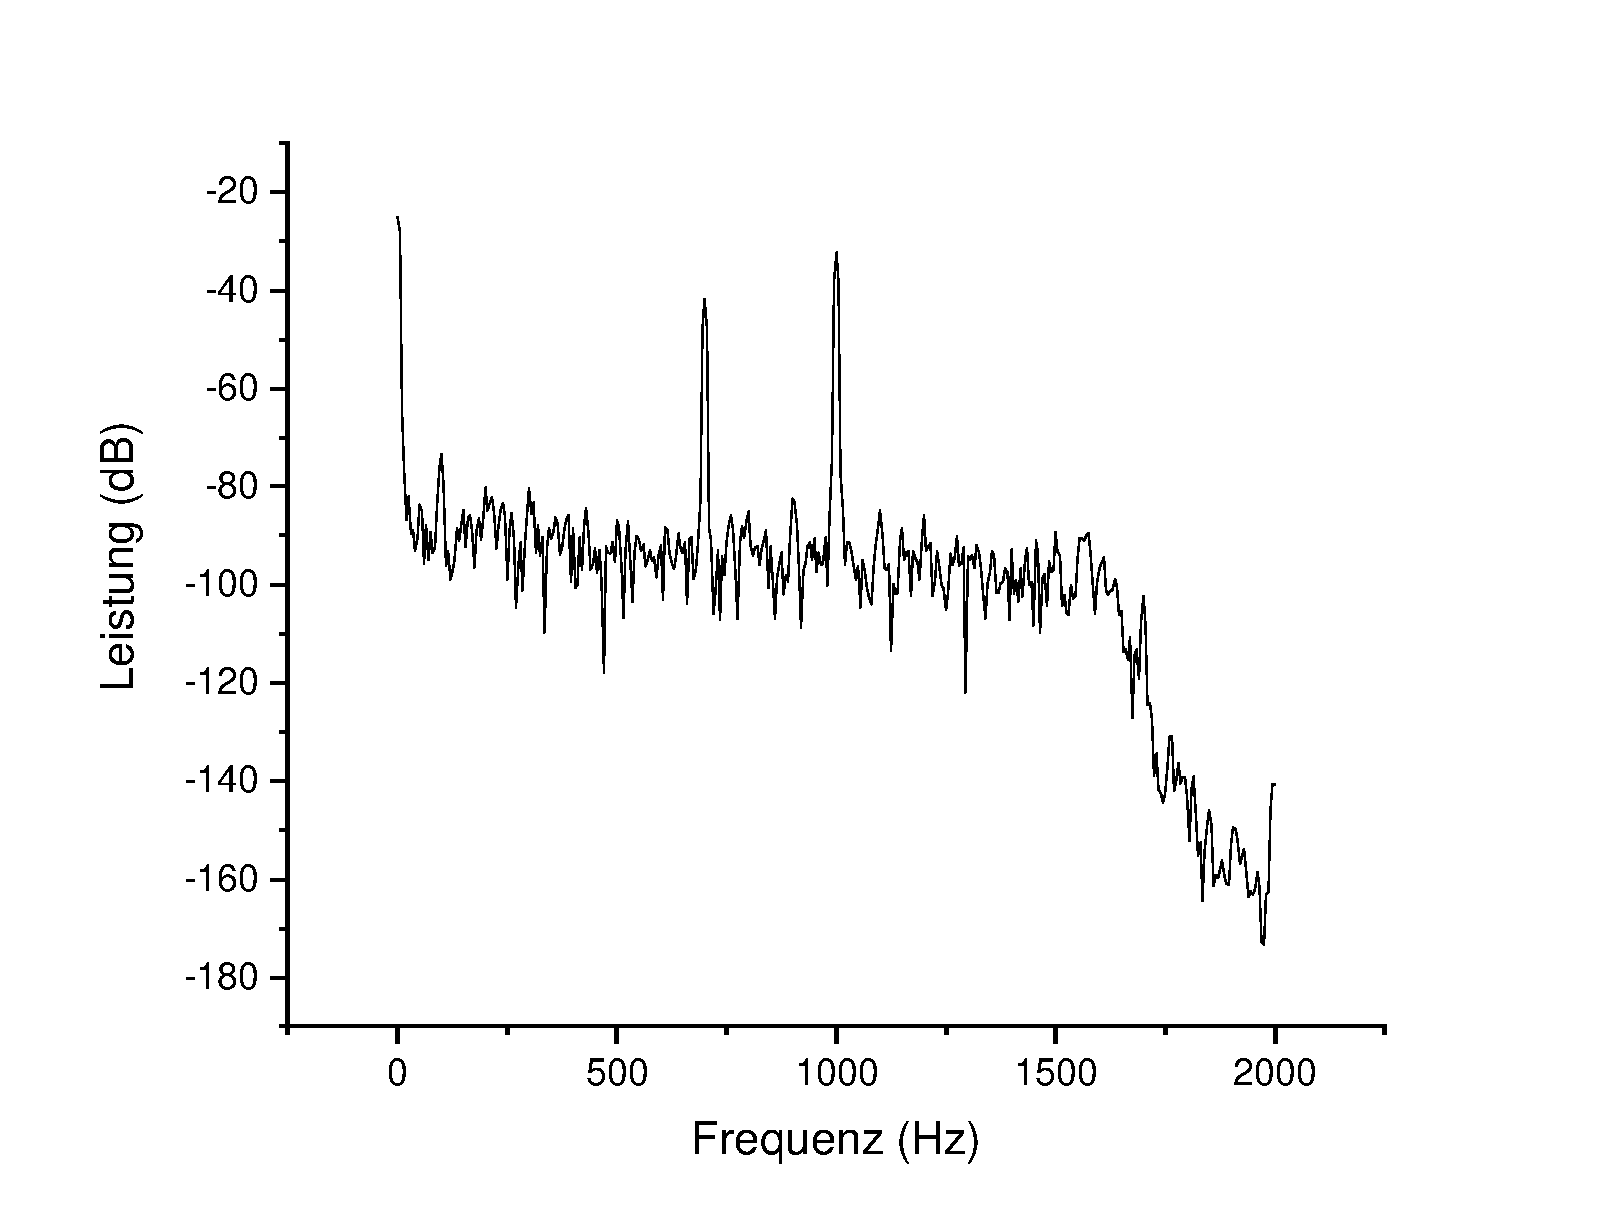
\includegraphics[width=1\textwidth]{Origin-Files/AM-Demod-Betrag-demod-Bereich}
			\caption{geringer Frequenzbereich}
		\end{subfigure}
		\label{fig_tag3_am_demod_betrag_vollst}
		\caption{Ausgabe des Oszilloskopprogramms in der Frequenzdomäne nach vollständiger Demodulation durch Bilden des Betrags und Tiefpassfilterung des amplitudenmodulierten Signals.
		Als Grenzfrequenz für den Tiefpass wurde \SI{1600}{\hertz} gewählt.
		Hierfür muss man voraussetzen, dass bekannt ist, in welchem Frequenzbereich sich die Frequenzen im Signal befinden.
		In der Darstellung des Frequenzbereichs von \SIrange{0}{2000}{\hertz} sind beide Signalfrequenzen sowie ein signifikanter Gleichanteil zu erkennen. %ja den könnte man mit Hochpass wegmachen, muss man das erwähnen? denke nicht
		}
		\centering
	\end{figure}



\iffalse %auskommentiert, weil natürlich gleich wie Betrag
	\begin{figure}[H]  
		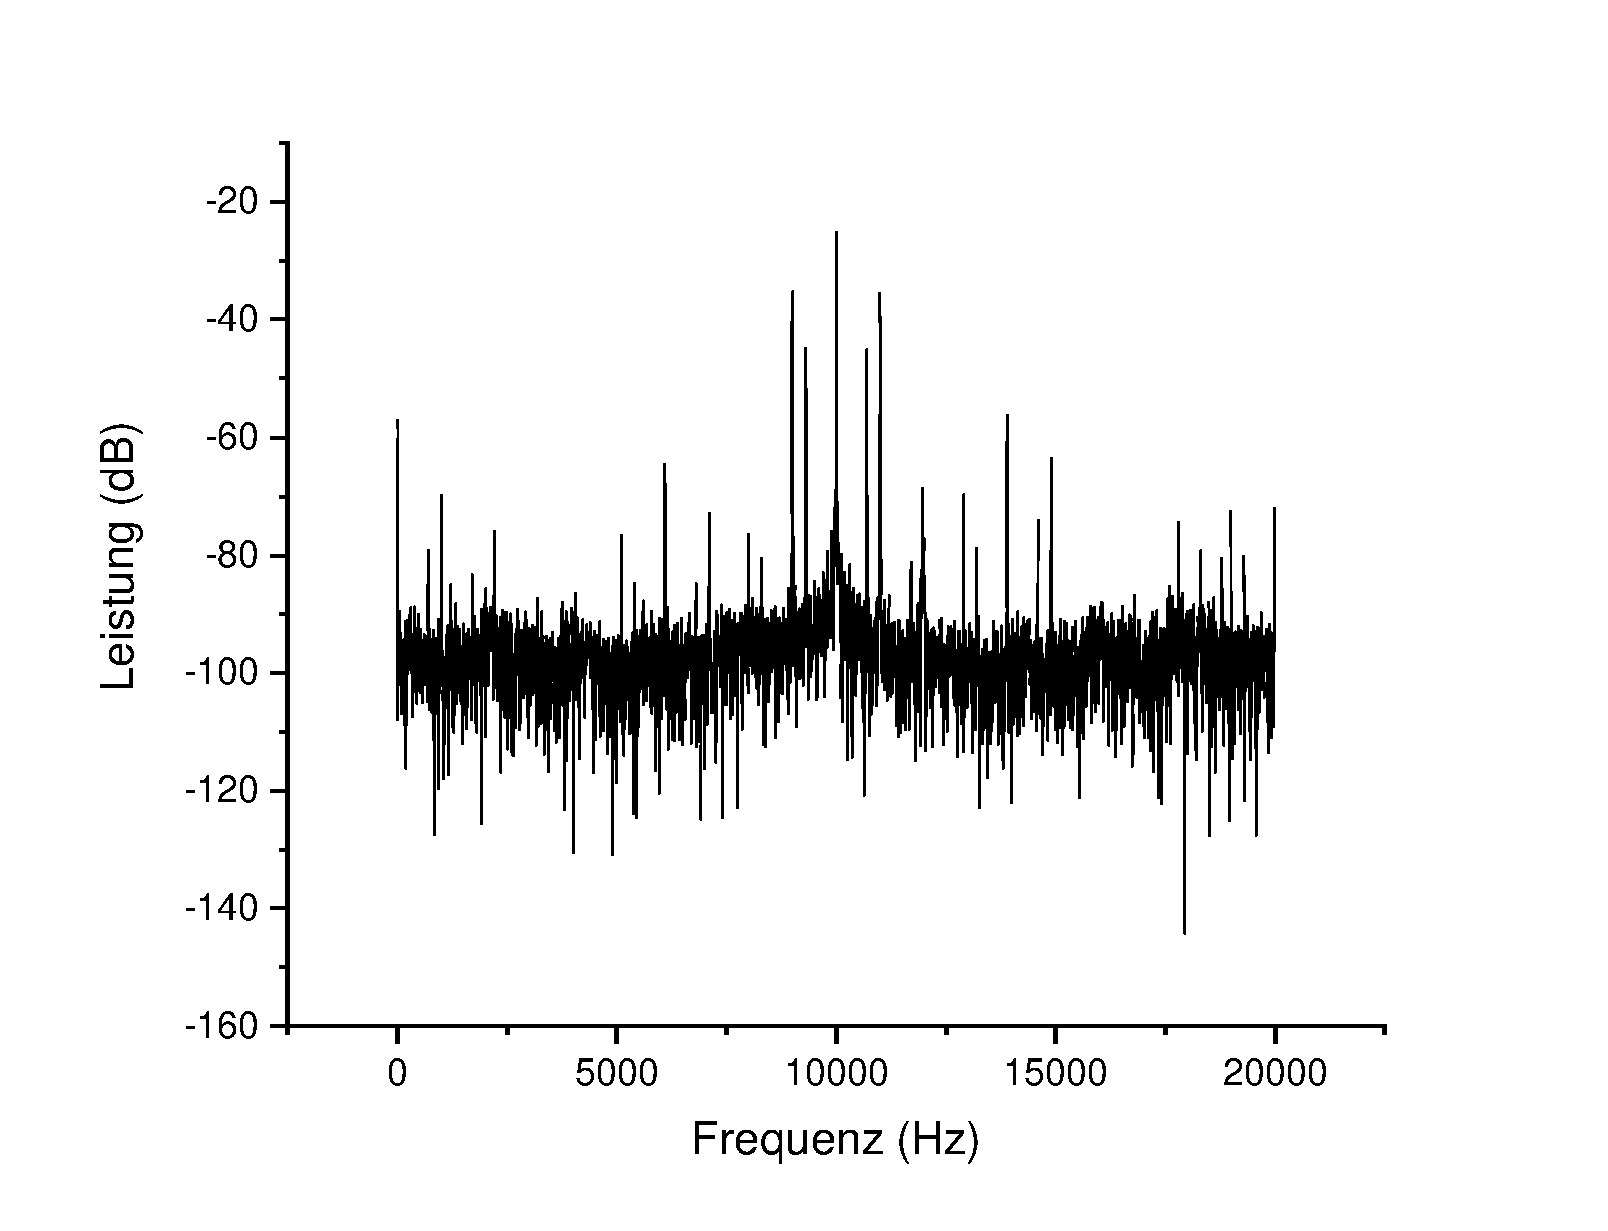
\includegraphics[width=0.7\textwidth]{Origin-Files/AM-Demod-Quadrat-Eingang}
		\centering
		\caption{abc
		}
		\label{}
		\centering
	\end{figure}
\fi

	\begin{figure}[H]  
		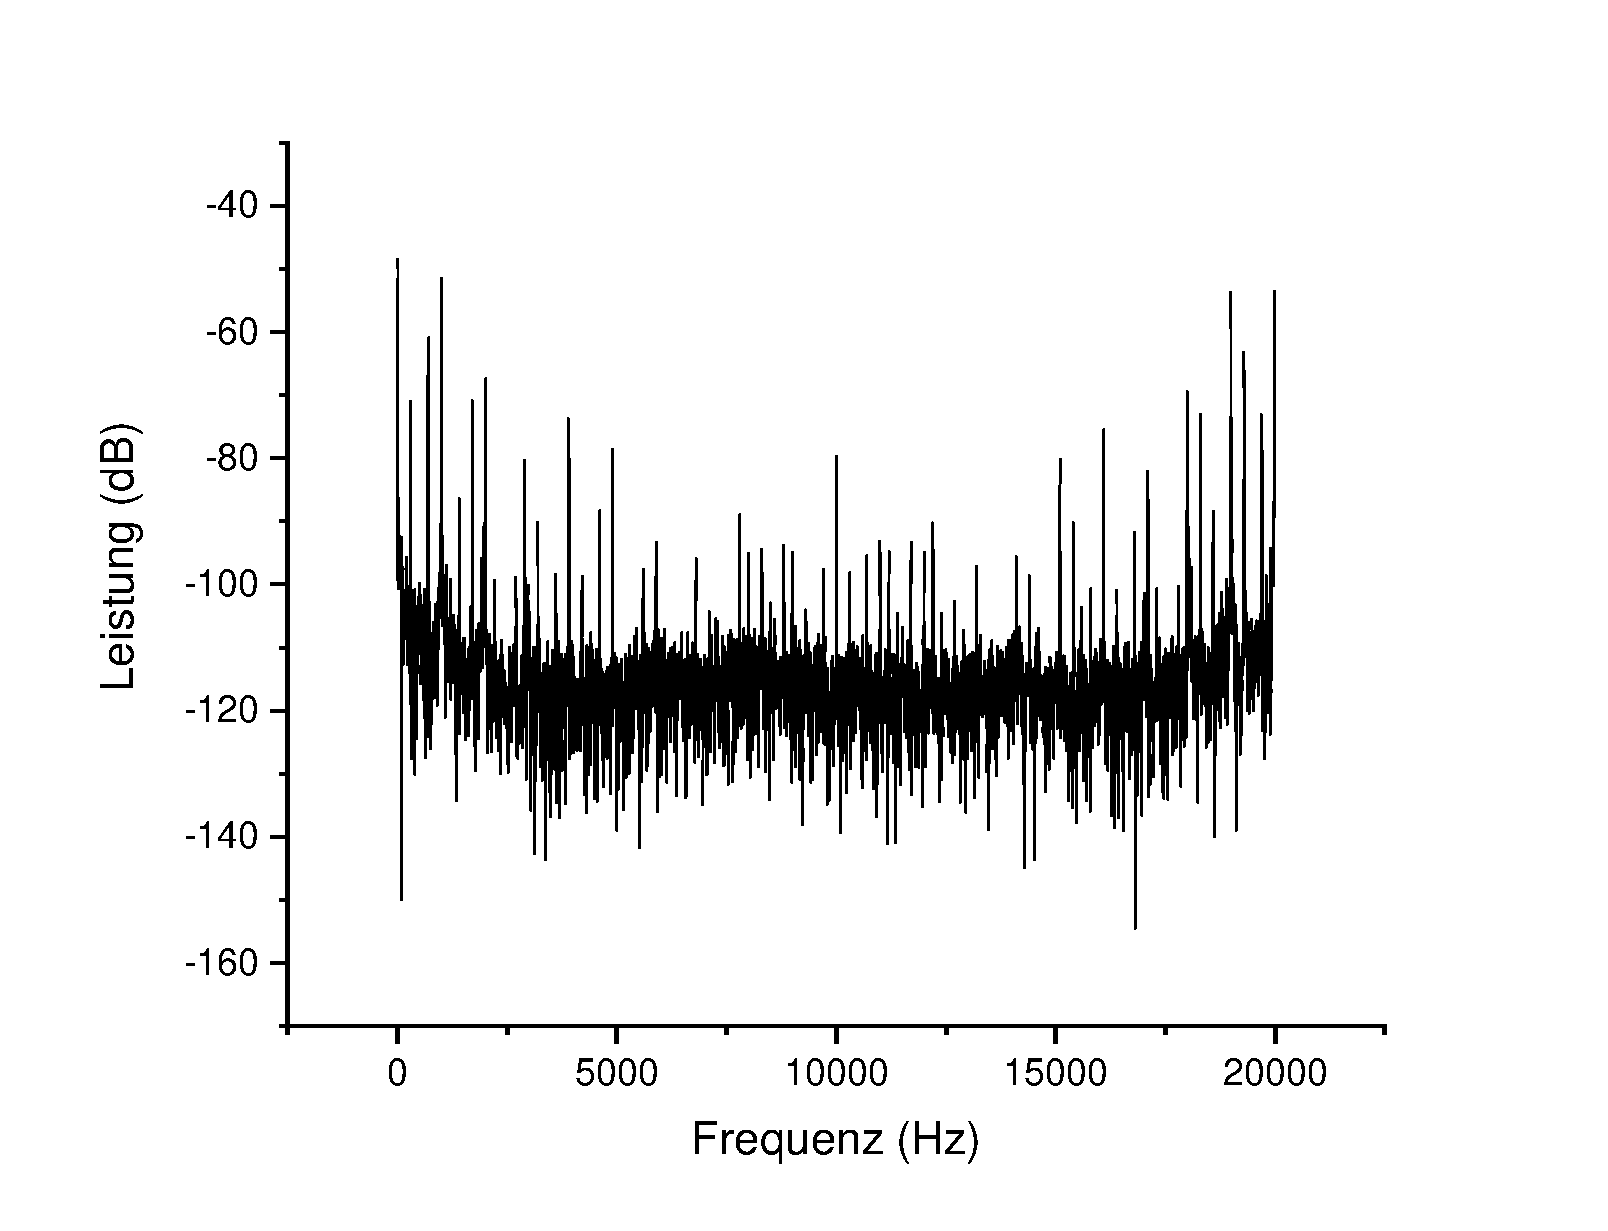
\includegraphics[width=0.7\textwidth]{Origin-Files/AM-Demod-Quadrat-preTP}
		\centering
		\caption{Ausgabe des Oszilloskopprogramms in der Frequenzdomäne nach Quadrieren eines amplitudenmodulierten Signals. Die Tiefpassfilterung wurde noch nicht durchgeführt.
		Dass hierin bei \SI{700}{\hertz} und \SI{1000}{\hertz} bereits die Signalfrequenzen vorhanden sind, kann nur festgestellt werden, wenn bereits bekannt ist, wo diese liegen.
		}
		\label{fig_tag3_am_demod_quadrat_preTP}
		\centering
	\end{figure}

	\begin{figure}[H]
		\centering
		\begin{subfigure}[t]{0.5\textwidth}
			\centering
			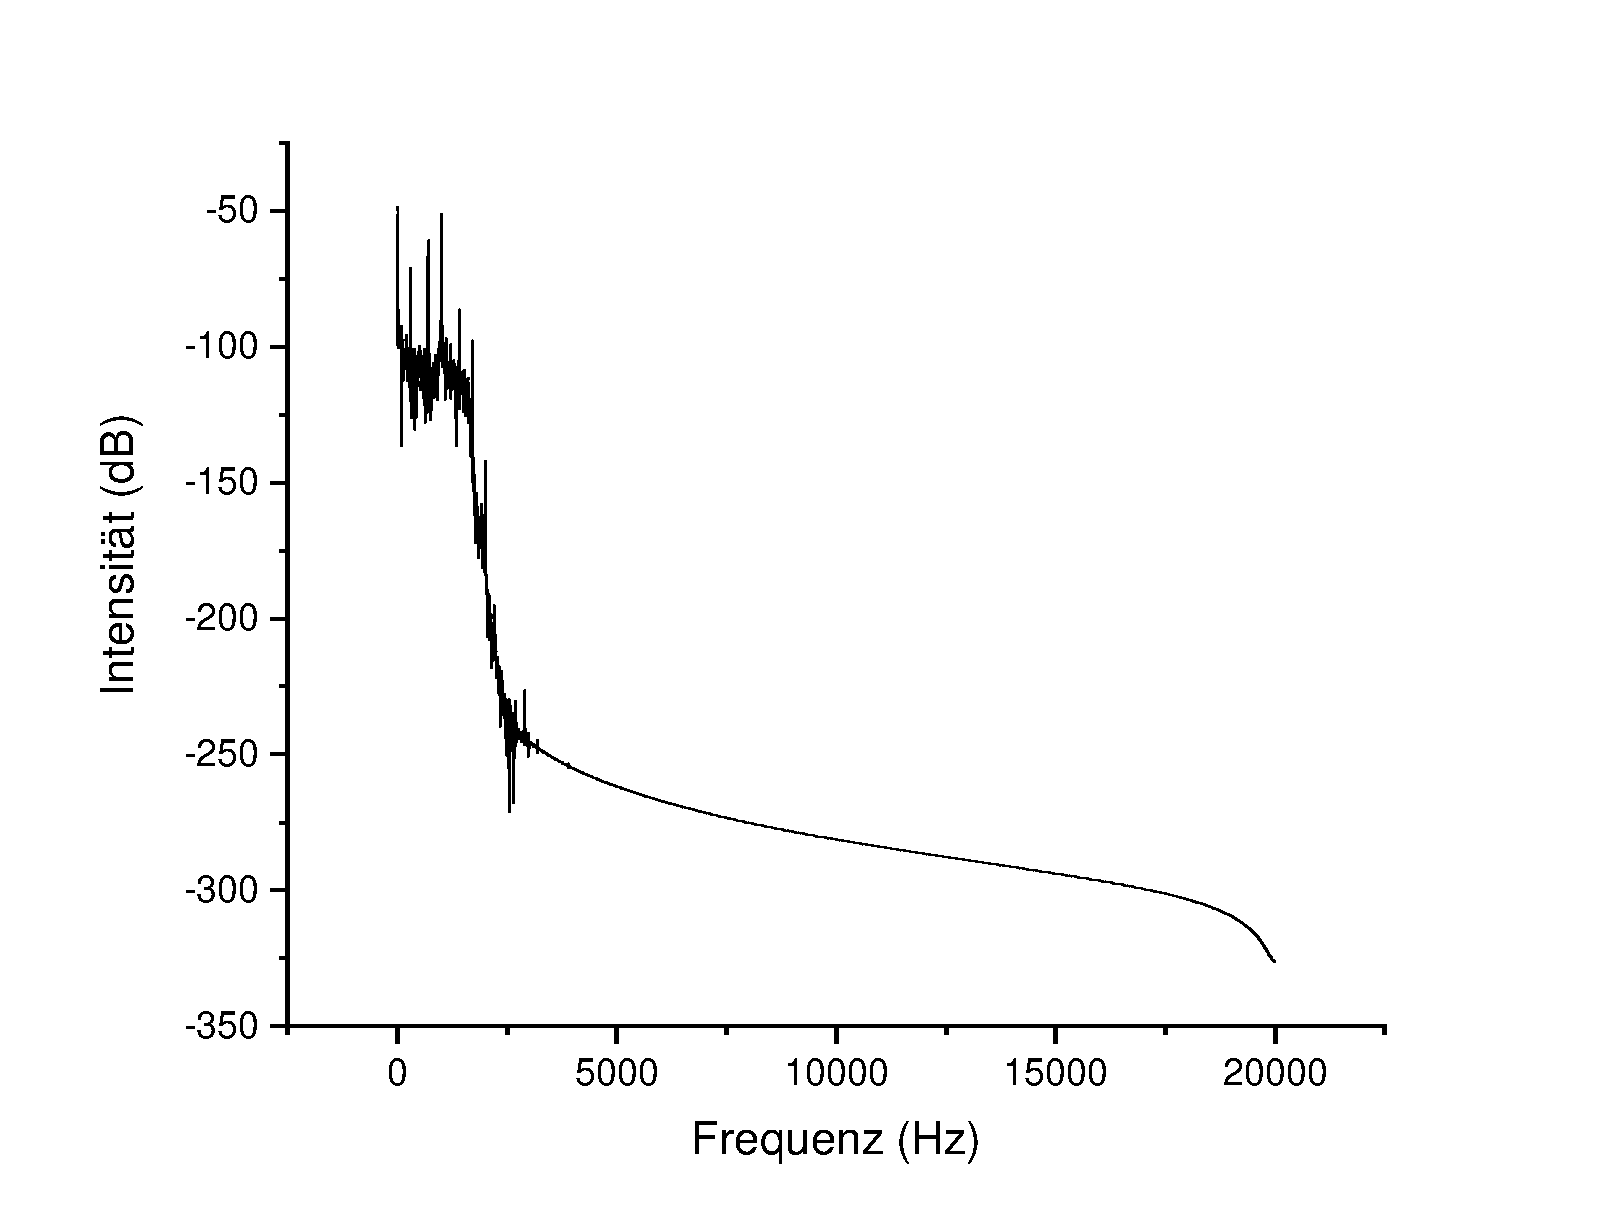
\includegraphics[width=1\textwidth]{Origin-Files/AM-Demod-Quadrat-demod}
			\caption{gesamter Frequenzbereich}
		\end{subfigure}%
		\begin{subfigure}[t]{0.5\textwidth}
			\centering
			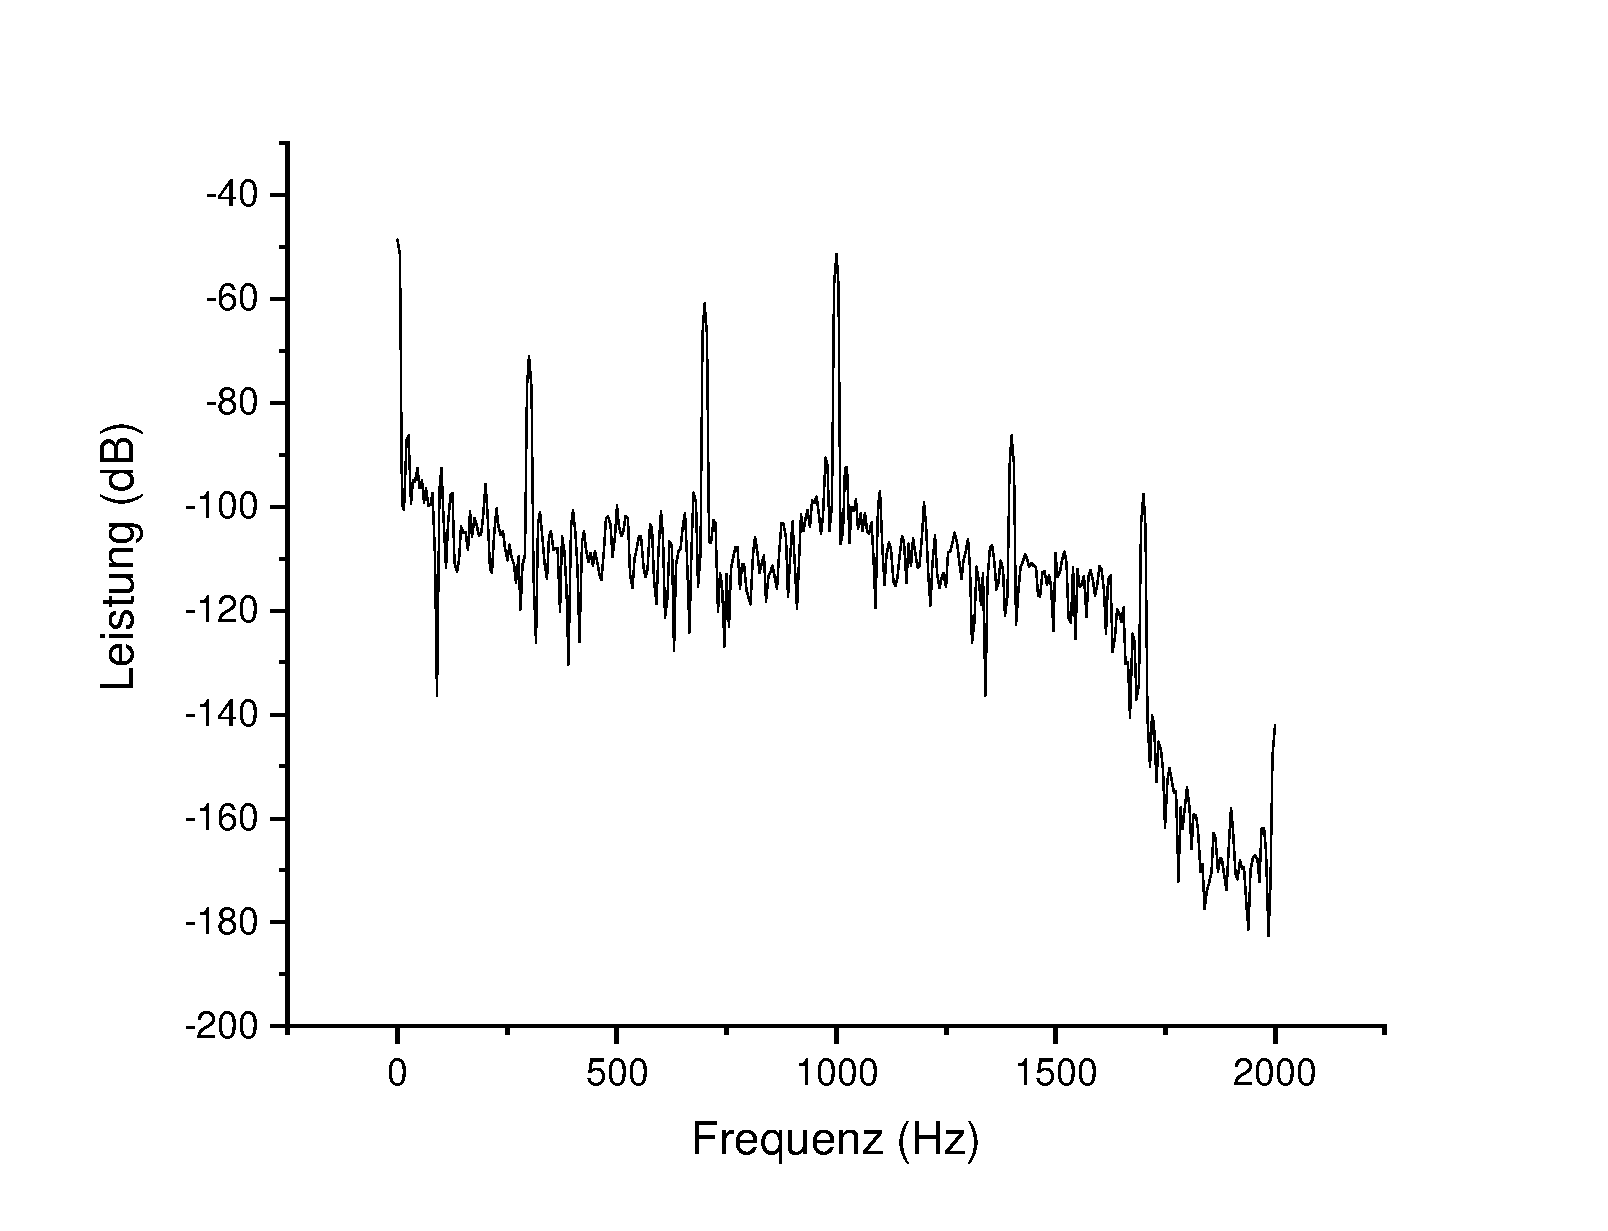
\includegraphics[width=1\textwidth]{Origin-Files/AM-Demod-Quadrat-demod-Bereich}
			\caption{geringer Frequenzbereich}
			\label{fig_tag3_am_demod_quadrat_vollst}
		\end{subfigure}
	
		\caption{Ausgabe des Oszilloskopprogramms in der Frequenzdomäne nach vollständiger Demodulation durch Quadrieren und Tiefpassfilterung des amplitudenmodulierten Signals.
		Als Grenzfrequenz für den Tiefpass wurde \SI{1600}{\hertz} gewählt.
		Hierfür muss man voraussetzen, dass bekannt ist, in welchem Frequenzbereich sich die Frequenzen im Signal befinden.
		In der Darstellung des Frequenzbereichs von \SIrange{0}{2000}{\hertz} sind beide Signalfrequenzen sowie ein signifikanter Gleichanteil zu erkennen.
		Hier treten allerdings noch einige zusätzliche Frequenzen auf, weshalb die Bildung des Betrages gegenüber dem Quadrieren zu bevorzugen ist.
		}
		\centering
	\end{figure}

	%TODO Ist das ok, wenn hier alle Erkenntnisse in den Captions stehen?


	
	\subsection{Demodulation eines AM-Signals mittels Trägerfrequenzmultiplikation} \label{DemodTraeger}
	
	Das allgemeine Ziel dieses Abschnitts ist die Demodulation eines über den Analog-Digital-Wandler in Verbindung mit der Computer-Soundkarte gemessenen amplitudenmodulierten Signals unter Zuhilfenahme der Multiplikation mit der Trägerfrequenz. 
	In der mathematischen Theorie führt das Multiplizieren der amplitudenmodulierten Signal-Funktion mit der Schwingungsfunktion, welche lediglich der Trägerfrequenz des AM-Signals unterliegt, dazu, dass sich mit dem passenden Additionstheorem als Ergebnis eine additive Aneinanderreihung von Schwingungstermen unterschiedlichster Frequenzen bildet. 
	Letztere lassen sich unter Verwendung einer Fourier-Transformation im Frequenzspektrum dieses neu gewonnenen Schwingungsterms betrachten. 
	Neben den diversen Peaks an Stellen mit vergleichsweise hohen Frequenzen, befinden sich darin ebenfalls Peaks bei relativ niedrigen Frequenzwerten.
		
	\begin{figure}[H]
		\centering
		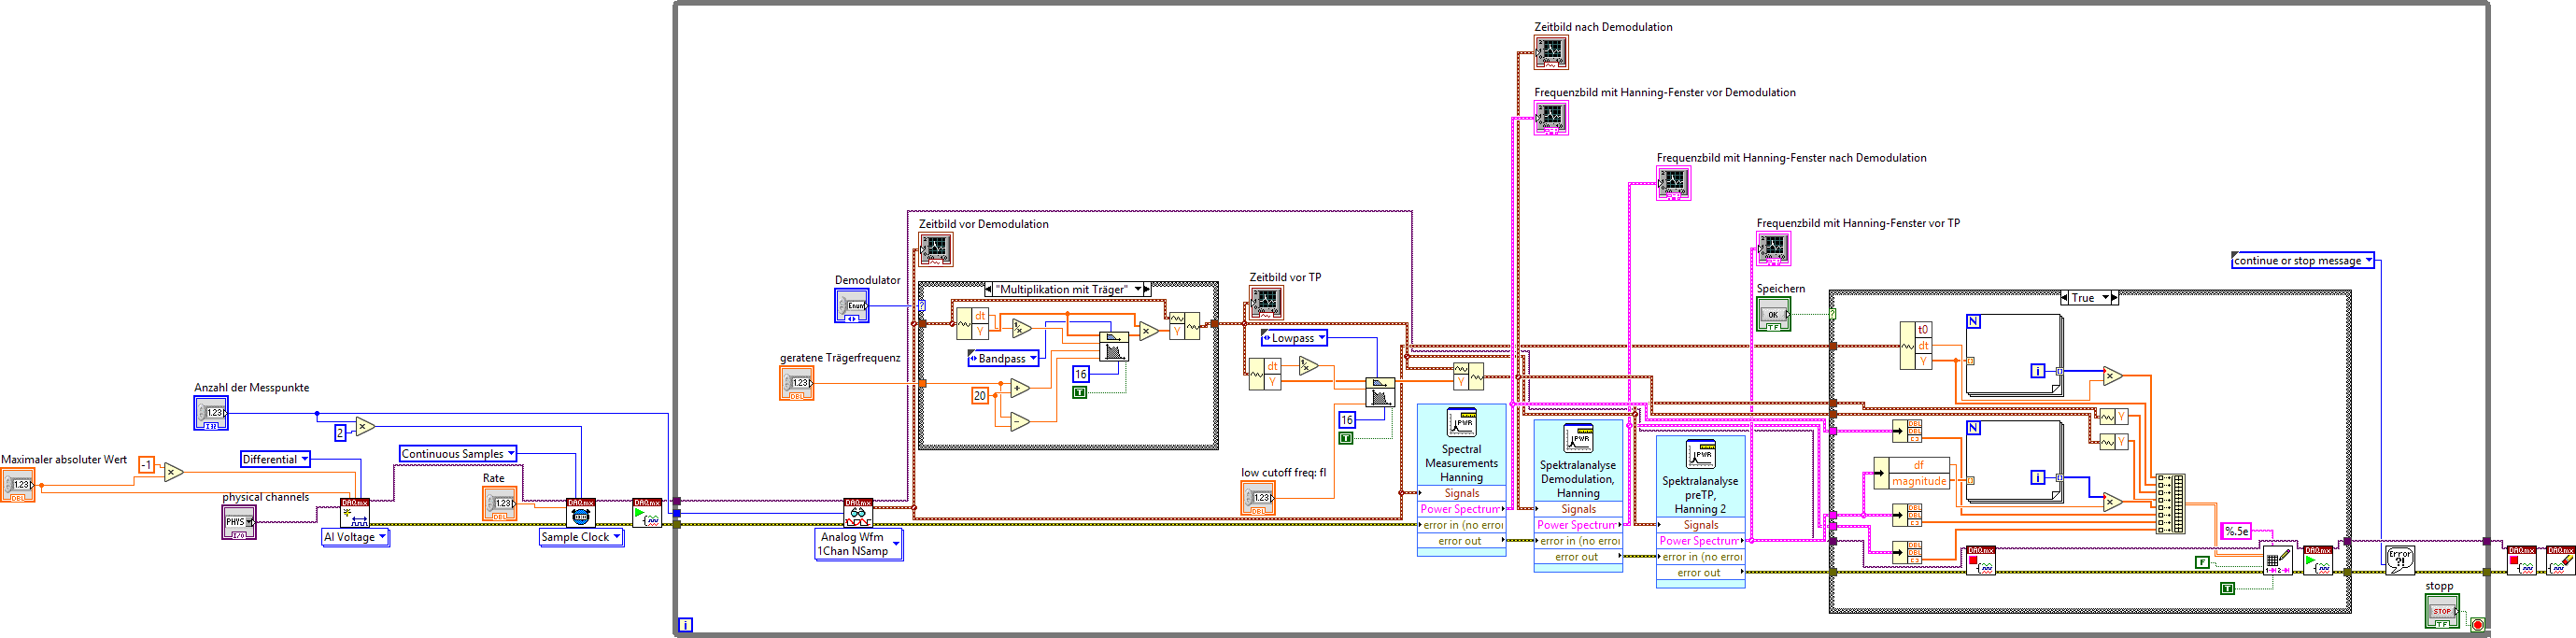
\includegraphics[width=1.0\textwidth]{EIRE2018Dateien/Tag4/traegerMultOszi/Oszilloskop__modifiziertd}
		\caption{Die Abbildung zeigt das LabVIEW-Blockdiagramm bzw. den Programmcode zur Demodulation eines über den Analog-Digital-Wandler in Kombination mit der Computer-Soundkarte gemessenen amplitudenmodulierten Signals mittels Trägerfrequenzmultiplikation.}
		\label{MultiTraegerProgrammcode}
	\end{figure}

	\noindent Demnach handelt es sich um ein breites Frequenzspektrum, in dem man sogar die Frequenz(en) des modulierten, ursprünglichen Signals deutlich erkennen kann. 
	Von einem theoretischen Standpunkt aus ist die komplette Demodulation des AM-Signals damit abgeschlossen. 
	Zusätzlich lassen sich durch einen Tiefpass mit hinreichend großer Grenzfrequenz die hohen Frequenzanteile aus dem Spektrum herausfiltern, sodass letztendlich nur noch die besagten Frequenzen des amplitudenmodulierten Ursprungssignals übrig bleiben. 
	
	Dieses Verfahren soll nun in ein LabVIEW-Programm übertragen werden, dessen dazugehöriger Programmcode in \ref{MultiTraegerProgrammcode} zu sehen ist. 
	Voraussetzung ist dabei das in \cref{DemodulationAM} bereits erstellte Programm.
	Alle zuvor eingefügten Methoden zur Demodulation (\glqq Quadrat\grqq\ und \glqq Betrag\grqq ) sollen frei auswählbar bleiben.
	Dafür wird zunächst die Demodulator-Case-Konstruktion um eine weitere Option mit dem Namen \glqq Multiplikation mit Träger\grqq\ ergänzt und somit ein neues, ausfüllbares Case-Feld erzeugt.
	Darin werden diverse, später näher beschriebene Blockdiagrammobjekte angelegt, welche die Demodulation des über den Analog-Digital-Wandler in Verbindung mit der Computer-Soundkarte gemessenen AM-Signals umsetzten.
	Zuerst muss hierbei vom Nutzer die Trägerfrequenz des amplitudenmodulierten Signals geraten werden.
	Dazu wird sowohl ein weiteres Bedienelement auf dem Frontpanel hinzugefügt als auch ein entsprechendes Blockdiagrammobjekt im Programmcode erstellt.
	
	\begin{figure}[H]
		\centering
		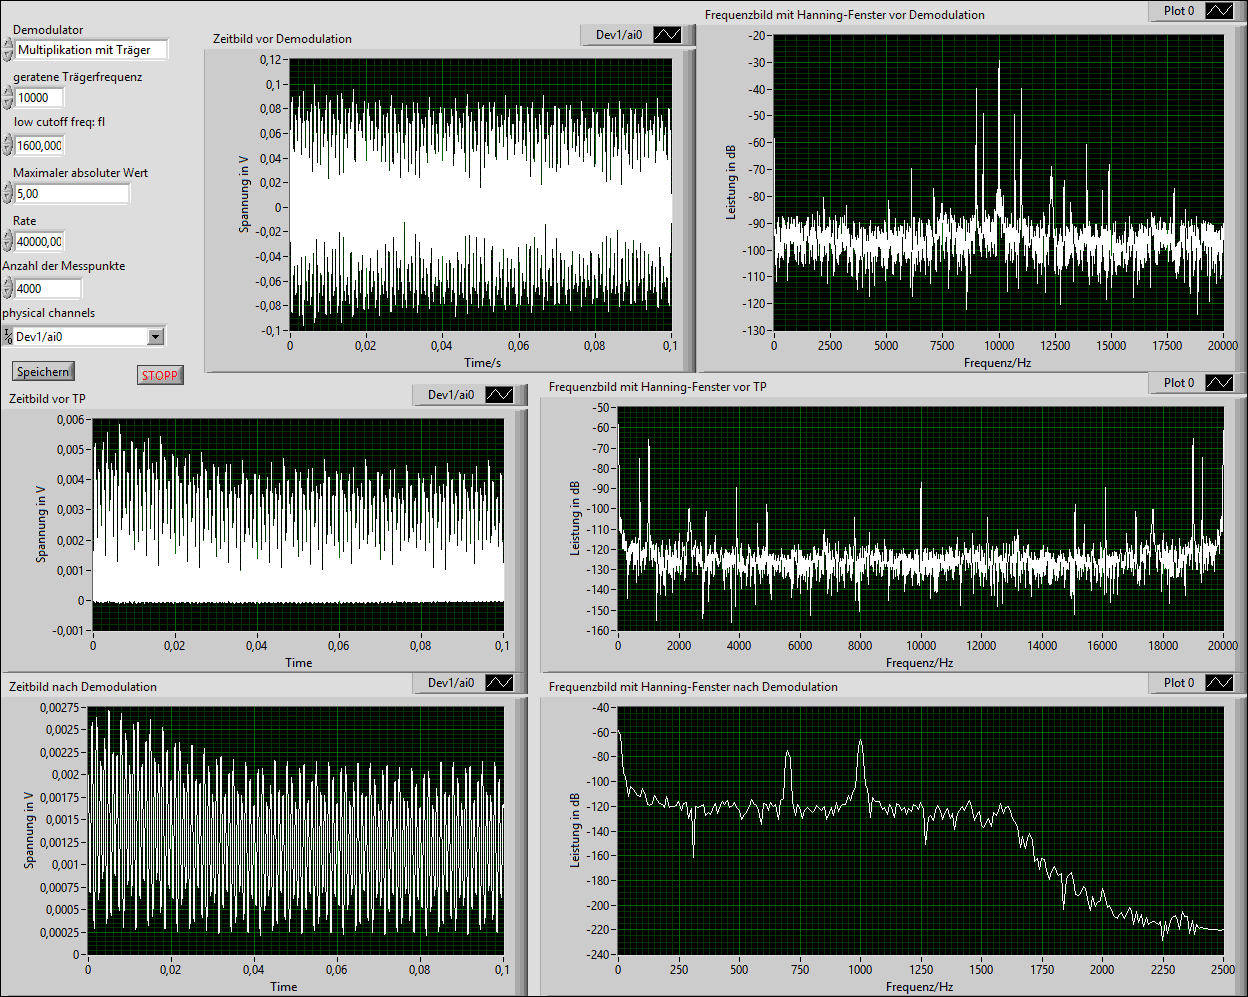
\includegraphics[width=1.0\textwidth]{EIRE2018Dateien/Tag4/traegerMultOszi/Oszilloskop__modifiziertp}
		\caption{Die Abbildung veranschaulicht die LabVIEW-Benutzeroberfläche bzw. das LabVIEW-Frontpanel des Programms zur Demodulation eines über den Analog-Digital-Wandler in Kombination mit der Computer-Soundkarte gemessenen AM-Signals mittels Trägerfrequenzmultiplikation. Alle sechs Anzeige- bzw. Ausgabeelemente zeigen in zweidimensionalen, kartesischen Diagrammen das an bestimmten Stellen des Bearbeitungsprozesses abgegriffene AM-Signal, jeweils im Zeitbild und im Frequenzbild mit Hanning-Fenster. Die beiden oberen Diagramme stellen das über den Analog-Digital-Wandler in Verbindung mit der Computer-Soundkarte gemessene AM-Signal vor der Demodulation dar. In den beiden mittleren Diagrammen sieht man das Ergebnis der Demodulation des amplitudenmodulierten Signals ohne Tiefpassfilterung. Die unteren beiden Diagramme veranschaulichen das demodulierte AM-Signal nach der Tiefpassfilterung.}
		\label{MultiTraegerFrontpanel}
	\end{figure}

	\noindent Mit einem Bandpass sechzehnter Ordnung soll die geratene Trägerfrequenz aus dem Frequenzspektrum des AM-Signals herausgefiltert werden. 
	Die obere bzw. untere Grenzfrequenz des Bandpassfilters bildet der geratene Trägerfrequenzwert zuzüglich bzw. abzüglich einem Wert von $20\,$Hz. 
	Dieser $20\,$Hz-Wert ist hinreichend groß gewählt, um einerseits Überlappungen mit anderen Frequenz-Peaks zu vermeiden und andererseits die Gesamtheit des Trägerfrequenz-Peaks zu erfassen. 
	Es wird also ein Bereich von $\pm 20\,$Hz um die Trägerfrequenz \glqq herausgeschnitten\glqq . 
	Die dazugehörige Schwingungsfunktion wird nun mit dem unveränderten, gemessenen amplitudenmodulierten Signal multipliziert. 
	Das Ergebnis dieser Operation ist, wie zuvor im Theorie-Teil erwähnt, ein breites Frequenzspektrum mit zahlreichen Peaks an unterschiedlich hohen und niedrigen Frequenzwerten, was im rechten, mittleren Diagramm in \cref{MultiTraegerFrontpanel} erkennbar ist. 
	Überdies sind in \cref{MultiTraegerFrontpanel} noch fünf weitere Anzeigeelemente in Diagramm-Form dargestellt: Die beiden Oberen zeigen das über den Analog-Digital-Wandler in Kombination mit der Computer-Soundkarte gemessene amplitudenmodulierte Signal ohne Demodulation, zum einen im Zeitbild und zum andern im Frequenzbild. 
	Im linken, mittleren Anzeigeelement ist ein Diagramm zu sehen, in dem der zeitliche Signalverlauf nach der Durchführung der Trägerfrequenzmultiplikation und somit auch nach der kompletten Demodulation veranschaulicht ist. 
	Die beiden unteren Anzeigeelemente stellen, sowohl im Zeit- als auch im Frequenzbild, das demodulierte AM-Signal nach der bereits im Theorie-Teil angesprochenen Tiefpassfilterung dar. 
	Genauso wie in \cref{DemodulationAM} findet die Tiefpassfilterung außerhalb der Demodulator-Case-Konstruktion statt. 
	Dabei bedarf es eines zusätzlichen Bedienelements auf dem Frontpanel sowie eines dazugehörigen Blockdiagrammobjekts im Programmcode, um die entsprechende Grenzfrequenz für den Tiefpass festzulegen. 
	Diese liegt in \cref{MultiTraegerFrontpanel} bei $1.600\,$Hz. 
	Zudem befinden sich auf der Benutzeroberfläche in \cref{MultiTraegerFrontpanel} sämtliche Bedien- bzw. Eingabeelemente oben links.
	
	Das für den in \cref{MultiTraegerFrontpanel} gezeigten Programmdurchlauf verwendete Ursprungssignal, welches in \cref{AMSignalErzeugung} amplitudenmoduliert wurde und dieselbe Gestalt wie in \cref{Ursprungssignal} besitzt, wird unter anderem durch die Frequenzen $f_1 = 700\,$Hz und $f_2 = 1.000\,$Hz bestimmt. 
	Dies lässt sich insbesondere anhand der Bedienelemente-Einstellung des Frontpanels in \cref{fig_tag3_am_soundkarte_front} nachvollziehen. 
				
	\begin{figure}[H]
		\centering
		\includegraphics[width=1.0\textwidth]{EIRE2018Dateien/Tag4/traegerMultOszi/exaktTraegerRate10000m0,2}
		\caption{In dieser Abbildung ist das Ergebnis einer erfolgreichen Demodulation des über den Analog-Digital-Wandler in Kombination mit der Computer-Soundkarte gemessenen AM-Signals zu sehen. Bei diesem Frequenzbild mit Hanning-Fenster handelt sich um das aus \cref{MultiTraegerFrontpanel} bekannte, rechts unten auffindbare Frontpanel-Diagramm. Der Trägerfrequenz-Wert von $10.000\,$Hz wurde exakt geraten. Der Modulationsgrad des AM-Signals beträgt $0,2$. Die Daten für das hier dargestellte Frequenzspektrum entspringen der durch die Speicherfunktion des LabVIEW-Programms erhaltenen txt-Datei und wurden mit dem Datenanalyse-Programm \glqq SciDAVis\grqq\ bearbeitet.} %TODO mit mir über letzten Satz reden
		\label{AMDemodsuccm02}
	\end{figure}

	\noindent Die Demodulation des über den Analog-Digital-Wandler in Verbindung mit der Computer-Soundkarte gemessenen amplitudenmodulierten Signals mittels Trägerfrequenzmultiplikation und die anschließende Tiefpassfilterung führten schlussendlich zu dem Frequenzbild, was unten rechts auf der Benutzeroberfläche in \cref{MultiTraegerFrontpanel} dargestellt ist.
	Dieses Frequenzspektrum weist zwei deutliche Peaks bei $700\,$Hz und $1.000\,$Hz auf, welche genau den $f_1$- und $f_2$-Werten des Ursprungssignals entsprechen. 
	Daher kann man als Fazit sagen, dass es sich wohl um eine erfolgreich funktionierende Amplitudenmodulation sowie Demodulation handelt. 
	
	Anzumerken ist noch, dass bei einem größer gewählten Modulationsgrad $m$ in \cref{AMFormel} die Peaks im Frequenzspektrum bei den eingestellten $f_1$- und $f_2$-Werten höher ausfallen und damit leichter zu erkennen sind. 
	
	\begin{figure}[H]
		\centering
		\includegraphics[width=1.0\textwidth]{EIRE2018Dateien/Tag4/traegerMultOszi/exaktTraegerRate10000m1,2}
		\caption{Die Abbildung veranschaulicht das Ergebnis einer erfolgreichen Demodulation des über den Analog-Digital-Wandler und die Computer-Soundkarte gemessenen AM-Signals bei einem Modulationsgrad von $m = 1,2$. Bei diesem Frequenzbild mit Hanning-Fenster handelt sich um das aus \cref{MultiTraegerFrontpanel} bekannte, rechts unten auffindbare Frontpanel-Diagramm. Der Trägerfrequenz-Wert von $10.000\,$Hz wurde exakt geraten. Die Daten für das hier dargestellte Frequenzspektrum entspringen der durch die Speicherfunktion des LabVIEW-Programms erhaltenen txt-Datei und wurden mit dem Datenanalyse-Programm \glqq SciDAVis\grqq\ bearbeitet.}
		\label{AMDemodsuccm12}
	\end{figure}

	\noindent Dieser Effekt wird vor allem beim Vergleich von \cref{AMDemodsuccm02} mit \cref{AMDemodsuccm12} deutlich. 
	Hierbei liegt nämlich eine Versechsfachung des Modulationsgrads $m$ vor. 
	
	Anhand der \cref{AMDemodfailm02} lässt sich erkennen, welche Folgen sich beim Versuch der Demodulation ergeben, sobald man die (geratene) Trägerfrequenz zu weit außerhalb des $\pm 20\,$Hz-Bereichs wählt.
	Hierbei wurde der Trägerfrequenz-Wert nämlich auf $10.050\,$Hz geraten, gleichwohl die tatsächliche Trägerfrequenz des AM-Signals bei $10.000\,$Hz liegt. 
	Bei dem in \cref{AMDemodfailm02} gezeigte Frequenzbild mit Hanning-Fenster, welches äquivalent zum aus \cref{MultiTraegerFrontpanel} bekannten, sich rechts unten befindenden Frontpanel-Diagramm ist, kann man daher nicht die beiden vom Ursprungssignal stammenden Frequenzen $f_1 = 700\,$Hz und $f_2 = 1.000\,$Hz ablesen.
	Denn bei diesen Frequenz-Werten sind keine Peaks zu sehen.
	
	\begin{figure}[H]
		\centering
		\includegraphics[width=1.0\textwidth]{EIRE2018Dateien/Tag4/traegerMultOszi/nichtexaktTraegerRate10050m0,2}
		\caption{Die Abbildung zeigt das Ergebnis einer misslungenen Demodulation des über den Analog-Digital-Wandler und die Computer-Soundkarte gemessenen AM-Signals. Der geratenen Trägerfrequenz-Wert liegt bei $10.050\,$Hz, die tatsächliche Trägerfrequenz des AM-Signals beträgt jedoch $10.000\,$Hz. Der Wert des Modulationsgrads lautet $0,2$. Die Daten für das hier dargestellte Frequenzspektrum entspringen der durch die Speicherfunktion des LabVIEW-Programms erhaltenen txt-Datei und wurden mit dem Datenanalyse-Programm \glqq SciDAVis\grqq\ bearbeitet.}
		\label{AMDemodfailm02}
	\end{figure}

	\noindent Stattdessen lassen sich in dem Teil des Frequenzspektrums, der nach der Tiefpassfilterung übrig geblieben ist, einige verstreute Peaks unterschiedlicher Höhe und Breite an verschiedenen Frequenz-Werten lokalisieren.
	Folglich ist die Demodulation mittels Trägerfrequenzmultiplikation in diesem Fall nicht gelungen.
	
	
	\section{Phasen- und frequenzmodulierte Signale}

	\subsection{Erzeugung eines phasen- bzw. frequenzmodulierten Signals} \label{FMPMErzeugung}
		
	In diesem Abschnitt soll ein LabVIEW-Programm entstehen, welches ein Signal der in \cref{Ursprungssignal} präsentierten Form zunächst wahlweise phasen- oder frequenzmoduliert und anschließend über die Soundkarte des verwendeten PCs ausgibt. 
	
	Der daraus hervorgehende Programmcode ist in \cref{FMProgrammcode} und \cref{PMProgrammcode} aufgeführt. 
	Bei der dazugehörigen Benutzeroberfläche, welche unter anderem in \cref{FMAusgabekleinesk}, \cref{FMAusgabegrossesk} sowie \cref{PMAusgabe} dargestellt ist, befinden sich alle Bedien- bzw. Eingabeelemente auf der linken und alle Anzeige- bzw. Ausgabeelemente auf der rechten Seite. 
	In diesem Fall handelt es sich bei den Anzeigeelementen um zwei Diagramme, die das phasen- oder frequenzmodulierte Signal, je nachdem welche Modulationsart ausgewählt ist, zum einen im Zeit- und zum andern im Frequenzbild anzeigen. 

	\begin{figure}[H]
		\centering
		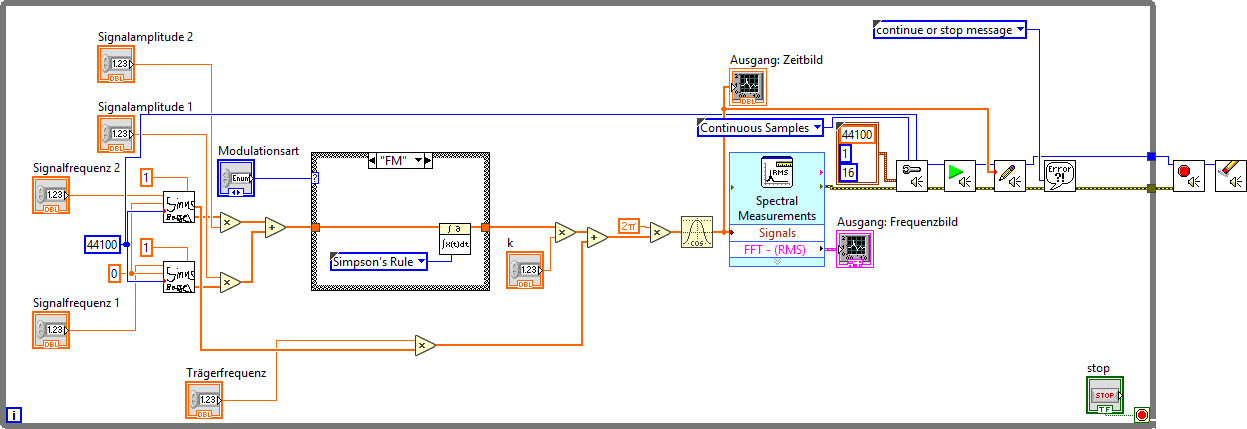
\includegraphics[width=1.0\textwidth]{EIRE2018Dateien/Tag4/FMPM-Erzeugung/FMPM-Erzeugungd}
		\caption{In dieser Abbildung ist das LabVIEW-Blockdiagramm bzw. der Programmcode zu sehen, mit dem ein (Ursprungs-)Signal zuerst wahlweise phasen- oder frequenzmoduliert und anschließend über die Computer-Soundkarte ausgeben wird.}
		\label{FMProgrammcode}
	\end{figure}

	\noindent Die Blockdiagrammobjekte, welche die Ausgabe über die Computer-Soundkarte realisieren, liegen rechtsseitig im Programmcode und teilweise außerhalb der While-Schleife. 
	Deren Anordnung und Funktionsweise ist die gleiche wie beim LabVIEW-Programm in \cref{AMSignalErzeugung}. 
	Genauso wie in \cref{fig_tag3_am_soundkarte_block} aus \cref{AMSignalErzeugung} sieht man auf der linken Seite des Programmcodes zunächst die Erzeugung des (Ursprungs-)Signals $s(t)$ gemäß \cref{Ursprungssignal}. 
	Weiterhin ist dabei die zusätzliche, aufgrund des in \cref{sinusfkt} aufgetretenen Programmierfehlers notwendige Amplitudenmultiplikation zu beachten. 
	Außerdem soll $N = 44.100$ gelten. 
	Da der Vorgang der $s(t)$-Konstruktion komplett identisch zu der in \cref{AMSignalErzeugung} bereits ausführlich beschriebenen Vorgehensweise ist, wird an dieser Stelle nicht weiter auf die (Ursprungs-)Signalentstehung eingegangen. 
	Zwischen den Blockdiagrammobjekten zur Benutzeroberflächenkonfiguration und der (Ursprungs-)Signalentstehung findet im Programmcode die Modulation des Signals statt. 
	Durch das Hinzufügen einer Case-Konstruktion kommt die Auswahlmöglichkeit zwischen Frequenz- und Phasenmodulation zustande. 
	Dazu werden zwei Case-Optionen mit den jeweiligen Markierungen \glqq FM\grqq\ und \glqq PM\grqq\ erstellt. 

	\begin{figure}[H]
		\centering
		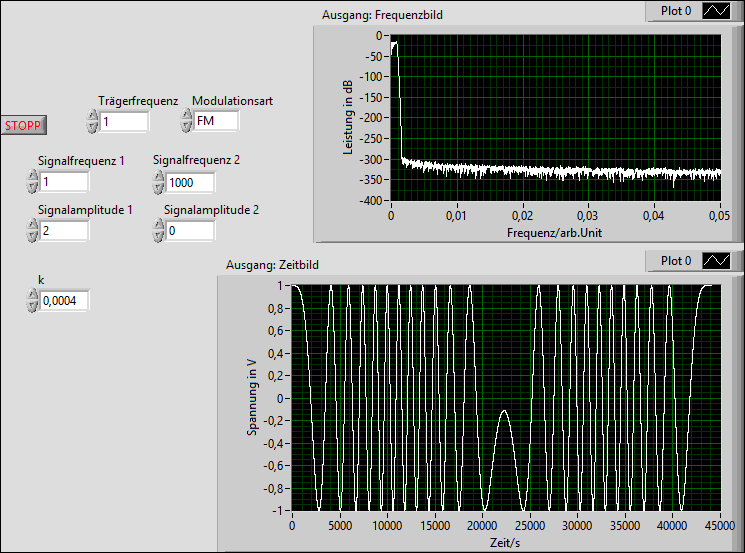
\includegraphics[width=1.0\textwidth]{EIRE2018Dateien/Tag4/FMPM-Erzeugung/FM-FMPM-Erzeugungp}
		\caption{Die Abbildung zeigt das Frontpanel bzw. die Benutzeroberfläche des LabVIEW-Programms zur Umsetzung der Frequenzmodulation. Der hierbei verwendete $k$-Wert ist relativ klein. Allgemein besteht mit dem entsprechenden, sich oben auf dem Frontpanel befindenden Bedienelement die Möglichkeit die Art der Modulation auszuwählen: Entweder Frequenzmodulation (Abkürzung: FM) oder Phasenmodulation (Abkürzung: PM).}
		\label{FMAusgabekleinesk}
	\end{figure}
	
	\noindent Die zwei dadurch erscheinenden, zunächst freien sowie ausfüllbaren Case-Felder sollen somit jeweils der Frequenzmodulation und der Phasenmodulation zur Verfügung stehen. 
	Der Wechsel zwischen diesen beiden erfolgt durch ein mit dem Namen \glqq Modulationsart\grqq\ gekennzeichnetes Bedienelement auf der Benutzeroberfläche samt dazugehörigem Controler an der entsprechenden Stelle im Programmcode.
	
	Im Folgenden wird zwischen Frequenz- und Phasenmodulation (FM und PM) unterschieden. 
	Außerdem wird die Funktionsweise des LabVIEW-Programms näher erläutert.
	
	Die Frequenzmodulation des (Ursprungs-)Signals $s(t)$ soll gemäß der Gleichung
	
	\begin{equation} \label{FMFormel}
	S_{FM}(t) = \cos (2\pi (f_0 t + k \cdot \int s(t) dt))
	\end{equation}
	
	\noindent geschehen, wobei $t$ die Zeit, $f_0$ die sogenannte Trägerfrequenz und $k$ eine beliebige Konstante ist. 
	Am Programmcode in \cref{FMProgrammcode} lässt sich die unter Verwendung der von LabVIEW zur Verfügung gestellten numerischen Operationen, Funktionen und Konstanten erfolgte Umsetzung dieser Formel betrachten. 
	
	\begin{figure}[H]
		\centering
		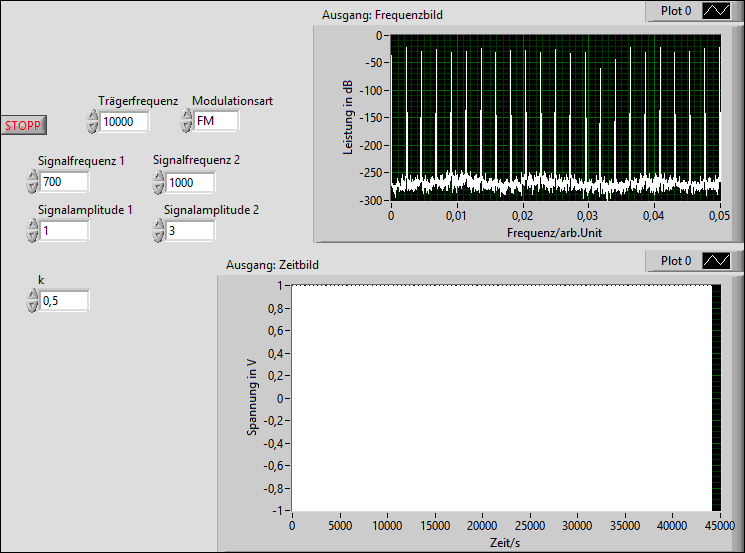
\includegraphics[width=1.0\textwidth]{EIRE2018Dateien/Tag4/FMPM-Erzeugung/anderekbei10000Traegerfr/FM-FMPM-Erzeugungp}
		\caption{In der Abbildung ist das Frontpanel bzw. die Benutzeroberfläche des LabVIEW-Programms zur Realisierung der Frequenzmodulation zu sehen. Der dabei betrachtete $k$-Wert ist vergleichsweise groß.}
		\label{FMAusgabegrossesk}
	\end{figure}
	
	\noindent Unter anderem können die dafür benötigten $t$-Werte, welche nach \cref{t} für alle $i = 0,1,2,...,44.100$ gegeben sind, am Ausgangsanschluss des aus \cref{sinusfkt} stammenden, Sinus-erstellenden Programms abgegriffen werden. 
	Das dazugehörige Blockdiagrammobjekt befindet sich im linken Programmcode-Bereich, welcher der (Ursprungs-)Signalerzeugung dient. 
	Durch zusätzliche Controler und entsprechende Bedienelemente auf dem Frontpanel wird die Eingabe der Gleitkommazahlenwerte für $f_0$ und $k$ realisierbar. 
	Innerhalb des für die Frequenzmodulation reservierten, freien, ausfüllbaren Case-Feldes (\glqq FM\grqq) wird die in \cref{FMFormel} auftretende Integration von $s(t)$ ermöglicht. 
	Dabei wird auf die Simpsonregel (\glqq Simpson's Rule\grqq ) zurückgegriffen, da diese im Vergleich zu anderen bekannten Verfahren der numerischen Integration am effizientesten ist. 
	
	\begin{figure}[H]
		\centering
		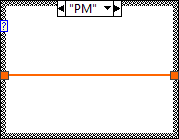
\includegraphics[width=0.8\textwidth]{EIRE2018Dateien/Tag4/FMPM-Erzeugung/PM-FMPM-Erzeugungd1} %Möglicherweise ist 0.8 immer noch zu groß
		\caption{Es ist der in \cref{FMProgrammcode} nicht sichtbare Teil des LabVIEW-Programmcodes dargestellt, der notwendig ist, um die Art der Modulation auf der Benutzeroberfläche des Programms auszuwählen zu können. Bei diesem hier abgebildeten Programmcodeteil handelt es sich um eine weitere Option in der Case-Konstruktion, welche darauf abzielt die Phasenmodulation zu ergänzen.}
		\label{PMProgrammcode}
	\end{figure}
	
	\noindent Die gesamte Berechnung (FM-/PM-Modulation sowie (Ursprungs-)Signalerzeugung) und der Großteil der Signalausgabe finden in einer While-Schleife statt, was auch aus \cref{FMProgrammcode} hervorgeht. 
	Ebenso wie bei den zuvor behandelten Abschnitten ist der While-Schleife ein \glqq Stopp\grqq -Knopf beigefügt, um das Programm bei Bedarf anhalten zu können.

	Vergleicht man die Diagramme des frequenzmodulierten Signals in \cref{FMAusgabekleinesk} mit denen aus \cref{FMAusgabegrossesk}, so lässt sich feststellen, dass im Zeitbild die tausendfach höhere Trägerfrequenz deutlich zum Tragen kommt, sodass zahlreiche Nulldurchgänge stattfinden. 
	Der Graph erscheint daher wie ein \glqq weißer Block\grqq\ aus Linien. 
	Der Vergleich der beiden Frequenzbilder legt die Vermutung nahe, dass die Vergrößerung des $k$-Wertes zu schärfer definierten Peaks im Frequenzspektrum führt.
	
	Phasenmoduliert man das Ursprungssignal $s(t)$, so nimmt das daraus entstehende Signal $S_{PM}(t)$ die Form
	
	\begin{equation} \label{PMFormel}
	S_{PM}(t) = \cos (2\pi (f_0 t + k \cdot s(t)))
	\end{equation}
	
	\noindent an. 
	Dabei bildet $f_0$ die Trägerfrequenz und $t$ die Zeit. 
	$k$ ist ein fester, aber beliebig wählbarer Faktor. 
	Aufgrund der Ähnlichkeit von \cref{PMFormel} zu \cref{FMFormel}, verläuft auch die Realisierung der Phasenmodulation als LabVIEW-Programm ähnlich zur Programm-Umsetzung der Frequenzmodulation. 
	
	\begin{figure}[H]
		\centering
		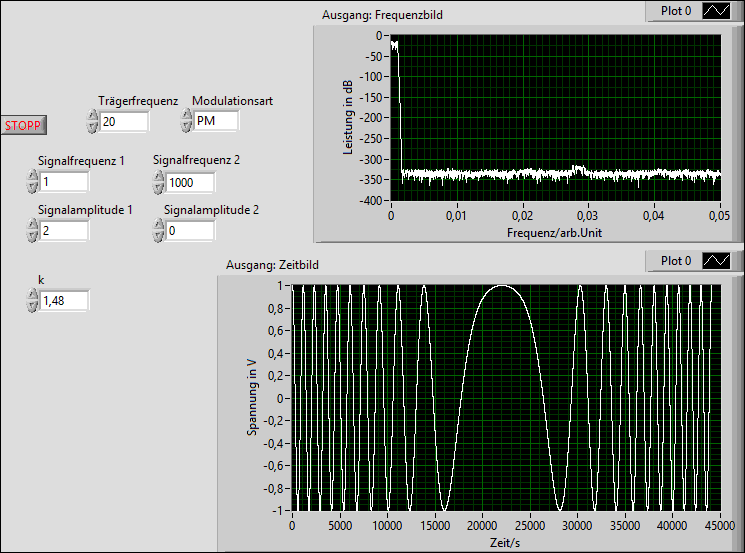
\includegraphics[width=1.0\textwidth]{EIRE2018Dateien/Tag4/FMPM-Erzeugung/PM-FMPM-Erzeugungp}
		\caption{Die Abbildung zeigt das Frontpanel bzw. die Benutzeroberfläche des LabVIEW-Programms zur Realisierung der Phasenmodulation.}
		\label{PMAusgabe}
	\end{figure}

	\noindent Daher besteht lediglich die Notwendigkeit das für die Phasenmodulation reservierte, freie, ausfüllbare Case-Feld passend zu besetzen. 
	Wie im Programmcode in \cref{PMProgrammcode} zu erkennen, wird hierbei die Leitung direkt durch das Case-Feld gezogen, ohne das übertragene Signal zu bearbeiten oder zu verändern. 
	In Kombination mit der bereits durch die Frequenzmodulation existierenden Programm-Struktur ist damit die Umsetzung der Phasenmodulation abgeschlossen. 
	Das sich ergebene, phasenmodulierte Signal $S_{PM}(t)$ bzw. $\tilde{S}_{PM}(f)$ ist in den beiden Diagrammen auf der Benutzeroberfläche des Programms aus \cref{PMAusgabe} dargestellt.
	
	\emph{Hinweis:} Bei diesem LabVIEW-Programm zur Erzeugung von phasen- und frequenzmodulierten Signalen ist zu beachten, dass zwischen den $k$-Werten der Frequenzmodulation und den $k$-Werten der Phasenmodulation stets eine Diskrepanz um einen Faktor der Größenordnung $10^4$ vorliegt.
	
	
	
	\subsection{Demodulation eines phasen- bzw. frequenzmodulierten Signals}
	
	Im Folgenden soll ein über den Analog-Digital-Wandler in Kombination mit der Computer-Soundkarte gemessenes Signal, welches entweder phasen- oder frequenzmoduliert wurde, demoduliert werden. 
	Das in \cref{DemodTraeger} erhaltene LabVIEW-Programm dient dabei als Vorlage. 
	Von links nach rechts gelesen, beinhaltet dessen Programmcode, welcher in \cref{MultiTraegerProgrammcode} dargestellt ist, einen Programmteil zur Messdatenaufnahme mittels Analog-Digital-Wandler, einen für die Demodulation von AM-Signalen zuständigen Programmbereich, einen Tiefpassfilter sechzehnter Ordnung, einige Blockdiagrammobjekte zur Realisierung der Anzeige- bzw. Ausgabeelemente auf dem Frontpanel, eine durch den sich auf der Benutzeroberfläche befindlichen \glqq Stopp\grqq -Knopf und eine Speicherfunktion mit dazugehörigem \glqq Speichern\grqq -Knopf.
	
	
	Der Tiefpass wird auf einen Bandpass erweitert, wobei die obere und untere Grenzfrequenz 
	
	\begin{figure}[H]
		\centering
		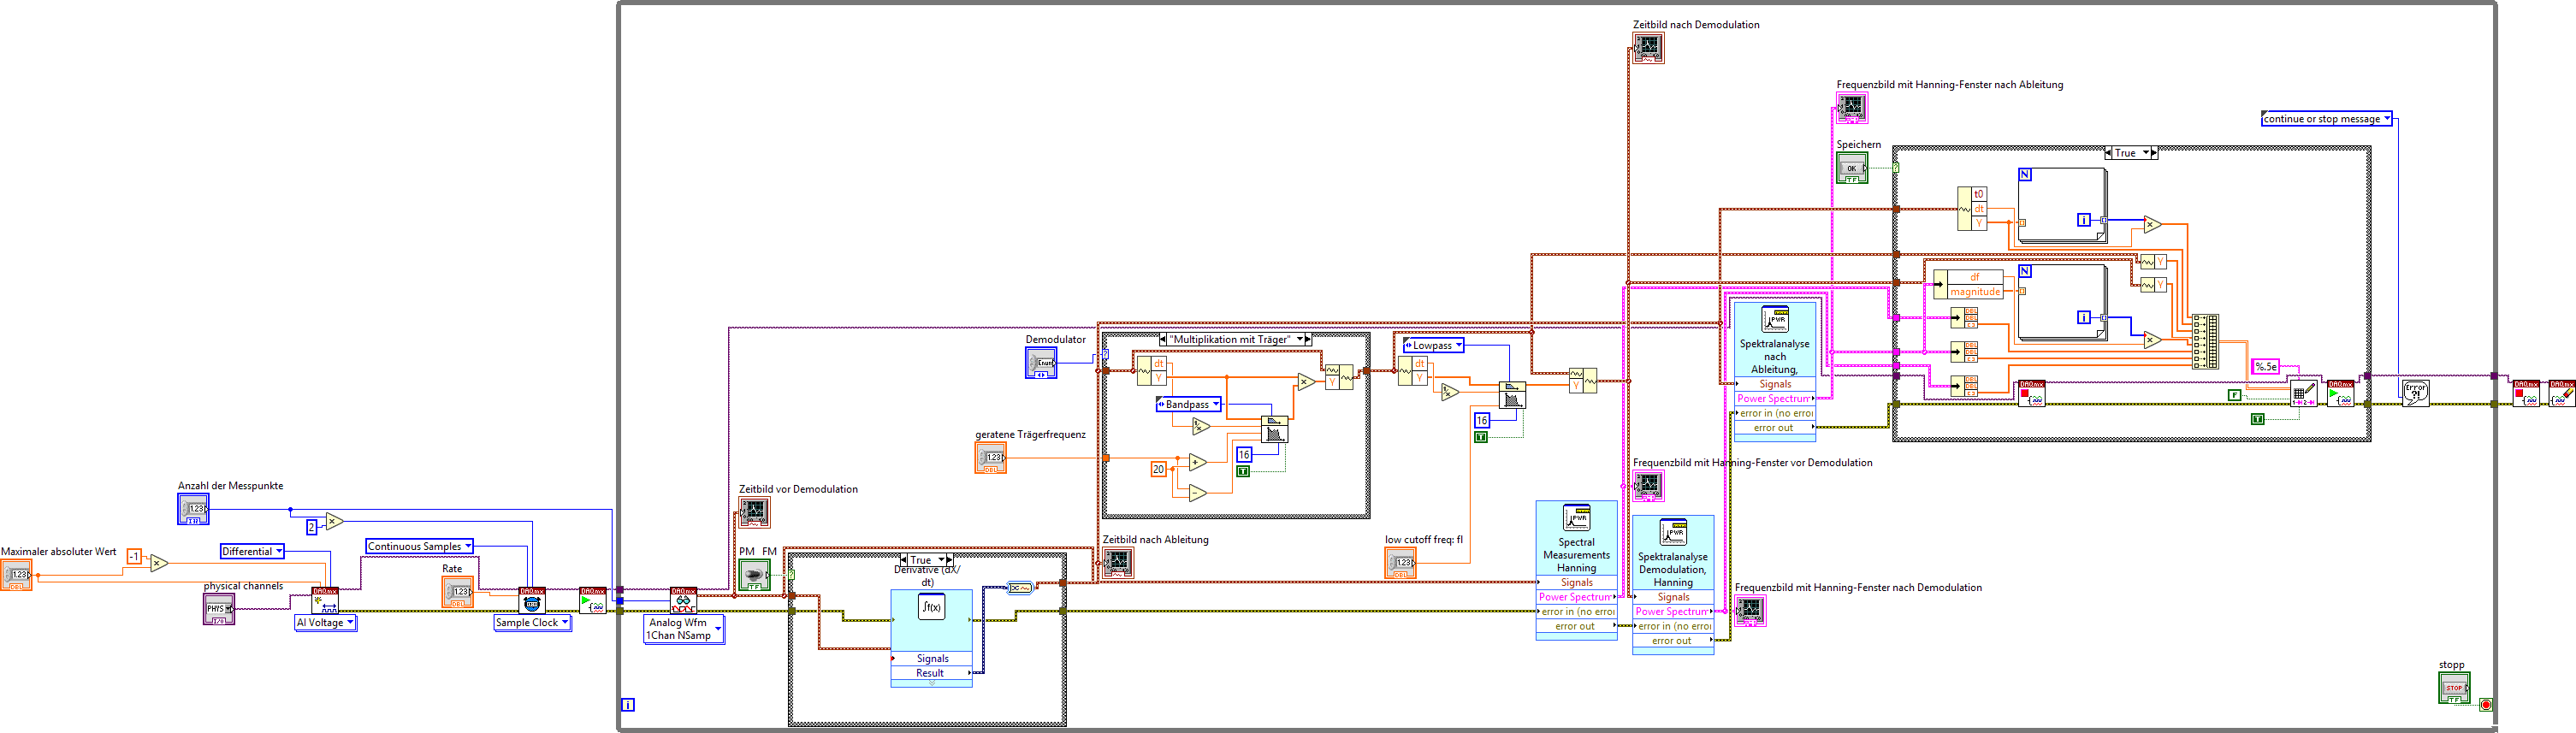
\includegraphics[width=1.0\textwidth]{EIRE2018Dateien/Tag4/OsziFMPM-Demod/FM/OsziPlusFMPMd}
		\caption{.}
	\end{figure}
	
	\begin{figure}[H]
		\centering
		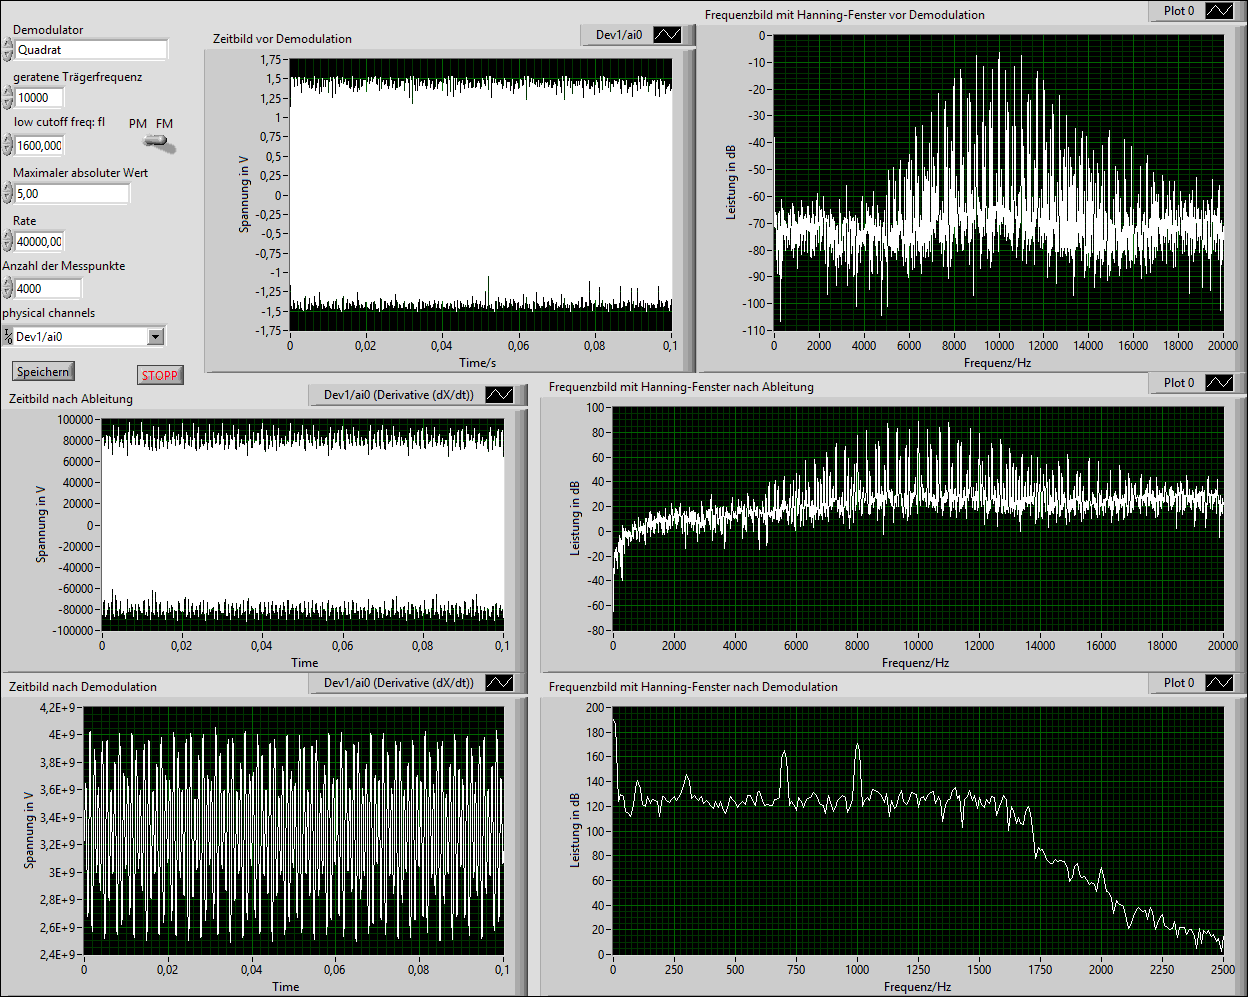
\includegraphics[width=1.0\textwidth]{EIRE2018Dateien/Tag4/OsziFMPM-Demod/FM/OsziPlusFMPMp}
		\caption{.}
	\end{figure}
	
	\begin{figure}[H] %FM-Diagramm
		\centering
		\includegraphics[width=1.0\textwidth]{EIRE2018Dateien/Tag4/OsziFMPM-Demod/FM/Frequenzbild_mit_Hanning_nach_TP_und_Demod_k0,005}
		\caption{.}
	\end{figure}
	
	\begin{figure}[H]
		\centering
		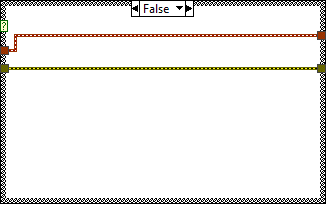
\includegraphics[width=0.8\textwidth]{EIRE2018Dateien/Tag4/OsziFMPM-Demod/PM/OsziPlusFMPMd5} %Möglicherweise ist 0.8 immer noch zu groß
		\caption{.}
	\end{figure}
		
	\begin{figure}[H] %PM-Diagramm
		\centering
		\includegraphics[width=1.0\textwidth]{EIRE2018Dateien/Tag4/OsziFMPM-Demod/PM/Frequenzbild_mit_Hanning_nach_TP_und_Demod_k0,1}
		\caption{.}
	\end{figure}
	
	
	
	%Fktion nur schön für bestimmten Bereich von k, weil , wenn zu hoch: zu viele Oberwellen, zu klein: demoduliertes Signal geht im Rauschen unter
	\subsection{Erweiterte Demodulation mit Bandpass und zusätzlicher Integration des Signals}
	
	
	
	\begin{figure}[H]
		\centering
		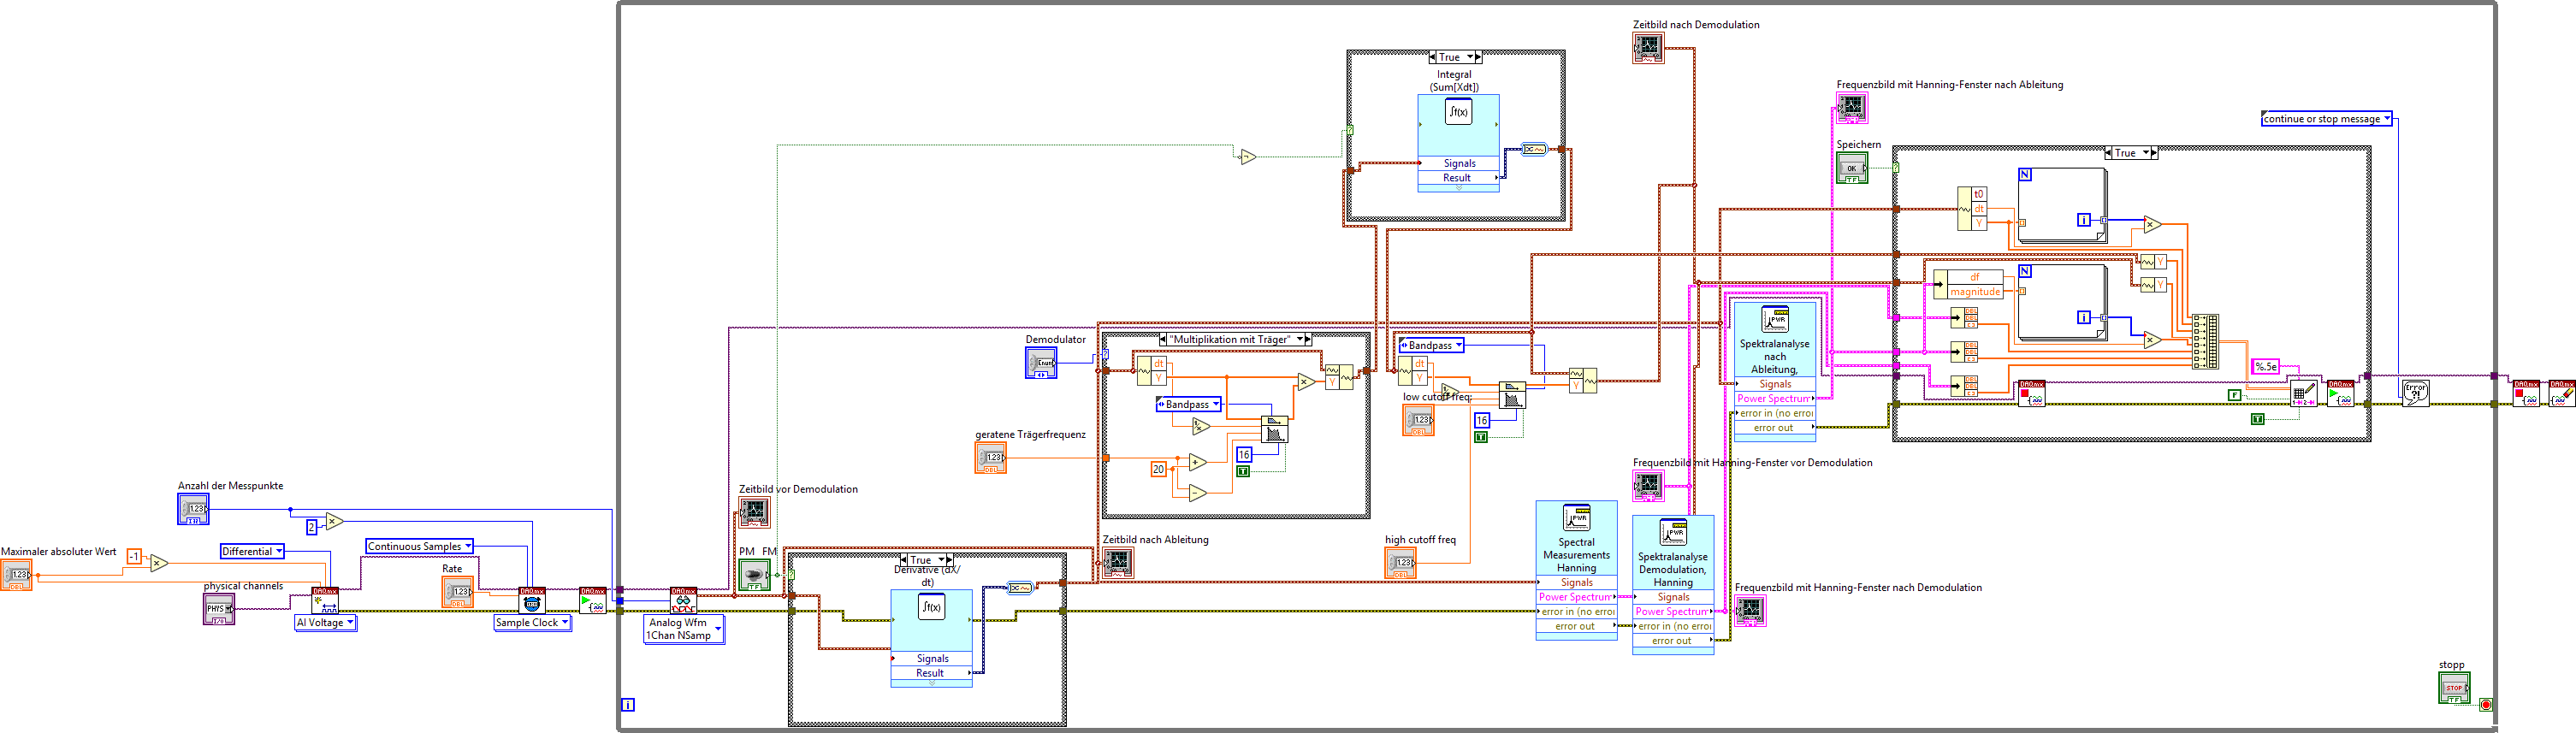
\includegraphics[width=1.0\textwidth]{EIRE2018Dateien/Tag4/OsziFMPM-Demod/mitBandpassUndIntegrationBilder/OsziPlusFMPMd}
		\caption{.}
	\end{figure}
	
	\begin{figure}[H]
		\centering
		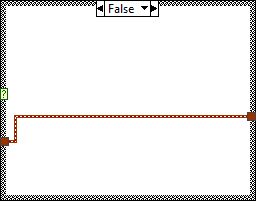
\includegraphics[width=0.8\textwidth]{EIRE2018Dateien/Tag4/OsziFMPM-Demod/mitBandpassUndIntegrationBilder/OsziPlusFMPMd6} %Möglicherweise ist 0.8 immer noch zu groß
		\caption{.}
	\end{figure}
		
	\begin{figure}[H]
		\centering
		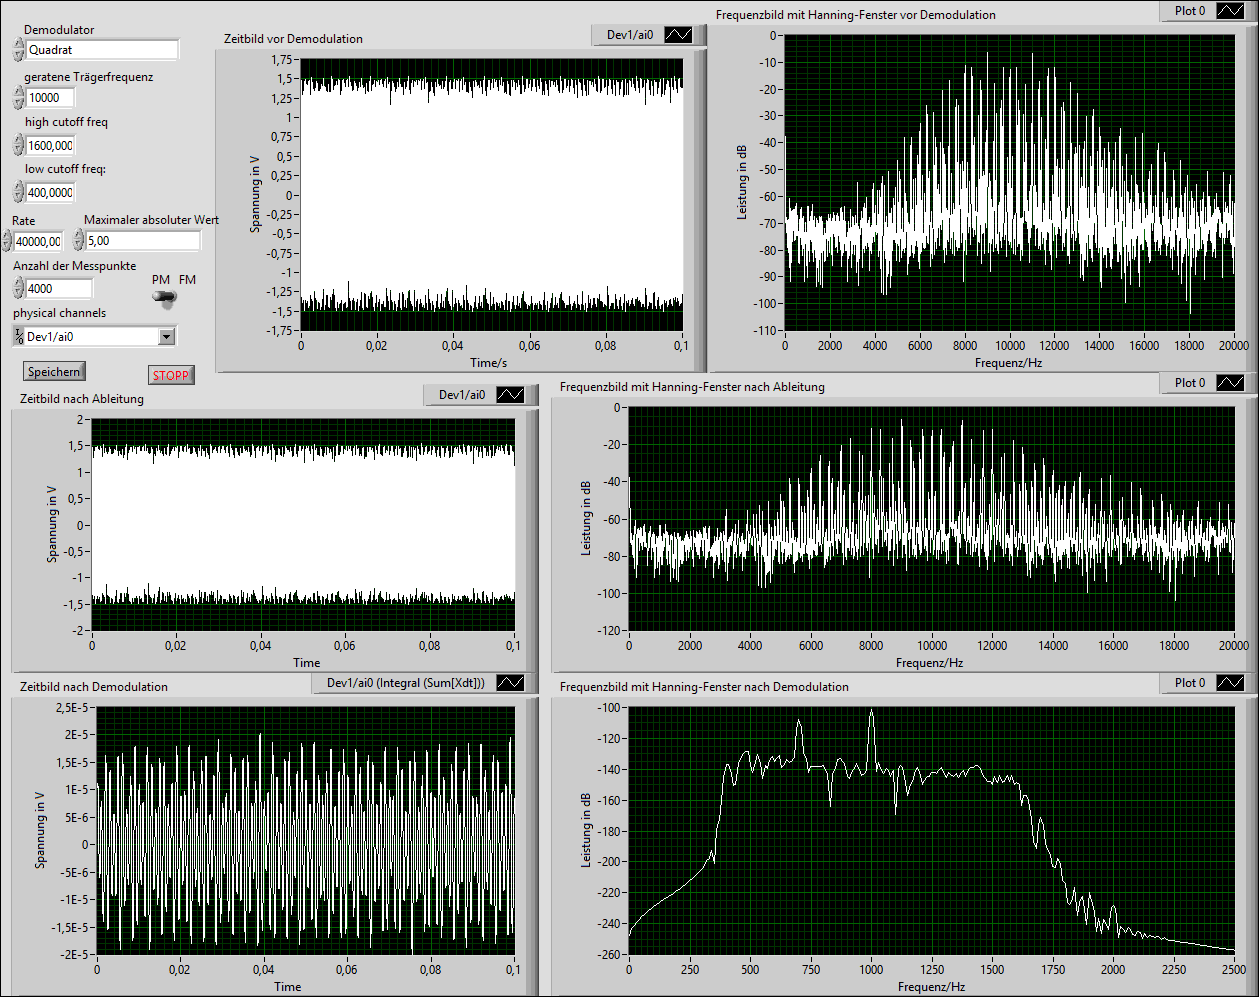
\includegraphics[width=1.0\textwidth]{EIRE2018Dateien/Tag4/OsziFMPM-Demod/mitBandpassUndIntegrationBilder/OsziPlusFMPMp}
		\caption{.}
	\end{figure}
	
	\begin{figure}[H] %FM-Diagramm mit Bandpass
		\centering
		\includegraphics[width=1.0\textwidth]{EIRE2018Dateien/Tag4/OsziFMPM-Demod/FMmitBandpassundInt/Frequenzbild_mit_Hanning_nach_BP_und_Demod}
		\caption{.}
	\end{figure}
	
	\begin{figure}[H] %PM-Diagramm mit Bandpass und Integration 
		\centering
		\includegraphics[width=1.0\textwidth]{EIRE2018Dateien/Tag4/OsziFMPM-Demod/PMmitBandpassundInt/Frequenzbild_mit_Hanning_nach_BP,Int,Demod}
		\caption{.}
	\end{figure}
	
	
	\printbibliography %ist bissl un
	
	
\end{document}
